\documentclass[extrafontsizes,14pt]{memoir}
% Base fonts available for memoir are:
% 9pt, 10pt, 11pt, 12pt, 14pt, 17pt, 20pt, 25pt,
% 30pt, 36pt, 48pt and 60pt
% When using fonts larger than 12, you also
% have to
%, e.g. \documentclass[extrafontsizes,20pt]{memoir}
%
% The best font size for a printed service book used by the clergy is 14.
% For a printed service book used by the people, set it to 11 or 12.
% For a PDF to be viewed on a smart phone or a tablet, set it to 20.
%
%
% Note: keys must not have an underscore _ as part of the value.
%
%
\usepackage[hyphenate]{system/ocmc-liturgical-text} % includes packages and creates new commands
% Author: Michael Colburn
% Purpose: controls various options for typesetting liturgical text

%==================================================
% {ara}{ara} = in Arabic what is the name of ara?
% {ara}{en} = in Arabic what is the name of en?
\itId{sys}{iso}{language.code}{ara}{ara}{%
العربية
}%
\itId{sys}{iso}{language.code}{ara}{en}{%
الإنجليزية
}%
\itId{sys}{iso}{language.code}{ara}{gr}{%
اللغة اليونانية
}%
\itId{sys}{iso}{language.code}{ara}{heb}{%
اللغة العبرية
}%
\itId{sys}{iso}{language.code}{ara}{swh}{%
السواحلية
}%
\itId{sys}{iso}{language.code}{ara}{yid}{%
اليديشية
}%
% in English, what is the name of code?
\itId{sys}{iso}{language.code}{en}{ara}{%
Arabic
}%
\itId{sys}{iso}{language.code}{en}{chu}{%
Church Slavonic
}%
\itId{sys}{iso}{language.code}{en}{en}{%
English
}%
\itId{sys}{iso}{language.code}{en}{fra}{%
French
}%
\itId{sys}{iso}{language.code}{en}{gr}{%
Greek
}%
\itId{sys}{iso}{language.code}{en}{heb}{%
Hebrew
}%
\itId{sys}{iso}{language.code}{en}{kik}{%
Kikuku
}%
\itId{sys}{iso}{language.code}{en}{swh}{%
Swahili
}%
\itId{sys}{iso}{language.code}{en}{ukr}{%
Ukrainian
}%
\itId{sys}{iso}{language.code}{en}{yid}{%
Yiddish
}%
% Greek
\itId{sys}{iso}{language.code}{gr}{gr}{%
Ελληνικά
}%
\itId{sys}{iso}{language.code}{gr}{en}{%
Αγγλικά
}%
\itId{sys}{iso}{language.code}{gr}{swh}{%
Σουαχίλι
}%
\itId{sys}{iso}{language.code}{gr}{ara}{%
Arabic
}%
\itId{sys}{iso}{language.code}{gr}{heb}{%
Εβραϊκά
}%
\itId{sys}{iso}{language.code}{gr}{yid}{%
Γερμανοεβραϊκή Διάλεκτος
}%
% Hebrew
\itId{sys}{iso}{language.code}{heb}{ara}{%
עֲרָבִית
}%
\itId{sys}{iso}{language.code}{heb}{en}{%
אנגלית
}%
\itId{sys}{iso}{language.code}{heb}{gr}{%
יווני
}%
\itId{sys}{iso}{language.code}{heb}{heb}{%
עִברִית
}%
\itId{sys}{iso}{language.code}{heb}{swh}{%
סוואהילית
}%
\itId{sys}{iso}{language.code}{heb}{yid}{%
אִידִישׁ
}%
% Swahili
\itId{sys}{iso}{language.code}{swh}{en}{%
English
}%
\itId{sys}{iso}{language.code}{swh}{gr}{%
Greek
}%
\itId{sys}{iso}{language.code}{swh}{swh}{%
Swahili
}%
\def\ltClientPath{your.choices/ke.oak}
%=================================================
% CLIENT SETTINGS FILE
%=================================================
\def\clientCountry{ke} % get code from https://en.wikipedia.org/wiki/ISO_3166-1_alpha-3
\def\clientAcronymn{oak} % ask client what to use
\setbool{blessed}{false} % set true when get blessing
%==================================================
% Which language or languages?
%
% Controls language or languages to use.
% Each language must have a folder with that name
% in the resources folder, e.g. resources/gr_gr_cog
%
%\ltSetPrimaryDomain{gr}{gr}{cog}
%\ltSetCenterDomain{swh}{ke}{oak}
%\ltSetRightDomain{en}{uk}{lash}

%\ltSetPrimaryDomain{en}{uk}{lash}
%\ltSetCenterDomain{swh}{ke}{oak}
%\ltSetRightDomain{kik}{ke}{oak}

%\ltSetPrimaryDomain{en}{uk}{lash}
%\ltSetCenterDomain{swh}{ke}{oak}
%\ltSetRightDomain{gr}{gr}{cog}

\ltSetPrimaryDomain{en}{uk}{lash}
%\ltSetRightDomain{swh}{ke}{oak}

%ltSetPrimaryDomain{en}{uk}{lash}
%\ltSetRightDomain{gr}{gr}{cog}

% This will load the specified resource file
%for each domain we declared above.
\ltLoadResources{liturgystjohn}
%\ltLoadResources{baptism}
%\ltLoadResources{eu.baptism}
%\ltLoadResources{blessingbuildingorbusiness}
%\ltLoadResources{childbirth}
%\ltLoadResources{churchdedicationatvespers}
%\ltLoadResources{holyunction}
\ltLoadResources{matinsforsunday}
%\ltLoadResources{matinsweekday}
%\ltLoadResources{trisagion}
%\ltLoadResources{typika}
%\ltLoadResources{vespersforsunday}
%\ltLoadResources{wedding}

%\ltLoadResources{a.has.problems}
%\ltLoadResources{actors}
%\ltLoadResources{client}
%\ltLoadResources{copyright}
%\ltLoadResources{dismissals}
%\ltLoadResources{duplicates}
%\ltLoadResources{eu.lichrysbasil}
%\ltLoadResources{ho.s03}
%\ltLoadResources{ho.s21}
%\ltLoadResources{me.m10.d28}
%\ltLoadResources{misc}
%\ltLoadResources{pe.d00P}
%\ltLoadResources{prayers}
%\ltLoadResources{ps.kenya.alt}
%\ltLoadResources{ps}
%\ltLoadResources{pub.priest.servicebook}
%\ltLoadResources{rubrical}
%\ltLoadResources{titles}
%=================================================
% COVER PAGE
% Add a key for each domain you use
%=================================================
\itId{gr}{gr}{cog}{client.settings}{client.title}{%
ΤΟ ΠΑΤΡΙΑΡΧΕΙΟ ΑΛΕΞΑΝΔΡΕΙΑΣ ΚΑΙ ΠΑΣΗΣ ΑΦΡΙΚΗΣ
}
\itId{en}{uk}{lash}{client.settings}{client.title}{%
GREEK ORTHODOX PATRIARCHATE OF \\ALEXANDRIA AND ALL AFRICA
}
\itId{gr}{gr}{cog}{client.settings}{cover.title}{%
ΙΕΡΑΤΙΚΟΝ
}
\itId{heb}{isr}{aaawf}{client.settings}{cover.title}{%
ΙΕΡΑΤΙΚΟΝ
}
\itId{ara}{isr}{aaawf}{client.settings}{cover.title}{%
ΙΕΡΑΤΙΚΟΝ
}
\itId{en}{uk}{lash}{client.settings}{cover.title}{%
Priest's Service Book
}
\itId{shw}{ke}{oak}{client.settings}{cover.title}{%
Priest's Service Book
}
%=================================================
% COPYRIGHT PAGE
%=================================================
\itId{sys}{client.settings}{\clientCountry}{\clientAcronymn}{copyright}{%
\itRid{client.settings}{client.title}\ except as noted above.
}%
\itId{sys}{client.settings}{\clientCountry}{\clientAcronymn}{publisher}{%
TBD
}%
\itId{sys}{client.settings}{\clientCountry}{\clientAcronymn}{patriarch}{%
HIS ALL-HOLINESS THEOPHILOS III PATRIARCH OF JERUSALEM
}%
\itId{sys}{client.settings}{\clientCountry}{\clientAcronymn}{bishop}{%
}%
\itId{sys}{client.settings}{\clientCountry}{\clientAcronymn}{for.use.in}{%
the Dioceses of Israel
}%

%==================================================
% Actors on separate line?
%
% Controls whether the actor will appear on its on line.
% For example, 
%
% If enabled:
% Priest: In the name of the Father and of the Son...
%
% If not enabled:
% Priest
% In the name of the Father and of the Son...
%
%\def\actorOnSeparateLine{} % comment out to display actor on separate line
% 
%==================================================


%==================================================
%=========================================================
% Global Settings
%=========================================================
% set page margin:
\geometry{margin=1in} % see package geometry for options
% set paragraph indent.  
\setlength{\parindent}{0em}
\setlength{\JustifyingParindent}{0em}
% set spacing between paragraphs.  0.5em is usual
\setlength{\parskip}{1em}
\setlength{\JustifyingParfillskip}{1em}

% memoir package settings
\setsecnumdepth{none}
\maxsecnumdepth{none}
\titleformat{\section}[block]{\color{blue}\Large\bfseries\filcenter}{}{0.5em}{}
\pagestyle{ruled}

% header and footer settings
% \leftmark is the chapter title
% \rightmark is the section title.
\makeevenhead{ruled}{}{\rightmark}{\thepage}
\makeoddhead{ruled}{\thepage}{\leftmark}{}
\makeevenfoot{ruled}{}{}{}
\makeoddfoot{ruled}{}{}{}
\setbool{subsectionInHeader}{true}% false to turn off 
{\addtolength{\beforechapskip}{1\baselineskip}}
{\addtolength{\afterchapskip}{1\baselineskip}}

% to help with avoiding overfull 
% hbox with narrow columns.
% Note that the max is 10000 for h or vbadness.
% If you set to 10000 completely ignores.
% 9999 is tolerant of anything up to 10000
\def\mysloppy{%
  \tolerance=9999
  \setlength{\emergencystretch}{0.5em}
  \hfuzz 1pt
  \vfuzz=\hfuzz
  \hbadness=9999
  \vbadness=\maxdimen
}
 % control.tex allows you to easily change settings

\ltDebugOn%

\begin{document}

\ltCover

\frontmatter

\ltCopyRight{}

\pagebreak

\tableofcontents

\vfill

\pagebreak

\ltBlessing

\ltPreface

\mainmatter

\ltColumnsOn
%\begin{multicols}{2}

%\ltChapter{vespersforsunday}{p0001.title}

\ltSection{vespersforsunday}{p0001b.title}

\ltRubric{vespersforsunday}{p0002}

%Problem: In p0003, the word "Epitrachelion" is underlined

\ltRubric{vespersforsunday}{p0003}

\ltDialog{duplicates}{d0199}

%Problem:In p0005, the word "Gerontika" is underlined 

\ltRubric{vespersforsunday}{p0005}

\ltDialog{prayers}{res04}

\ltDialog{duplicates}{d0243}

\ltDialog{duplicates}{d0240}

\ltDialog{vespersforsunday}{p0009}

\ltRubric{vespersforsunday}{p0010}

\ltDialog{vespersforsunday}{p0011}

%In p0012, the word "Anixantaria" is underlined 

\ltRubric{vespersforsunday}{p0012}

\ltDialog{vespersforsunday}{p0013}

%Problem: when you open your hand is bold

\ltRubric{vespersforsunday}{p0014}

\ltDialog{vespersforsunday}{p0015}

\ltDialog{duplicates}{d0385}

\ltDialog{duplicates}{d0206}


%Problem: In p0019, the words " Sticharion and Orarion" are underlined 

\ltRubric{vespersforsunday}{p0019}

\ltRubric{duplicates}{d0019}

\ltDialog{vespersforsunday}{p0021}

\ltDialog{duplicates}{d0332}

\ltRubric{duplicates}{d0025}

\ltDialog{vespersforsunday}{p0024}

\ltDialog{vespersforsunday}{p0025}

\ltRubric{duplicates}{d0029}

\ltDialog{vespersforsunday}{p0027}

\ltDialog{duplicates}{d0349}

\ltRubric{duplicates}{d0032}

\ltDialog{vespersforsunday}{p0030}

\ltDialog{duplicates}{d0332}

\ltRubric{duplicates}{d0034}

\ltDialog{vespersforsunday}{p0033}

\ltDialog{vespersforsunday}{p0034}

\ltRubric{duplicates}{d0036}

\ltDialog{vespersforsunday}{p0036}

\ltDialog{vespersforsunday}{p0037}

\ltRubric{duplicates}{d0038}

\ltDialog{vespersforsunday}{p0039}

\ltDialog{duplicates}{d0349}

\ltRubric{vespersforsunday}{p0041}

\ltRubric{duplicates}{d0559}

\ltActorDialog{duplicates}{d0251}{duplicates}{d0504}

\ltActorDialogRubric{duplicates}{d0773}{duplicates}{d0585}{duplicates}{d1216}

\ltActorDialog{duplicates}{d0251}{duplicates}{d0318}

\ltDialog{duplicates}{d0319}

\ltDialog{duplicates}{d0326}

\ltDialog{duplicates}{d0291}


%p0053 varies for each country


\ltDialog{duplicates}{d0325}

\ltDialog{duplicates}{d0293}

\ltDialog{duplicates}{d0327}

\ltDialog{duplicates}{d0304}

\ltDialog{duplicates}{d0463}

\ltDialog{duplicates}{d0246}

\ltActorDialog{duplicates}{d0773}{duplicates}{d1054}

\ltActorDialog{duplicates}{d0779}{duplicates}{d0331}

\ltActorDialog{duplicates}{d0773}{prayers}{res04}

\ltRubric{vespersforsunday}{p0066}

%Problem: p0067-p0081 say which hymns to sing, but the original actually shows the psalms

\ltRubric{vespersforsunday}{p0067}

\ltDialog{vespersforsunday}{p0068}

\ltDialog{vespersforsunday}{p0069}

\ltDialog{vespersforsunday}{p0070}

\ltDialog{vespersforsunday}{p0071}

\ltDialog{vespersforsunday}{p0072}

\ltDialog{vespersforsunday}{p0073}

\ltDialog{vespersforsunday}{p0074}

\ltDialog{vespersforsunday}{p0075}

\ltDialog{vespersforsunday}{p0076}

\ltDialog{vespersforsunday}{p0077}

\ltDialog{vespersforsunday}{p0078}

\ltDialog{vespersforsunday}{p0079}

\ltDialog{vespersforsunday}{p0080}

\ltDialog{vespersforsunday}{p0081}

\ltRubric{vespersforsunday}{p0082}

\ltActorDialog{duplicates}{d0251}{duplicates}{d0058}

\ltActorDialog{duplicates}{d0773}{duplicates}{d0575}

\ltActorDialog{duplicates}{d0251}{duplicates}{d0463}

\ltActorDialog{duplicates}{d0773}{duplicates}{d0575}

\ltActorDialog{duplicates}{d0251}{duplicates}{d0246}

\ltActorDialog{duplicates}{d0773}{duplicates}{d1054}

\ltActorDialog{duplicates}{d0779}{vespersforsunday}{p0096}

\ltActorDialog{duplicates}{d0773}{prayers}{res04}

\ltRubricDialogRubric{vespersforsunday}{p0099a}{vespersforsunday}{p0099b}{vespersforsunday}{p0099c}

\ltDialog{duplicates}{d0199}

\ltRubric{vespersforsunday}{p0101}

\ltRubric{vespersforsunday}{p0102}

%Problem: lord I have cried in bold

\ltRubricDialog{duplicates}{d[A]}{vespersforsunday}{p0103}

%Problem: Let my prayer be directed in bold

\ltRubricDialog{duplicates}{d[B]}{vespersforsunday}{p0104}

\ltRubricDialog{duplicates}{d[A]}{vespersforsunday}{p0105}

\ltRubricDialog{duplicates}{d[B]}{vespersforsunday}{p0106}

\ltRubricDialog{duplicates}{d[A]}{vespersforsunday}{p0107}

\ltRubricDialog{duplicates}{d[B]}{vespersforsunday}{p0108}

\ltRubricDialog{duplicates}{d[A]}{vespersforsunday}{p0109}

\ltRubricDialog{duplicates}{d[B]}{vespersforsunday}{p0110}

\ltRubricDialog{duplicates}{d[A]}{vespersforsunday}{p0111}

\ltRubricDialog{duplicates}{d[B]}{vespersforsunday}{p0112}

\ltRubricDialog{duplicates}{d[A]}{vespersforsunday}{p0113}

\ltRubric{vespersforsunday}{p0114}

%Problem with my voice in bold

\ltRubricDialog{duplicates}{d[B]}{vespersforsunday}{p0115}

\ltRubricDialog{duplicates}{d[A]}{vespersforsunday}{p0116}

\ltRubricDialog{duplicates}{d[B]}{vespersforsunday}{p0117}

\ltRubricDialog{duplicates}{d[A]}{vespersforsunday}{p0118}

\ltRubricDialog{duplicates}{d[B]}{vespersforsunday}{p0119}

\ltRubricDialog{duplicates}{d[A]}{vespersforsunday}{p0120}

\ltRubricDialog{duplicates}{d[B]}{vespersforsunday}{p0121}

\ltRubricDialog{duplicates}{d[A]}{vespersforsunday}{p0122}

\ltRubricDialog{duplicates}{d[B]}{vespersforsunday}{p0123}


\ltRubricDialog{vespersforsunday}{p0125a}{vespersforsunday}{p0125b}

\ltRubricDialog{vespersforsunday}{p0126a}{vespersforsunday}{p0126b}


%Problem: out of the depths in bold

\ltRubric{vespersforsunday}{p0128}

\ltRubricDialog{vespersforsunday}{p0129a}{vespersforsunday}{p0129b}

\ltRubricDialog{vespersforsunday}{p0130a}{vespersforsunday}{p0130b}

\ltRubric{vespersforsunday}{p0131}

\ltRubricDialog{vespersforsunday}{p0132a}{vespersforsunday}{p0132b}

\ltRubricDialog{vespersforsunday}{p0133a}{vespersforsunday}{p0133b}

\ltRubric{duplicates}{d0286}

\ltRubricDialog{vespersforsunday}{p0135a}{vespersforsunday}{p0135b}

\ltRubricDialog{vespersforsunday}{p0136a}{vespersforsunday}{p0136b}

%Problem: praise the lord in bold

\ltRubric{vespersforsunday}{p0137}

\ltRubricDialog{vespersforsunday}{p0138a}{vespersforsunday}{p0138b}

\ltRubricDialog{vespersforsunday}{p0139a}{vespersforsunday}{p0139b}

\ltDialog{vespersforsunday}{p0140}

\ltRubric{vespersforsunday}{p0141}

\ltDialog{duplicates}{d0551}

\ltRubric{vespersforsunday}{p0143}

\ltRubric{vespersforsunday}{p0144}

\ltDialog{vespersforsunday}{p0145}

\ltDialog{duplicates}{d0332}

\ltRubric{vespersforsunday}{p0147}

\ltDialog{vespersforsunday}{p0148}

\ltRubric{vespersforsunday}{p0149}

\ltDialog{vespersforsunday}{p0150}

\ltActorDialog{duplicates}{d0251}{prayers}{res04}

\ltRubric{vespersforsunday}{p0153}

\ltDialog{duplicates}{d1145}

\ltRubric{vespersforsunday}{p0155}

\ltRubric{vespersforsunday}{p0156}

\ltRubric{vespersforsunday}{p0157}

\ltRubric{vespersforsunday}{p0158}

\ltDialog{vespersforsunday}{p0159}

\ltRubric{vespersforsunday}{p0160}

%Problem prokemenon underlined

\ltActorDialog{vespersforsunday}{p0161a}{vespersforsunday}{p0161b}

\ltRubric{duplicates}{d0697}

\ltRubric{duplicates}{d1085}

\ltDialog{duplicates}{d0903}

\ltRubricDialog{vespersforsunday}{p0165a}{vespersforsunday}{p0165b}

\ltDialog{duplicates}{d0903}

\ltRubricDialog{vespersforsunday}{p0167a}{vespersforsunday}{p0167b}

\ltDialog{vespersforsunday}{p0168}

\ltRubric{vespersforsunday}{p0169}

\ltRubric{duplicates}{d1090}


\ltRubricDialog{vespersforsunday}{p0172a}{vespersforsunday}{p0172b}

\ltDialog{vespersforsunday}{p0173}

\ltRubric{vespersforsunday}{p0174}

\ltRubric{duplicates}{d1080}

\ltDialog{vespersforsunday}{p0176}

\ltRubricDialog{vespersforsunday}{p0177a}{vespersforsunday}{p0177b}

\ltRubric{vespersforsunday}{p0178}

\ltRubric{duplicates}{d1068}

\ltDialog{vespersforsunday}{p0180}

\ltRubricDialog{vespersforsunday}{p0181a}{vespersforsunday}{p0181b}

\ltRubric{vespersforsunday}{p0182}

\ltRubric{duplicates}{d1084}

\ltDialog{vespersforsunday}{p0184}

\ltRubricDialog{vespersforsunday}{p0185a}{vespersforsunday}{p0185b}

\ltRubric{vespersforsunday}{p0186}

\ltRubric{duplicates}{d1085}

\ltDialog{vespersforsunday}{p0188}

\ltRubricDialog{vespersforsunday}{p0189a}{vespersforsunday}{p0189b}

\ltRubric{vespersforsunday}{p0190}

\ltRubric{duplicates}{d1088}

\ltDialog{vespersforsunday}{p0192}

\ltRubricDialog{vespersforsunday}{p0193a}{vespersforsunday}{p0193b}

\ltRubric{vespersforsunday}{p0194}

\ltRubric{duplicates}{d0558}

\ltActorDialog{duplicates}{d0251}{duplicates}{d0535}

\ltActorDialog{duplicates}{d0773}{duplicates}{d0575}

\ltActorDialog{duplicates}{d0251}{duplicates}{d0564}

\ltDialog{duplicates}{d0439}

\ltActorDialogRubric{duplicates}{d0773}{vespersforsunday}{p0204a}{vespersforsunday}{p0204b}

\ltActorDialogRubric{duplicates}{d0251}{duplicates}{d0085a}{duplicates}{dN}

%p0207 is different for each country




\ltDialog{duplicates}{d0094}

\ltActorDialog{duplicates}{d0779}{vespersforsunday}{p0212}

\ltActorDialog{duplicates}{d0773}{prayers}{res04}

%Problem: geontic underlined

\ltRubric{vespersforsunday}{p0215}

\ltDialog{vespersforsunday}{p0216}

\ltDialog{vespersforsunday}{p0217}

\ltDialog{vespersforsunday}{p0218}

\ltDialog{vespersforsunday}{p0219}

\ltDialog{vespersforsunday}{p0220}

\ltDialog{vespersforsunday}{p0221}

\ltRubric{duplicates}{d0558}

\ltActorDialog{duplicates}{d0251}{vespersforsunday}{p0224}

\ltActorDialogRubric{duplicates}{d0773}{vespersforsunday}{p0226a}{vespersforsunday}{p0226b}

\ltActorDialog{duplicates}{d0251}{duplicates}{d0462}

\ltDialog{vespersforsunday}{p0229}

\ltActorDialogRubric{duplicates}{d0773}{vespersforsunday}{p0231a}{vespersforsunday}{p0231b}

\ltActorDialog{duplicates}{d0251}{duplicates}{d0107}

\ltDialog{duplicates}{d0760}

\ltDialog{duplicates}{d1044}

\ltDialog{duplicates}{d0858}

\ltDialog{duplicates}{d0041}

\ltDialog{duplicates}{d0246}

\ltActorDialog{duplicates}{d0773}{duplicates}{d1054}

\ltActorDialog{duplicates}{d0779}{duplicates}{d0348}

\ltActorDialog{duplicates}{d0773}{prayers}{res04}

\ltActorDialog{vespersforsunday}{p0245a}{vespersforsunday}{p0245b}

\ltActorDialog{duplicates}{d0773}{duplicates}{d0142}

\ltActorDialog{duplicates}{d0251}{duplicates}{d0541}

\ltActorDialog{duplicates}{d0773}{duplicates}{d1054}

\ltRubric{vespersforsunday}{p0252}

\ltRubric{duplicates}{d0777}

\ltDialog{vespersforsunday}{p0254}

\ltActorDialog{vespersforsunday}{p0255a}{vespersforsunday}{p0255b}

\ltActorDialog{duplicates}{d0773}{prayers}{res04}

\ltRubric{vespersforsunday}{p0258}

\ltRubric{duplicates}{d0697}

\ltRubricDialog{vespersforsunday}{p0260a}{vespersforsunday}{p0260b}

\ltRubricDialog{vespersforsunday}{p0261a}{vespersforsunday}{p0261b}

\ltRubricDialog{vespersforsunday}{p0262a}{vespersforsunday}{p0262b}

\ltRubric{vespersforsunday}{p0263}

\ltRubric{vespersforsunday}{p0264}

\ltRubric{vespersforsunday}{p0265}

\ltActorDialog{duplicates}{d0779}{vespersforsunday}{p0267}

\ltActorDialogRubric{duplicates}{d0801}{duplicates}{d0467}{duplicates}{d3t}

\ltDialog{duplicates}{d0398}

\ltDialog{vespersforsunday}{p0271}

\ltDialog{duplicates}{d0586}

\ltDialog{duplicates}{d0397}

\ltDialog{vespersforsunday}{p0274}

\ltActorDialog{duplicates}{d0779}{duplicates}{d0358}

\ltActorDialog{duplicates}{d0801}{prayers}{res04}

%Problem: apolytikion, theotokion and artoklasia underlined

\ltRubricDialogRubric{vespersforsunday}{p0279a}{vespersforsunday}{p0279b}{vespersforsunday}{p0279c}

\ltRubric{vespersforsunday}{p0280}

\ltActorDialog{duplicates}{d0779}{duplicates}{d1143}

\ltActorDialog{duplicates}{d0801}{duplicates}{d0184}

\ltActorDialog{vespersforsunday}{p0285a}{vespersforsunday}{p0285b}

\ltActorDialog{duplicates}{d0801}{duplicates}{d0104}

\ltActorDialog{duplicates}{d0779}{duplicates}{d0631}

\ltActorDialog{duplicates}{d0801}{duplicates}{d0431}

\ltRubric{duplicates}{d0952}

\ltDialog{duplicates}{d0405}

%Problem: phenlonion underlined

\ltActorDialogRubricDialog{duplicates}{d0801}{vespersforsunday}{p0295a}{duplicates}{dN}{vespersforsunday}{p0295b}

\ltRubric{vespersforsunday}{p0296}


\ltRubric{vespersforsunday}{p0298}

\ltDialog{duplicates}{d1051}

\ltActorDialog{duplicates}{d0773}{prayers}{res04}

%\ltDialog{\ltSid{"duplicates"}{"d0047"}}

\ltSection{duplicates}{d0047.title}

\ltRubric{vespersforsunday}{p0303}

\ltRubric{duplicates}{d1084}



\ltDialog{duplicates}{d0415}


\ltDialog{duplicates}{d0210}

\ltDialog{vespersforsunday}{p0310}

\ltActorDialogRubric{duplicates}{d0801}{duplicates}{d0575}{duplicates}{dx40}

\ltDialog{duplicates}{d0397}

\ltDialog{vespersforsunday}{p0314}

\ltDialog{vespersforsunday}{p0315}

\ltActorDialog{duplicates}{d0779}{duplicates}{d0191}

\ltActorDialog{duplicates}{d0801}{prayers}{res04}

\ltRubric{vespersforsunday}{p0320}

\ltDialog{vespersforsunday}{p0321}

\ltRubric{vespersforsunday}{p0322}

\ltRubric{vespersforsunday}{p0323}




%\ltDialog{\ltSid{"vespersforsunday"}{"p0327"}}

\ltSection{vespersforsunday}{p0327.title}

\ltRubric{vespersforsunday}{p0328}

\ltDialog{duplicates}{d0199}

\ltActorDialog{vespersforsunday}{p0330a}{vespersforsunday}{p0330b}

\ltDialog{duplicates}{d0412}

\ltDialog{vespersforsunday}{p0332}

\ltActorDialogRubric{duplicates}{d0801}{duplicates}{d0467}{duplicates}{dx3}

\ltDialog{duplicates}{d0398}

\ltDialog{duplicates}{d0071}

\ltDialog{duplicates}{d0397}

\ltDialog{duplicates}{d0736}

\ltActorDialog{duplicates}{d0779}{duplicates}{d0358}

\ltActorDialogRubricDialog{duplicates}{d0801}{vespersforsunday}{p0342a}{duplicates}{dx12}{vespersforsunday}{p0342b}

\ltDialog{duplicates}{d0243}

\ltDialog{duplicates}{d0240}

\ltDialog{duplicates}{d0239}

\ltRubric{vespersforsunday}{p0346}

\ltRubric{vespersforsunday}{p0347}

\ltDialog{vespersforsunday}{p0348}

\ltRubric{vespersforsunday}{p0349}

\ltDialog{vespersforsunday}{p0350}

\ltRubric{vespersforsunday}{p0351}

\ltDialog{vespersforsunday}{p0352}

\ltRubric{duplicates}{d0111}

\ltDialog{vespersforsunday}{p0354}

\ltDialog{duplicates}{d0386}

\ltDialog{duplicates}{d0206}


\ltDialog{duplicates}{d0386}

\ltRubric{vespersforsunday}{p0359}


\ltDialog{vespersforsunday}{p0361}

\ltDialog{vespersforsunday}{p0362}


\ltDialog{duplicates}{d0398}

\ltDialog{duplicates}{d0071}

\ltDialog{duplicates}{d0397}

\ltDialog{duplicates}{d0736}

\ltActorDialog{duplicates}{d0779}{duplicates}{d0358}

\ltActorDialog{duplicates}{d0801}{prayers}{res04}

\ltRubric{vespersforsunday}{p0372}


\ltDialog{vespersforsunday}{p0374}


\ltActorDialog{duplicates}{d0779}{vespersforsunday}{p0377}

\ltRubric{vespersforsunday}{p0378}

\ltRubric{vespersforsunday}{p0379}

\ltDialog{vespersforsunday}{p0380}

\ltActorDialog{duplicates}{d0779}{vespersforsunday}{p0382}

\ltActorDialog{duplicates}{d0801}{vespersforsunday}{p0384}

\ltActorDialogRubricDialog{duplicates}{d0779}{vespersforsunday}{p0386a}{vespersforsunday}{p0386b}{vespersforsunday}{p0386c}

\ltDialog{vespersforsunday}{p0387}

\ltActorDialog{duplicates}{d0801}{prayers}{res04}

%Problem: Appendix 2 and other parts missing



%\ltChapter{matinsweekday}{p0001.title}

%\ltActor{\ltSid{"actors"}{"Priest"} %\ltSid{"rubrical"}{"Aloud"}}

%\ltDialog{\ltSid{"matinsweekday"}{"p0011"}}

%\ltDialog{\ltSid{"matinsweekday"}{"p0002"}}

\ltSection{matinsweekday}{p0002.title}

\ltRubric{matinsweekday}{p0003}

%\ltDialog{\ltSid{"matinsweekday"}{"p0004"}}

\ltDialog{duplicates}{d0199}

\ltActorDialog{duplicates}{d0801}{duplicates}{d0100}

\ltRubric{duplicates}{d0915}

\ltRubric{duplicates}{d0954}

\ltDialog{duplicates}{d0242}

\ltDialog{matinsweekday}{p0011}

\ltDialog{duplicates}{d0239}

\ltRubric{duplicates}{d0793}


\ltRubric{duplicates}{d0794}


\ltDialog{duplicates}{d0398}

%\ltRubric{\ltSid{"duplicates"}{"dx3"}}

\ltDialog{duplicates}{d0465}

\ltDialog{duplicates}{d0398}

\ltDialog{duplicates}{d0071}

\ltDialog{duplicates}{d0397}

\ltDialog{duplicates}{d0736}

\ltActorDialog{duplicates}{d0779}{duplicates}{d0358}


\ltRubric{duplicates}{d0958}

\ltDialog{duplicates}{d0592}

\ltDialog{duplicates}{d0415}

\ltDialog{duplicates}{d0553}


\ltDialog{duplicates}{d0261}

\ltActorDialog{duplicates}{d0779}{duplicates}{d0440}

\ltActorDialogRubricDialog{duplicates}{d0801}{matinsweekday}{p0039}{duplicates}{dx3}{matinsweekday}{p0039a}

\ltActorDialog{duplicates}{d0779}{matinsweekday}{p0041}

%\ltDialog{\ltSid{"matinsweekday"}{"p0042"}}

\ltActorDialog{duplicates}{d0801}{matinsweekday}{p0044}

%\ltDialog{\ltSid{"matinsweekday"}{"p0045"}}

\ltSection{matinsweekday}{p0045.title}

%Problem: p0046 is a footnote in lash

%\ltRubric{\ltSid{"matinsweekday"}{"p0046"}}

\ltActorDialog{duplicates}{d0779}{duplicates}{d0402}

\ltActorDialog{duplicates}{d0801}{duplicates}{d0100}

\ltRubric{duplicates}{d0144}

\ltActorDialogRubricDialog{duplicates}{d0801}{matinsweekday}{p0053}{duplicates}{dx3}{matinsweekday}{p0053a}


\ltRubric{duplicates}{d0795}

\ltDialog{matinsweekday}{p0056}

\ltRubric{duplicates}{d0111}

\ltDialog{duplicates}{d0484}

\ltRubric{duplicates}{d0796}

%Problem psalm 37 broken up machine


\ltRubric{duplicates}{d0110}

\ltDialog{duplicates}{d0260}

\ltDialog{duplicates}{d0435}

\ltRubric{duplicates}{d0798}

%Problem machine broke ps 62 into parts


\ltRubric{duplicates}{d0110}

\ltDialog{duplicates}{d0276}

\ltDialog{duplicates}{d0639}

\ltDialog{duplicates}{d0387}


\ltDialog{duplicates}{d0586}

\ltDialog{duplicates}{d0387}

\ltRubric{duplicates}{d0799}


\ltRubric{duplicates}{d0110}

\ltDialog{matinsweekday}{p0081}

%Problem lash has footnote

\ltRubric{duplicates}{d0788}

%Problem mchine broke ps 102 into parts


\ltRubric{duplicates}{d0110}

\ltDialog{duplicates}{d0499}

\ltRubric{duplicates}{d0789}

\ltDialog{matinsweekday}{p0089}

\ltRubric{duplicates}{d0110}


\ltDialog{duplicates}{d1174}

\ltDialog{duplicates}{d0386}

\ltDialog{duplicates}{d0206}

%\ltDialog{\ltSid{"duplicates"}{"d0076a"}}


\ltRubric{matinsweekday}{p0096}

\ltRubric{matinsweekday}{p0097}

\ltRubric{duplicates}{d0559}

%\ltActor{\ltSid{"duplicates"}{"d0779"}}

\ltDialog{duplicates}{d0504}

\ltActorDialogRubric{duplicates}{d0773}{matinsweekday}{p0102}{matinsweekday}{p0102a}

\ltDialog{duplicates}{d0318}

\ltDialog{duplicates}{d0319}

\ltDialog{duplicates}{d0326}


%This part changes for which country you are formatting for. The commented out sections are for Kenya.

%\ltDialog{\ltSid{"matinsweekday"}{"p0107"}}

\ltDialog{duplicates}{d1223}


%\ltDialog{\ltSid{"matinsweekday"}{"p0108"}}

\ltDialog{duplicates}{d1225}

\ltDialog{duplicates}{d0293}

\ltDialog{duplicates}{d0327}

\ltDialog{duplicates}{d0304}

\ltDialog{duplicates}{d0463}

%Problem: got split up by machine


\ltActorDialog{duplicates}{d0773}{duplicates}{d1054}

\ltActorDialog{duplicates}{d0779}{duplicates}{d0331}

\ltActorDialog{duplicates}{d0773}{duplicates}{d0100}

\ltRubric{matinsweekday}{p0121}

\ltRubricDialog{matinsweekday}{p0122}{duplicates}{d0901}

%\ltDialog{\ltSid{"matinsweekday"}{"p0123"}}


%\ltDialog{\ltSid{"matinsweekday"}{"p0125"}}

%\ltDialog{\ltSid{"matinsweekday"}{"p0126"}}

\ltDialog{duplicates}{d0901}


%\ltDialog{\ltSid{"matinsweekday"}{"p0129"}}

%\ltDialog{\ltSid{"matinsweekday"}{"p0130"}}

\ltDialog{duplicates}{d0901}



\ltRubric{matinsweekday}{p0134}

\ltRubric{matinsweekday}{p0135}

\ltRubric{matinsweekday}{p0136}

\ltDialog{duplicates}{d0565}

\ltDialog{duplicates}{d0386}

\ltRubric{duplicates}{d0135}

\ltDialog{duplicates}{d0205}

\ltRubric{matinsweekday}{p0141}

\ltDialog{duplicates}{d0386}

\ltRubric{matinsweekday}{p0143}

\ltDialog{duplicates}{d0205}


\ltDialog{duplicates}{d0565}

\ltDialog{duplicates}{d0386}

\ltRubric{duplicates}{d0135}

\ltDialog{duplicates}{d0205}

\ltRubric{matinsweekday}{p0150}

\ltDialog{duplicates}{d0386}

\ltDialog{duplicates}{d0205}


\ltDialog{duplicates}{d0565}

\ltDialog{duplicates}{d0386}

\ltDialog{duplicates}{d0205}

\ltRubric{matinsweekday}{p0157}


\ltRubric{matinsweekday}{p0159}

\ltRubric{matinsweekday}{p0160}

\ltRubric{duplicates}{d0049}

\ltDialog{duplicates}{d0359}

\ltRubric{duplicates}{d0050}

\ltDialog{matinsweekday}{p0164}

%\ltDialog{\ltSid{"duplicates"}{"d0839"}}

\ltSection{duplicates}{d0839.title}

%Problem footnote in lash

\ltRubric{matinsweekday}{p0166}

\ltRubric{duplicates}{d1084}

\ltDialog{duplicates}{d0187}

\ltDialog{matinsweekday}{p0168}

\ltDialog{duplicates}{d0187}

\ltDialog{matinsweekday}{p0170}

\ltDialog{matinsweekday}{p0171}

\ltDialog{duplicates}{d0187}

\ltDialog{duplicates}{d0066}

\ltDialog{duplicates}{d0187}

\ltDialog{duplicates}{d0476}

\ltDialog{duplicates}{d0187}


\ltDialog{duplicates}{d0187}

\ltDialog{matinsweekday}{p0182}


\ltDialog{duplicates}{d0545}


\ltDialog{duplicates}{d0434}


\ltRubric{matinsweekday}{p0188}

\ltActorDialog{duplicates}{d0801}{matinsweekday}{p0190}

\ltRubricDialog{matinsweekday}{p0191}{matinsweekday}{p0191a}


\ltRubric{matinsweekday}{p0196}

%\ltDialog{\ltSid{"matinsweekday"}{"p0197"}}

\ltSection{matinsweekday}{p0197.title}

%\ltDialog{\ltSid{"duplicates"}{"d0660"}}


\ltRubric{matinsweekday}{p0199}

\ltDialog{matinsweekday}{p0200}

\ltDialog{matinsweekday}{p0201}

\ltDialog{matinsweekday}{p0202}

\ltDialog{matinsweekday}{p0203}

\ltRubric{duplicates}{d0289}

%Problem footnote in lash

\ltRubric{matinsweekday}{p0205}

\ltDialog{matinsweekday}{p0206}

\ltDialog{matinsweekday}{p0207}

\ltRubric{duplicates}{d0288}

\ltDialog{matinsweekday}{p0209}

\ltDialog{matinsweekday}{p0210}

\ltRubric{duplicates}{d0287}

\ltDialog{matinsweekday}{p0212}

\ltDialog{matinsweekday}{p0213}

\ltDialog{duplicates}{d0416}

%\ltDialog{\ltSid{"duplicates"}{"d0661"}}


\ltRubric{matinsweekday}{p0216}

\ltDialog{matinsweekday}{p0217}

\ltDialog{matinsweekday}{p0218}

\ltDialog{matinsweekday}{p0219}

\ltDialog{matinsweekday}{p0220}

\ltDialog{matinsweekday}{p0221}

\ltRubric{duplicates}{d0289}

\ltDialog{matinsweekday}{p0223}

\ltDialog{matinsweekday}{p0224}

\ltRubric{duplicates}{d0288}

\ltDialog{matinsweekday}{p0226}


\ltDialog{matinsweekday}{p0229}

\ltRubric{duplicates}{d0287}


\ltDialog{matinsweekday}{p0233}

\ltDialog{duplicates}{d0416}

\ltRubric{duplicates}{d0051}

\ltActorDialog{duplicates}{d0779}{duplicates}{d0058}

\ltActorDialog{duplicates}{d0773}{duplicates}{d0575}

\ltActorDialog{duplicates}{d0779}{duplicates}{d0463}

\ltActorDialog{duplicates}{d0773}{duplicates}{d0575}


\ltActorDialog{duplicates}{d0773}{duplicates}{d1054}

\ltActorDialog{duplicates}{d0779}{duplicates}{d0339}

\ltActorDialog{duplicates}{d0773}{duplicates}{d0100}

%\ltDialog{\ltSid{"duplicates"}{"d0662"}}


\ltRubric{matinsweekday}{p0254}

\ltDialog{matinsweekday}{p0255}

\ltDialog{matinsweekday}{p0256}


\ltDialog{matinsweekday}{p0259}

\ltRubric{duplicates}{d0289}

\ltDialog{matinsweekday}{p0261}

\ltDialog{matinsweekday}{p0262}

\ltRubric{duplicates}{d0288}

\ltDialog{matinsweekday}{p0264}

\ltDialog{matinsweekday}{p0265}

\ltRubric{duplicates}{d0287}

\ltDialog{matinsweekday}{p0267}

\ltDialog{matinsweekday}{p0268}

\ltDialog{duplicates}{d0416}

%\ltDialog{\ltSid{"duplicates"}{"d0663"}}


\ltRubric{matinsweekday}{p0271}

\ltDialog{matinsweekday}{p0272}

\ltDialog{matinsweekday}{p0273}

\ltDialog{matinsweekday}{p0274}

\ltDialog{matinsweekday}{p0275}

\ltRubric{duplicates}{d0289}

\ltDialog{matinsweekday}{p0277}

\ltDialog{matinsweekday}{p0278}

\ltRubric{duplicates}{d0288}

\ltDialog{matinsweekday}{p0280}

\ltDialog{matinsweekday}{p0281}

\ltRubric{duplicates}{d0287}

\ltDialog{matinsweekday}{p0283}

\ltDialog{matinsweekday}{p0284}

\ltDialog{duplicates}{d0416}

%\ltDialog{\ltSid{"duplicates"}{"d0664"}}


\ltRubric{matinsweekday}{p0287}

\ltDialog{matinsweekday}{p0288}

\ltDialog{matinsweekday}{p0289}

\ltDialog{matinsweekday}{p0290}

\ltDialog{matinsweekday}{p0291}

\ltRubric{duplicates}{d0289}

\ltDialog{matinsweekday}{p0293}

\ltDialog{matinsweekday}{p0294}

\ltDialog{matinsweekday}{p0295}

\ltRubric{duplicates}{d0288}

\ltDialog{matinsweekday}{p0297}

\ltDialog{matinsweekday}{p0298}

\ltRubric{duplicates}{d0287}

\ltDialog{matinsweekday}{p0300}

\ltDialog{matinsweekday}{p0301}

\ltDialog{duplicates}{d0416}

\ltRubric{matinsweekday}{p0303}

\ltActorDialog{duplicates}{d0779}{duplicates}{d0058}

\ltActorDialog{duplicates}{d0773}{duplicates}{d0575}

\ltActorDialog{duplicates}{d0779}{duplicates}{d0463}

\ltActorDialog{duplicates}{d0773}{duplicates}{d0575}


\ltActorDialog{duplicates}{d0773}{duplicates}{d1054}

\ltActorDialog{duplicates}{d0779}{duplicates}{d0342}

\ltActorDialog{duplicates}{d0773}{duplicates}{d0100}

\ltRubric{duplicates}{d0899}

%\ltDialog{\ltSid{"duplicates"}{"d0665"}}


\ltRubric{matinsweekday}{p0323}

\ltDialog{matinsweekday}{p0324}

\ltDialog{matinsweekday}{p0325}

\ltDialog{matinsweekday}{p0326}

\ltDialog{matinsweekday}{p0327}

\ltRubric{duplicates}{d0289}

\ltDialog{matinsweekday}{p0329}

\ltDialog{matinsweekday}{p0330}

\ltRubric{duplicates}{d0288}

\ltDialog{matinsweekday}{p0332}

\ltDialog{matinsweekday}{p0333}

\ltDialog{matinsweekday}{p0334}

\ltRubric{duplicates}{d0287}

\ltDialog{matinsweekday}{p0336}

\ltDialog{matinsweekday}{p0337}

\ltDialog{duplicates}{d0416}

%\ltDialog{\ltSid{"duplicates"}{"d0666"}}


\ltRubric{matinsweekday}{p0340}

\ltDialog{matinsweekday}{p0341}

\ltDialog{matinsweekday}{p0342}

\ltDialog{matinsweekday}{p0343}

\ltDialog{matinsweekday}{p0344}

\ltRubric{duplicates}{d0289}

\ltDialog{matinsweekday}{p0346}

\ltDialog{matinsweekday}{p0347}

\ltRubric{duplicates}{d0288}

\ltDialog{matinsweekday}{p0349}

\ltDialog{matinsweekday}{p0350}

\ltRubric{duplicates}{d0287}

\ltDialog{matinsweekday}{p0352}

\ltDialog{matinsweekday}{p0353}

\ltDialog{matinsweekday}{p0354}

\ltDialog{duplicates}{d0210}

\ltDialog{matinsweekday}{p0356}

\ltRubric{matinsweekday}{p0357}

\ltDialog{matinsweekday}{p0359}

\ltRubric{duplicates}{d0457}

%\ltDialog{\ltSid{"matinsweekday"}{"p0361"}}


%\ltDialog{\ltSid{"matinsweekday"}{"p0362"}}


%Problem: footnote in lash

\ltRubric{matinsweekday}{p0363}



\ltRubricDialog{duplicates}{d[A]}{matinsweekday}{p0368}



\ltRubricDialog{duplicates}{d[B]}{matinsweekday}{p0374}

%\ltDialog{\ltSid{"duplicates"}{"d0667"}}


\ltRubric{matinsweekday}{p0376}

\ltDialog{matinsweekday}{p0377}

\ltDialog{matinsweekday}{p0378}

\ltDialog{matinsweekday}{p0379}

\ltDialog{matinsweekday}{p0380}

\ltDialog{matinsweekday}{p0381}

\ltDialog{matinsweekday}{p0382}

\ltRubric{duplicates}{d0289}

\ltDialog{matinsweekday}{p0384}

\ltDialog{matinsweekday}{p0385}

\ltRubric{duplicates}{d0288}

\ltDialog{matinsweekday}{p0387}

\ltDialog{matinsweekday}{p0388}

\ltRubric{duplicates}{d0287}

\ltDialog{matinsweekday}{p0390}

\ltDialog{matinsweekday}{p0391}

\ltDialog{matinsweekday}{p0392}

\ltDialog{duplicates}{d0416}

\ltRubric{matinsweekday}{p0394}

\ltDialog{matinsweekday}{p0395}

\ltRubric{matinsweekday}{p0396}

\ltActorDialog{duplicates}{d0779}{duplicates}{d0058}

\ltActorDialog{duplicates}{d0773}{duplicates}{d0575}

\ltActorDialog{duplicates}{d0779}{duplicates}{d0463}

\ltActorDialog{duplicates}{d0773}{duplicates}{d0575}

\ltActorDialog{duplicates}{d0779}{duplicates}{d0245}

\ltDialog{duplicates}{d0633}

\ltActorDialog{duplicates}{d0773}{duplicates}{d1054}

\ltActorDialog{duplicates}{d0779}{duplicates}{d0292}

\ltActorDialog{duplicates}{d0773}{duplicates}{d0100}

\ltRubric{matinsweekday}{p0414}

%\ltDialog{\ltSid{"matinsweekday"}{"p0415"}}


\ltRubric{matinsweekday}{p0416}

%\ltDialog{\ltSid{"matinsweekday"}{"p0417"}}


\ltRubric{matinsweekday}{p0418}


\ltRubric{duplicates}{d1040}

\ltDialog{matinsweekday}{p0422}

%\ltDialog{\ltSid{"matinsweekday"}{"p0423"}}


\ltRubric{matinsweekday}{p0424}


\ltRubricDialogRubricDialog{matinsweekday}{p0427a}{matinsweekday}{p0427b}{matinsweekday}{p0427c}{matinsweekday}{p0427d}

\ltSubSection{matinsweekday}{p0428.title}

\ltRubric{duplicates}{d1072}

\ltDialog{matinsweekday}{p0430}

\ltRubric{matinsweekday}{p0431}

\ltDialog{matinsweekday}{p0432}

%\ltDialog{\ltSid{"matinsweekday"}{"p0433"}}


\ltRubric{duplicates}{d1072}

\ltDialog{matinsweekday}{p0435}

\ltRubric{matinsweekday}{p0436}

\ltDialog{matinsweekday}{p0437}

\ltRubric{duplicates}{d1040}

\ltDialog{matinsweekday}{p0439}

%\ltDialog{\ltSid{"matinsweekday"}{"p0440"}}


\ltDialog{matinsweekday}{p0441}

\ltRubric{duplicates}{d1039}


%\ltDialog{\ltSid{"matinsweekday"}{"p0445"}}

\ltSection{matinsweekday}{p0445.title}

\ltRubric{duplicates}{d0790}

\ltRubricDialog{duplicates}{d[A]}{duplicates}{d1191a}

\ltRubricDialog{duplicates}{d[B]}{duplicates}{d1204a}

\ltRubricDialog{duplicates}{d[A]}{duplicates}{d1191a}

\ltRubricDialog{duplicates}{d[B]}{duplicates}{d1204a}

\ltRubricDialog{duplicates}{d[A]}{duplicates}{d1189a}

\ltRubricDialog{duplicates}{d[B]}{duplicates}{d1205a}

\ltRubricDialog{duplicates}{d[A]}{duplicates}{d1181a}

\ltRubricDialog{duplicates}{d[B]}{duplicates}{d1199a}

\ltRubricDialog{duplicates}{d[A]}{duplicates}{d1190a}

\ltRubricDialog{duplicates}{d[B]}{duplicates}{d1197a}

\ltRubricDialog{duplicates}{d[A]}{duplicates}{d1186a}

\ltRubricDialog{duplicates}{d[B]}{duplicates}{d1196a}

\ltRubricDialog{duplicates}{d[A]}{duplicates}{d1184a}

\ltRubricDialog{duplicates}{d[B]}{duplicates}{d1208a}

\ltRubricDialog{duplicates}{d[A]}{duplicates}{d1183a}

\ltRubricDialog{duplicates}{d[B]}{duplicates}{d1195a}

\ltRubric{duplicates}{d0791}

\ltRubricDialog{duplicates}{d[A]}{duplicates}{d1192a}

\ltRubricDialog{duplicates}{d[B]}{duplicates}{d1200a}

\ltRubricDialog{duplicates}{d[A]}{duplicates}{d1185a}

\ltRubricDialog{duplicates}{d[B]}{duplicates}{d1198a}

\ltRubricDialog{duplicates}{d[A]}{duplicates}{d1182a}

\ltRubricDialog{duplicates}{d[B]}{duplicates}{d1206a}

\ltRubricDialog{duplicates}{d[A]}{duplicates}{d1193a}

\ltRubricDialog{duplicates}{d[B]}{duplicates}{d1207a}

\ltRubricDialog{duplicates}{d[A]}{duplicates}{d1194a}

\ltRubric{duplicates}{d0792}

\ltRubricDialog{duplicates}{d[B]}{duplicates}{d1201a}

\ltRubricDialog{duplicates}{d[A]}{duplicates}{d1187a}

\ltRubricDialog{duplicates}{d[B]}{duplicates}{d1202a}

\ltRubricDialog{duplicates}{d[A]}{duplicates}{d1188a}

\ltRubricDialog{duplicates}{d[B]}{duplicates}{d1203a}

\ltRubricDialogRubricDialog{duplicates}{d[A]}{matinsweekday}{p0481}{duplicates}{d[B]}{matinsweekday}{p0482}

\ltRubricDialogRubric{matinsweekday}{p0483a}{matinsweekday}{p0483b}{matinsweekday}{p0483c}

\ltDialog{matinsweekday}{p0484}


\ltDialog{matinsweekday}{p0487}


%\ltRubric{\ltSid{"matinsweekday"}{"p0491"}}


\ltActorDialog{duplicates}{d0779}{duplicates}{d0543}

\ltActorDialogRubric{duplicates}{d0773}{matinsweekday}{p0495a}{matinsweekday}{p0495b}

\ltActorDialog{duplicates}{d0779}{duplicates}{d0462}

\ltDialog{duplicates}{d0856}

\ltActorDialogRubric{duplicates}{d0773}{duplicates}{d0424a}{duplicates}{d0424b}

\ltActorDialog{duplicates}{d0779}{duplicates}{d0107}

\ltDialog{duplicates}{d0760}

\ltDialog{duplicates}{d1044}

\ltDialog{duplicates}{d0858}

\ltDialog{matinsweekday}{p0506}


\ltActorDialog{duplicates}{d0773}{duplicates}{d1054}


\ltActorDialog{duplicates}{d0773}{duplicates}{d0100}

\ltActorDialog{duplicates}{d0779}{duplicates}{d0767}

\ltActorDialog{duplicates}{d0773}{duplicates}{d0142}

\ltActorDialog{duplicates}{d0779}{duplicates}{d0541}

\ltActorDialog{duplicates}{d0773}{duplicates}{d1054}

%\ltRubric{\ltSid{"duplicates"}{"d0777"}}


\ltActorDialog{actors}{PriestLow}{matinsweekday}{p0525}

\ltRubricDialog{rubrical}{Aloud}{duplicates}{d0361}

\ltActorDialog{duplicates}{d0773}{duplicates}{d0100}

\ltRubric{matinsweekday}{p0529}

\ltRubricDialog{matinsweekday}{p0530a}{matinsweekday}{p0530b}


\ltRubric{matinsweekday}{p0533}

\ltRubricDialog{matinsweekday}{p0534a}{matinsweekday}{p0534b}

\ltRubricDialog{matinsweekday}{p0535a}{matinsweekday}{p0535b}

\ltRubricDialog{matinsweekday}{p0536a}{matinsweekday}{p0536b}

\ltDialog{duplicates}{d0416}

\ltRubric{matinsweekday}{p0538}

\ltRubric{matinsweekday}{p0539}

\ltDialog{matinsweekday}{p0540}

\ltActorDialogRubric{duplicates}{d0801}{duplicates}{d0467}{duplicates}{dx3}

\ltDialog{duplicates}{d0398}

\ltDialog{duplicates}{d0071}

\ltDialog{duplicates}{d0397}

\ltDialog{duplicates}{d0734}

\ltActorDialog{duplicates}{d0779}{duplicates}{d0358}

\ltActorDialog{duplicates}{d0801}{duplicates}{d0100}

\ltRubricDialogRubric{matinsweekday}{p0552a}{matinsweekday}{p0552b}{matinsweekday}{p0552c}

%Problem: Following section not in lash

%\ltRubric{\ltSid{"matinsweekday"}{"p0553"}}

%

%\ltActor{\ltSid{"duplicates"}{"d0779"}}

%\ltDialog{\ltSid{"duplicates"}{"d0539"}}

%

%\ltActor{\ltSid{"duplicates"}{"d0801"}}

%\ltDialog{\ltSid{"matinsweekday"}{"p0557"}}

%

%\ltActor{\ltSid{"duplicates"}{"d0779"}}

%\ltDialog{\ltSid{"duplicates"}{"d1136"}}

%

%\ltActor{\ltSid{"duplicates"}{"d0801"}}

%\ltDialog{\ltSid{"matinsweekday"}{"p0561"}}

%

%\ltActor{\ltSid{"duplicates"}{"d0779"}}

%\ltDialog{\ltSid{"duplicates"}{"d0537"}}

%

%\ltRubric{\ltSid{"matinsweekday"}{"p0564"}}

%

%\ltActor{\ltSid{"duplicates"}{"d0779"}}

%\ltDialog{\ltSid{"duplicates"}{"d0768"}}

%

%\ltActor{\ltSid{"duplicates"}{"d0228"}}

%\ltDialog{\ltSid{"matinsweekday"}{"p0568a"}}

%\ltRubric{\ltSid{"matinsweekday"}{"p0568b"}}

%

%\ltActor{\ltSid{"duplicates"}{"d0779"}}

%\ltDialog{\ltSid{"matinsweekday"}{"p0570"}}

%

%\ltActor{\ltSid{"duplicates"}{"d0228"}}

%\ltDialog{\ltSid{"duplicates"}{"d0146"}}

%

%\ltActor{\ltSid{"duplicates"}{"d0779"}}

%\ltDialog{\ltSid{"matinsweekday"}{"p0574"}}

%

%\ltActor{\ltSid{"duplicates"}{"d0228"}}

%\ltDialog{\ltSid{"matinsweekday"}{"p0576"}}

%

%\ltDialog{\ltSid{"matinsweekday"}{"p0577"}}

%

%\ltActor{\ltSid{"duplicates"}{"d0228"}}

%\ltDialog{\ltSid{"matinsweekday"}{"p0579"}}

\ltRubric{matinsweekday}{p0580}

\ltActorDialog{duplicates}{d0779}{duplicates}{d0439}

\ltActorDialogRubric{duplicates}{d0773}{duplicates}{d0575}{duplicates}{d0588a}

%\ltDialog{\ltSid{"matinsweekday"}{"p0586b"}}

%Here is where the differences are

\ltActorDialogRubric{duplicates}{d0779}{matinsweekday}{p0586a}{duplicates}{dN}

%Problem: missing prayer for father superior. also this section is a mix of monastery and church

\ltDialog{matinsweekday}{p0587}



\ltDialog{matinsweekday}{p0593}

\ltActorDialog{duplicates}{d0779}{duplicates}{d0354}

\ltActorDialog{duplicates}{d0773}{duplicates}{d0100}

\ltActorDialog{duplicates}{d0779}{duplicates}{d1143}

\ltActorDialog{duplicates}{d0801}{duplicates}{d0184}

\ltActorDialog{duplicates}{d0779}{duplicates}{d0191}

\ltActorDialog{duplicates}{d0801}{matinsweekday}{p0605}

\ltActorDialog{duplicates}{d0779}{duplicates}{d0631}

%From here the first hour starts in the original instead of the dismissal

\ltActorDialog{duplicates}{d0801}{duplicates}{d0431}

\ltRubric{duplicates}{d0108}

\ltDialog{duplicates}{d0405}

\ltActorDialogRubricDialog{duplicates}{d0801}{matinsweekday}{p0613a}{duplicates}{dx3}{matinsweekday}{p0613b}


\ltRubric{matinsweekday}{p0616}

\ltDialog{matinsweekday}{p0617}

\ltActorDialog{duplicates}{d0773}{duplicates}{d0100}


%\ltChapter{typika}{p0001.title}

\ltSection{typika}{morningprayers.title}

\ltRubric{typika}{rubric.001}

\ltActorDialog{actors}{Reader}{typika}{InTheName}{prayers}{res04}

\ltDialog{prayers}{DoxaSoiOTheosImon.text}

\ltDialog{duplicates}{d0461}

\ltDialogRubric{matinsforsunday}{p0359}{rubrical}{Thrice}

\ltDialog{duplicates}{d0398}

\ltDialog{duplicates}{d0069}

\ltDialog{duplicates}{d0397}

\ltDialog{duplicates}{d0736}

\ltDialog{duplicates}{d0592}

\ltDialog{duplicates}{d0415}

\ltDialog{duplicates}{d0553}

\ltDialog{prayers}{KaiNynKaiAei.text}

\ltDialog{duplicates}{d0261}

\ltDialogRubric{ho.s03}{hoMA.DoxologyVerse01.text}{rubrical}{Thrice}

\ltDialogRubric{ps}{psa50.v17.text}{rubrical}{Thrice}

\ltSection{matinsforsunday}{p0055.title}

\ltRubric{duplicates}{d0795}

\ltDialog{matinsforsunday}{p0060}

\ltRubric{duplicates}{d0111}

\ltDialog{duplicates}{d0484}

\ltRubric{duplicates}{d0796}

\ltDialog{matinsforsunday}{p0064}

\ltRubric{duplicates}{d0110}

\ltDialog{duplicates}{d0260}

\ltDialog{duplicates}{d0435}

\ltRubric{duplicates}{d0798}

\ltDialog{matinsforsunday}{p0069}

\ltRubric{duplicates}{d0110}

\ltDialog{duplicates}{d0276}

\ltDialog{duplicates}{d0639}

\ltDialog{duplicates}{d0387}

\ltDialog{matinsforsunday}{p0074}

\ltDialog{duplicates}{d0586}

\ltDialog{duplicates}{d0387}

\ltRubric{duplicates}{d0799}

\ltDialog{matinsforsunday}{p0078}

\ltRubric{duplicates}{d0110}

\ltDialog{matinsforsunday}{p0080}

\ltDialog{matinsforsunday}{p0081}

\ltRubric{duplicates}{d0788}

\ltDialog{matinsforsunday}{p0084}

\ltRubric{duplicates}{d0110}

\ltDialog{duplicates}{d0499}

\ltRubric{duplicates}{d0789}

\ltDialog{matinsforsunday}{p0088}

\ltRubric{duplicates}{d0110}

\ltDialogRubric{ps}{psa142.v1b.text}{ps}{psa142.v3a.text}{rubrical}{Twice}

\ltDialog{duplicates}{d1174}

\ltDialog{duplicates}{d0387}

\ltDialogRubricDialog{matinsforsunday}{p0074}{rubrical}{Thrice}{typika}{lordOurHope}


\ltActorDialog{actors}{Reader}{duplicates}{d1097b}

\ltActorDialog{actors}{People}{matinsweekday}{p0132}{matinsweekday}{p0133}

\ltActorDialog{actors}{Reader}{duplicates}{d1098b}

\ltActorDialog{actors}{People}{matinsweekday}{p0132}{matinsweekday}{p0133}

\ltActorDialog{actors}{Reader}{duplicates}{d1099b}

\ltActorDialog{actors}{People}{matinsweekday}{p0132}{matinsweekday}{p0133}

\ltRubric{matinsforsunday}{p0161}

\ltSubSubSection{matinsforsunday}{p0171.title}

\ltActorDialog{actors}{People}{matinsforsunday}{p0173a}

\ltDialog{matinsforsunday}{p0174}

\ltActorDialog{actors}{People}{matinsforsunday}{p0173a}

\ltDialog{matinsforsunday}{p0175}

\ltActorDialog{actors}{People}{matinsforsunday}{p0173a}

\ltDialog{matinsforsunday}{p0176}%

\ltActorDialog{actors}{People}{matinsforsunday}{p0173a}

\ltDialog{matinsforsunday}{p0177}%

\ltDialog{prayers}{DoxaPatri.text}%

\ltDialog{matinsforsunday}{p0179}

\ltDialog{prayers}{KaiNynKaiAei.text}

\ltDialog{matinsforsunday}{p0181}

\ltActorRubric{actors}{Reader}{typika}{rubric.002}

\ltActorRubric{actors}{People}{typika}{rubric.003}

\ltActorRubric{actors}{Reader}{typika}{rubric.004}

\ltSubSubSection{typika}{katavasia.title}

\ltRubric{actors}{People.colon}

\ltHymn{he.h.m4}{AnoixoToStomaMou.text}

\ltHymn{he.h.m4}{TousSousYmnologous.text}

\ltHymn{he.h.m4}{TinAnexichniaston.text}

\ltHymn{he.h.m4}{ExestiTaSympanta.text}

\ltHymn{he.h.m4}{TinTheianTaftin.text}

\ltHymn{he.h.m4}{OukElatrefsan.text}

\ltHymn{he.h.m4}{PaidasEvageis.text}{ps}{bode8.v19.text}

\ltActorDialogRubric{actors}{People}{matinsforsunday}{p0205}{rubrical}{Thrice}

\ltActorDialog{actors}{Reader}{matinsforsunday}{p0225}

\ltActorDialog{actors}{People}{duplicates}{d0436}

\ltHymn{he.h.m4}{ApasGigenisAkathist.text}

\ltActorDialog{actors}{People}{duplicates}{d0385}

\ltDialog{matinsforsunday}{p0233}

\ltDialog{prayers}{KaiNynKaiAei.text}

\ltDialog{duplicates}{d1053}

\ltDialog{matinsforsunday}{p0236}

\ltDialog{ho.s03}{hoMA.SunPostGospelIdiomelon.text}

%name: Megalynaria for Sundays
%description: The Megalynaria for Sundays.
%jurisdiction: Patriarchate of Alexandria and All Africa

\ltSubSubSection{matinsforsunday}{megalynarion.title}

\ltSubSubSection{titles}{magnificat.title}

\ltDesignation{misc}{luke.1.46.55}

\ltActorDialog{actors}{Reader}{matinsforsunday}{p0261}

\ltActorDialog{actors}{People}{duplicates}{d0431}

\ltActorDialog{actors}{Reader}{matinsforsunday}{p0263}

\ltActorDialog{actors}{People}{duplicates}{d0431}

\ltActorDialog{actors}{Reader}{matinsforsunday}{p0264}

\ltActorDialog{actors}{People}{duplicates}{d0431}

\ltActorDialog{actors}{Reader}{matinsforsunday}{p0265}

\ltActorDialog{actors}{People}{duplicates}{d0431}

\ltActorDialog{actors}{Reader}{matinsforsunday}{p0266}

\ltActorDialog{actors}{People}{duplicates}{d0431}

\ltActorDialog{actors}{Reader}{matinsforsunday}{p0267}

\ltActorDialog{actors}{People}{duplicates}{d0431}


<<<<<<< Updated upstream
\ltActorDialog{actors}{People}{he.h.m4}{ApasGigenis.text}

\ltActorDialogRubric{actors}{People}{ps}{psa98.v9balt.text}{rubrical}{Twice}

\ltDialog{ps}{psa98.v5.text}

\ltRubric{rubrical}{singExapostilarionEo}

\ltRubric{matinsforsunday}{p0500}

\ltDialog{matinsforsunday}{p0501}

\ltDialog{prayers}{DoxaPatri.text}{prayers}{KaiNynKaiAei.text}

\ltRubric{duplicates}{d1038}

\ltDialog{matinsforsunday}{p0503}

\ltActorDialog{actors}{People}{matinsforsunday}{p0299}

\ltActorRubricDialog{actors}{Reader}{ps}{psa149.v9.title}{ps}{psa149.v9.text}

\ltActorDialog{actors}{People}{matinsforsunday}{p0205}

\ltActorRubricDialog{actors}{Reader}{ps}{psa150.v1.title}{ps}{psa150.v1.text}

\ltActorDialog{actors}{People}{matinsforsunday}{p0205}

\ltActorDialog{actors}{Reader}{duplicates}{d1187a}

\ltActorDialog{actors}{People}{matinsforsunday}{p0205}

\ltActorDialog{actors}{Reader}{duplicates}{d1202a}

\ltActorDialog{actors}{People}{matinsforsunday}{p0205}

\ltActorDialog{actors}{Reader}{duplicates}{d1188a}

\ltActorDialog{actors}{People}{matinsforsunday}{p0205}

\ltActorDialog{actors}{Reader}{duplicates}{d1203a}

\ltActorDialog{actors}{People}{matinsforsunday}{p0205}

\ltActorDialog{actors}{Reader}{matinsforsunday}{p0333b}

\ltActorDialog{actors}{People}{matinsforsunday}{p0205}

\ltActorDialog{actors}{Reader}{matinsforsunday}{p0334b}

\ltActorDialog{actors}{People}{matinsforsunday}{p0205}

\ltDialog{prayers}{DoxaPatri.text}{prayers}{KaiNynKaiAei.text}

\ltRubric{duplicates}{d1038}

\ltActorDialog{actors}{Reader}{matinsforsunday}{p0340}

%name: Great Doxology
%description: The Great Doxology chanted at the end of Orthros before the start of the Divine Liturgy and used in other services.
%jurisdiction: Patriarchate of Alexandria and All Africa

\ltSection{ho.s03}{hoMA.DoxologyGreat.title}

\ltDialog{matinsforsunday}{p0342}

\ltDialog{matinsforsunday}{p0343}

\ltDialog{matinsforsunday}{p0344}

\ltDialog{matinsforsunday}{p0345}

\ltDialog{matinsforsunday}{p0346}

\ltDialog{matinsforsunday}{p0347}

\ltDialog{matinsforsunday}{p0348}

\ltDialog{matinsforsunday}{p0349}

\ltDialog{matinsforsunday}{p0350}

\ltDialog{matinsforsunday}{p0351}

%\ltDialog{matinsforsunday}{p0352}

\ltDialog{matinsforsunday}{p0353}

%\ltDialog{matinsforsunday}{p0354}

\ltDialog{matinsforsunday}{p0355}

\ltDialog{matinsforsunday}{p0356}

\ltDialog{matinsforsunday}{p0357}

\ltDialog{matinsforsunday}{p0358}

\ltDialogRubric{matinsforsunday}{p0359}{rubrical}{Twice}

%\ltDialog{matinsforsunday}{p0360}

\ltDialog{matinsforsunday}{p0361}

\ltDialog{matinsforsunday}{p0362}

\ltDialog{matinsforsunday}{p0363}

\ltDialog{matinsforsunday}{p0364a}{matinsforsunday}{p0364b}{matinsforsunday}{p0364c}{matinsforsunday}{p0364d}


\ltDialog{matinsforsunday}{p0367}

\ltActorDialog{actors}{Reader}{matinsforsunday}{p0493}

\ltActorDialog{actors}{People}{prayers}{res04}

\ltSection{titles}{hour.six.title}

\ltActorDialog{actors}{Reader}{duplicates}{d0243}

\ltDialog{duplicates}{d0240}

\ltDialog{duplicates}{d0239}

\ltDesignation{ps}{psa53.title}

\ltReading{ps}{psa53.text}

\ltDesignation{ps}{psa54.title}

\ltReading{ps}{psa54.text}

\ltDesignation{ps}{psa90.title}

\ltReading{ps}{psa90.text}

\ltDialog{prayers}{DoxaPatri.text}{prayers}{KaiNynKaiAei.text}

\ltDialogRubric{prayers}{Allilouia3.text}{prayers}{DoxaSoiOTheosImon.text}{rubrical}{Thrice}

\ltActorDialog{actors}{Reader}{prayers}{DoxaPatri.text}{prayers}{KaiNynKaiAei.text}

\ltRubric{matinsweekday}{p0427a}

\ltActorDialog{actors}{People}{ho.s12}{hoCO.Key0703.text}

\ltActorDialog{actors}{Reader}{ps}{psa78.v9.text}
%The above line lacks a first part which i couldnt find anywhere in the project or in olw.

\ltDialogRubric{matinsforsunday}{p0359}{rubrical}{Thrice}

\ltDialog{prayers}{DoxaPatri.text}{prayers}{KaiNynKaiAei.text}

\ltDialog{duplicates}{d0069}

\ltDialogRubric{matinsforsunday}{p0046}{rubrical}{Thrice}

\ltDialog{prayers}{DoxaPatri.text}{prayers}{KaiNynKaiAei.text}

\ltDialog{duplicates}{d0732}

\ltDialog{prayers}{DoxaPatri.text}

\ltDialog{duplicates}{d1108}

\ltDialog{prayers}{KaiNynKaiAei.text}

\ltRubric{duplicates}{d1039}
%
\vfill


\ltSection{titles}{typikaprayers.title}

\ltRubric{rubrical}{typika.rub001}

\ltRubric{rubrical}{typika.rub002}

\ltRubricDialog{rubrical}{typika.rub003a}{rubrical}{typika.rub003b}

\ltActorDialog{actors}{Reader}{typika}{InTheName}{prayers}{res04}

\ltActorDialogRubric{actors}{People}{matinsforsunday}{p0046}{rubrical}{NineTimes}

\ltRubric{rubrical}{Antiphonon1}

\ltRubric{duplicates}{d0788}

\ltDialog{matinsforsunday}{p0084}

\ltActorDialogRubric{actors}{People}{matinsforsunday}{p0046}{rubrical}{Thrice}

\ltRubric{rubrical}{Antiphonon2}

\ltActorDialog{actors}{People}{prayers}{DoxaPatri.text}

\ltRubric{ps}{psa146.title}

\ltActorDialog{actors}{People}{ps}{psa146.text}

\ltDialog{prayers}{KaiNynKaiAei.text}{prayers}{res04}

\ltActorDialog{actors}{People}{ho.s07}{hoLI.OnlyBegotten.text}

\ltActorDialogRubric{actors}{People}{matinsforsunday}{p0046}{rubrical}{Thrice}

\ltRubric{rubrical}{Antiphonon3}

%
\vfill


%%name: Beatitudes
%description: The Beatitudes given by Our Lord Jesus Christ in His Sermon on the Mount.
%jurisdiction: Patriarchate of Alexandria and All Africa

\ltRubric{le.go.os}{leosTY.Beatitudes.title}

\ltDialog{le.go.os}{leosTY.Beatitudes.v01.text}

\ltDialog{le.go.os}{leosTY.Beatitudes.v02.text}

\ltDialog{le.go.os}{leosTY.Beatitudes.v03.text}

\ltDialog{le.go.os}{leosTY.Beatitudes.v04.text}

\ltDialog{le.go.os}{leosTY.Beatitudes.v05.text}

\ltDialog{le.go.os}{leosTY.Beatitudes.v06.text}

\ltDialog{le.go.os}{leosTY.Beatitudes.v07.text}

\ltDialog{le.go.os}{leosTY.Beatitudes.v08.text}

\ltDialog{le.go.os}{leosTY.Beatitudes.v09.text}{le.go.os}{leosTY.Beatitudes.v10.text}

%
\vfill


%name: Matins for Sunday
%description: The service of Orthros (Matins) for a Sunday.
%jurisdiction: Patriarchate of Alexandria and All Africa

\ltChapter{matinsforsunday}{p0001.title}

%\ltDialog{\ltSid{"matinsforsunday"}{"p0002"}}

\ltSection{matinsforsunday}{p0002.title}

\ltDialog{matinsforsunday}{p0003}

\ltDialog{matinsforsunday}{p0004}

\ltDialog{matinsforsunday}{p0005}

\ltDialog{matinsforsunday}{p0006}

\ltDialog{matinsforsunday}{p0007}

\ltDialog{matinsforsunday}{p0008}

\ltDialog{matinsforsunday}{p0009}

\ltDialog{matinsforsunday}{p0010}

\ltDialog{matinsforsunday}{p0011}

%\ltDialog{\ltSid{"matinsforsunday"}{"p0012"}}

\ltSection{matinsforsunday}{p0012.title}

%Not sure what p0013 and p0014 should be

%\ltDialog{\ltSid{"matinsforsunday"}{"p0013"}}


%\ltDialog{\ltSid{"matinsforsunday"}{"p0014"}}


\ltRubric{matinsforsunday}{p0015}

\ltDialog{duplicates}{d0199}

\ltActorDialog{duplicates}{d0801}{prayers}{res04}

\ltRubric{duplicates}{d0915}

\ltRubric{duplicates}{d0954}

\ltDialog{duplicates}{d0242}

\ltDialog{duplicates}{d0240}

\ltDialog{duplicates}{d0239}

\ltRubric{duplicates}{d0793}

\ltDialog{matinsforsunday}{p0025}

\ltRubric{duplicates}{d0794}

\ltDialog{matinsforsunday}{p0027}

\ltDialog{duplicates}{d0398}


\ltDialog{duplicates}{d0398}

\ltDialog{duplicates}{d0069}

\ltDialog{duplicates}{d0397}

\ltDialog{duplicates}{d0736}

\ltActorDialog{duplicates}{d0779}{duplicates}{d0358}

\ltRubric{matinsforsunday}{p0036}

\ltRubric{duplicates}{d0958}

\ltDialog{duplicates}{d0592}

\ltDialog{duplicates}{d0415}

\ltDialog{duplicates}{d0553}


\ltDialog{duplicates}{d0261}

\ltActorDialog{duplicates}{d0779}{duplicates}{d0440}

\ltActorDialogRubric{duplicates}{d0801}{matinsforsunday}{p0046}{duplicates}{dx3}

\ltActorDialog{duplicates}{d0779}{matinsforsunday}{p0048}

\ltActorDialog{duplicates}{d0801}{matinsforsunday}{p0050}

\ltActorDialog{duplicates}{d0779}{duplicates}{d0402}

\ltActorDialog{duplicates}{d0801}{prayers}{res04}

%\ltDialog{\ltSid{"matinsforsunday"}{"p0055"}}

\ltSubSubSection{matinsforsunday}{p0055.title}

\ltRubric{duplicates}{d0144}

\ltRubric{duplicates}{d0795}

\ltDialog{matinsforsunday}{p0060}

\ltRubric{duplicates}{d0111}

\ltDialog{duplicates}{d0484}

\ltRubric{duplicates}{d0796}

\ltDialog{matinsforsunday}{p0064}

\ltRubric{duplicates}{d0110}

\ltDialog{duplicates}{d0260}

\ltDialog{duplicates}{d0435}

\ltRubric{duplicates}{d0798}

\ltDialog{matinsforsunday}{p0069}

\ltRubric{duplicates}{d0110}

\ltDialog{duplicates}{d0276}

\ltDialog{duplicates}{d0639}

\ltDialog{duplicates}{d0387}


\ltDialog{duplicates}{d0586}

\ltDialog{duplicates}{d0387}

\ltRubric{duplicates}{d0799}

\ltDialog{matinsforsunday}{p0078}

\ltRubric{duplicates}{d0110}

\ltDialog{matinsforsunday}{p0080}

\ltDialog{matinsforsunday}{p0081}

\ltRubric{matinsforsunday}{p0082}

\ltRubric{duplicates}{d0788}

\ltDialog{matinsforsunday}{p0084}

\ltRubric{duplicates}{d0110}

\ltDialog{duplicates}{d0499}

\ltRubric{duplicates}{d0789}

\ltDialog{matinsforsunday}{p0088}

\ltRubric{duplicates}{d0110}


\ltDialog{duplicates}{d1174}

%Problem: broken into two paragraphs in lash

\ltDialog{duplicates}{d0387}

%Problem: inconsistent use of (3) and (x3)


%Problem: poor line spacing, paragraphing

\ltRubric{matinsforsunday}{p0094}

%\ltDialog{\ltSid{"matinsforsunday"}{"p0095"}}

\ltSubSubSection{matinsforsunday}{p0095.title}

\ltRubric{duplicates}{d0019}

\ltDialog{matinsforsunday}{p0097}

\ltDialog{matinsforsunday}{p0098}

\ltRubric{duplicates}{d0025}

\ltDialog{matinsforsunday}{p0100}

\ltDialog{matinsforsunday}{p0101}

\ltRubric{duplicates}{d0029}

\ltDialog{matinsforsunday}{p0103}

\ltDialog{matinsforsunday}{p0104}

\ltRubric{duplicates}{d0032}

\ltDialog{matinsforsunday}{p0106}

\ltDialog{matinsforsunday}{p0107}

\ltRubric{duplicates}{d0034}

\ltDialog{matinsforsunday}{p0109}

\ltDialog{duplicates}{d0338}

\ltRubric{duplicates}{d0036}

\ltDialog{matinsforsunday}{p0112}

\ltDialog{matinsforsunday}{p0113}

\ltRubric{duplicates}{d0038}

\ltDialog{matinsforsunday}{p0115}

\ltDialog{matinsforsunday}{p0116}

\ltRubric{matinsforsunday}{p0117}

\ltDialog{matinsforsunday}{p0118}

\ltDialog{matinsforsunday}{p0119}

\ltRubric{matinsforsunday}{p0120}

\ltDialog{matinsforsunday}{p0121}

\ltDialog{matinsforsunday}{p0122}

\ltRubric{matinsforsunday}{p0123}

\ltDialog{matinsforsunday}{p0124}

\ltDialog{matinsforsunday}{p0125}

\ltRubric{matinsforsunday}{p0126}

\ltDialog{matinsforsunday}{p0127}

\ltDialog{matinsforsunday}{p0128}

\ltRubric{matinsforsunday}{p0129}

\ltDialog{matinsforsunday}{p0130}

\ltDialog{duplicates}{d0338}

\ltRubric{matinsforsunday}{p0132}

\ltRubric{matinsforsunday}{p0133}

\ltRubric{duplicates}{d0559}

\ltDialog{duplicates}{d0504}

\ltActorDialogRubric{duplicates}{d0773}{duplicates}{d0575}{duplicates}{d1216}

\ltDialog{duplicates}{d0318}

\ltDialog{duplicates}{d0319}

\ltDialog{duplicates}{d0326}

\ltDialog{duplicates}{d0291}


\ltDialog{duplicates}{d0303}

\ltDialog{duplicates}{d0325}

\ltDialog{duplicates}{d0293}

\ltDialog{duplicates}{d0327}

\ltDialog{duplicates}{d0304}

\ltDialog{duplicates}{d0463}

\ltDialog{duplicates}{d0246}

\ltActorDialog{duplicates}{d0773}{duplicates}{d1054}

\ltActorDialog{duplicates}{d0779}{duplicates}{d0331}

\ltActorDialog{duplicates}{d0773}{prayers}{res04}

\ltRubric{matinsforsunday}{p0156}

\ltActorDialog{actors}{People}{ps}{psa117.v27a.text}{ps}{psa117.v26a.text}

\ltRubricDialog{duplicates}{d1097a}{duplicates}{d1097b}

\ltActorDialog{actors}{People}{ps}{psa117.v27a.text}{ps}{psa117.v26a.text}

\ltRubricDialog{duplicates}{d1098a}{duplicates}{d1098b}

\ltActorDialog{actors}{People}{ps}{psa117.v27a.text}{ps}{psa117.v26a.text}

\ltRubricDialog{duplicates}{d1099a}{duplicates}{d1099b}

\ltActorDialog{actors}{People}{ps}{psa117.v27a.text}{ps}{psa117.v26a.text}

\ltRubric{matinsforsunday}{p0161}

\ltRubric{matinsforsunday}{p0162}

\ltRubric{matinsforsunday}{p0163}

%\ltRubric{matinsforsunday}{p0164}

\ltRubric{duplicates}{d0049}

\ltActorDialog{actors}{Deacon}{prayers}{pet14}

\ltActorDialog{actors}{People}{prayers}{res01}

\ltActorDialog{actors}{Deacon}{prayers}{pet12}

\ltActorDialog{actors}{People}{prayers}{res01}

\ltActorDialog{actors}{Deacon}{prayers}{pet13}

\ltActorDialog{actors}{People}{duplicates}{d1054}


\ltActorDialog{actors}{Priest}{duplicates}{d0359}

\ltRubric{duplicates}{d0050}

%\ltDialog{matinsforsunday}{p0168}

\ltRubric{matinsforsunday}{p0169}

%Problem: the word before was in bold

\ltRubricDialog{matinsforsunday}{p0170a}{matinsforsunday}{p0170b}

%\ltDialog{\ltSid{"matinsforsunday"}{"p0171"}}

\ltSubSubSection{matinsforsunday}{p0171.title}

\ltRubric{duplicates}{d1083}

\ltDialog{matinsforsunday}{p0173a}

\ltDialog{matinsforsunday}{p0174}

\ltDialog{matinsforsunday}{p0173a}

\ltDialog{matinsforsunday}{p0175}

\ltDialog{matinsforsunday}{p0173a}

\ltDialog{matinsforsunday}{p0176}

\ltDialog{matinsforsunday}{p0173a}

\ltDialog{matinsforsunday}{p0177}

\ltDialog{prayers}{DoxaPatri.text}

\ltDialog{matinsforsunday}{p0179}

\ltDialog{prayers}{KaiNynKaiAei.text}

\ltDialog{matinsforsunday}{p0181}

\ltDialogRubric{matinsforsunday}{p0074}{rubrical}{Thrice}

%\ltRubric{matinsforsunday}{p0183}

\ltActorDialog{actors}{Deacon}{prayers}{pet14}

\ltActorDialog{actors}{People}{prayers}{res01}

\ltActorDialog{actors}{Deacon}{prayers}{pet12}

\ltActorDialog{actors}{People}{prayers}{res01}

\ltActorDialog{actors}{Deacon}{prayers}{pet13}

\ltActorDialog{actors}{People}{duplicates}{d1054}


\ltActorDialog{actors}{Priest}{matinsforsunday}{p0184}

\ltRubric{matinsforsunday}{p0185}

%\ltRubric{matinsforsunday}{p0186}

%\ltDialog{duplicates}{d0415}

%\ltDialog{duplicates}{d0220}

%\ltDialog{duplicates}{d0210}

%\ltDialog{duplicates}{d0220}

%\ltRubric{matinsforsunday}{p0193}

%\ltRubric{matinsforsunday}{p0195}

%\ltRubric{matinsforsunday}{p0196}

\ltActorDialog{actors}{Deacon}{prayers}{pet14}

\ltActorDialog{actors}{People}{prayers}{res01}

\ltActorDialog{actors}{Deacon}{prayers}{pet12}

\ltActorDialog{actors}{People}{prayers}{res01}

\ltActorDialog{actors}{Deacon}{prayers}{pet13}

\ltActorDialog{actors}{People}{duplicates}{d1054}


\ltActorDialog{actors}{Priest}{matinsforsunday}{p0113}

\ltActorDialog{actors}{People}{prayers}{res04}

\ltRubric{rubrical}{KontakionResurrection}{rubrical}{SeeBookEnd}{rubrical}{Synaxarion}

\ltRubric{rubrical}{Canons}

\ltSubSubSection{typika}{katavasia.title}

\ltRubric{actors}{People.colon}

\ltHymn{he.h.m4}{AnoixoToStomaMou.text}

\ltHymn{he.h.m4}{TousSousYmnologous.text}

\ltHymn{he.h.m4}{TinAnexichniaston.text}

\ltHymn{he.h.m4}{ExestiTaSympanta.text}

\ltHymn{he.h.m4}{TinTheianTaftin.text}

\ltHymn{he.h.m4}{OukElatrefsan.text}{ps}{bode8.v19.text}

\ltHymn{he.h.m4}{PaidasEvageis.text}

\ltRubric{matinsforsunday}{p0222}

\ltDialog{duplicates}{d0551}

\ltActorDialog{duplicates}{d0773}{duplicates}{d0575}

\ltActorDialog{duplicates}{d0779}{matinsforsunday}{p0201}

\ltActorDialog{duplicates}{d0773}{prayers}{res04}

\ltActorDialogRubric{actors}{Choir}{matinsforsunday}{p0205}{duplicates}{dx3}

\ltActorDialog{duplicates}{d0251}{duplicates}{d0124}

\ltActorDialogRubric{duplicates}{d0773}{duplicates}{d0575}{duplicates}{dx3}

\ltActorDialog{duplicates}{d0251}{duplicates}{d1142}

\ltActorDialog{matinsforsunday}{p0212}{duplicates}{d0767}

\ltActorDialog{duplicates}{d0773}{duplicates}{d0140}

\ltActorDialogRubric{duplicates}{d0779}{matinsforsunday}{p0217}{duplicates}{dN}

\ltActorDialog{duplicates}{d0251}{duplicates}{d0538}

\ltActorDialog{duplicates}{d0773}{duplicates}{d0407}

\ltRubric{matinsforsunday}{p0223}

\ltDialog{matinsforsunday}{p0223a}

\ltRubric{matinsforsunday}{p0224}

\ltDialog{matinsforsunday}{p0225}

\ltRubric{matinsforsunday}{p0226}

\ltRubricDialogRubric{matinsforsunday}{p0227a}{matinsforsunday}{p0227b}{matinsforsunday}{p0227c}

\ltRubric{matinsforsunday}{p0228}

\ltRubric{duplicates}{d0797}

%Problem: in lash each stanza is in a seperate paragraph

\ltDialog{duplicates}{d0436}

\ltRubric{duplicates}{d0699}

\ltDialog{duplicates}{d0385}

\ltDialog{matinsforsunday}{p0233}

\ltDialog{duplicates}{d0205}

\ltDialog{duplicates}{d1053}

\ltDialog{matinsforsunday}{p0236}

\ltDialog{matinsforsunday}{p0237}

%\ltRubric{matinsforsunday}{p0239}

\ltRubric{matinsforsunday}{p0239b}

\ltActorDialog{duplicates}{d0251}{matinsforsunday}{p0240c}

\ltActorDialogRubric{duplicates}{d0829}{matinsforsunday}{p0242a}{matinsforsunday}{p0242b}

\ltActorDialog{duplicates}{d0779}{matinsforsunday}{p0244}

\ltActorDialog{duplicates}{d0829}{prayers}{res04}

%\ltRubric{matinsforsunday}{p0247}

%\ltRubric{matinsforsunday}{p0248}

%\ltRubric{duplicates}{d0051}

%\ltDialog{duplicates}{d0339}

%\ltRubric{matinsforsunday}{p0251}

%\ltDialog{duplicates}{d0342}

%\ltRubric{duplicates}{d0899}

%\ltRubric{matinsforsunday}{p0254}

\ltActorDialog{duplicates}{d0251}{matinsforsunday}{p0255}

\ltRubric{duplicates}{d0457}

\ltRubric{matinsforsunday}{p0257}

%Problem: subsection?
%name: Megalynaria for Sundays
%description: The Megalynaria for Sundays.
%jurisdiction: Patriarchate of Alexandria and All Africa

\ltSubSubSection{matinsforsunday}{megalynarion.title}

\ltSubSubSection{titles}{magnificat.title}

\ltDesignation{misc}{luke.1.46.55}

\ltActorDialog{actors}{Reader}{matinsforsunday}{p0261}

\ltActorDialog{actors}{People}{duplicates}{d0431}

\ltActorDialog{actors}{Reader}{matinsforsunday}{p0263}

\ltActorDialog{actors}{People}{duplicates}{d0431}

\ltActorDialog{actors}{Reader}{matinsforsunday}{p0264}

\ltActorDialog{actors}{People}{duplicates}{d0431}

\ltActorDialog{actors}{Reader}{matinsforsunday}{p0265}

\ltActorDialog{actors}{People}{duplicates}{d0431}

\ltActorDialog{actors}{Reader}{matinsforsunday}{p0266}

\ltActorDialog{actors}{People}{duplicates}{d0431}

\ltActorDialog{actors}{Reader}{matinsforsunday}{p0267}

\ltActorDialog{actors}{People}{duplicates}{d0431}


\ltRubric{rubrical}{ApasGigenis}

\ltActorDialog{actors}{Choir}{he.h.m4}{ApasGigenis.text}

\ltRubric{matinsforsunday}{p0268}

\ltActorDialog{duplicates}{d0251}{duplicates}{d0058}

\ltActorDialog{duplicates}{d0773}{duplicates}{d0575}

\ltActorDialog{duplicates}{d0251}{duplicates}{d0463}

\ltActorDialog{duplicates}{d0773}{duplicates}{d0575}

\ltActorDialog{duplicates}{d0251}{duplicates}{d0246}

\ltActorDialog{duplicates}{d0773}{duplicates}{d1054}

\ltActorDialog{duplicates}{d0779}{duplicates}{d0292}

\ltActorDialog{duplicates}{d0773}{prayers}{res04}

\ltRubric{matinsforsunday}{p0285}

\ltActorDialog{duplicates}{d0229}{duplicates}{d0473}

\ltActorDialog{duplicates}{d0230}{duplicates}{d0473}

\ltActorDialog{duplicates}{d0229}{matinsforsunday}{p0291}

\ltActorDialog{duplicates}{d0230}{matinsforsunday}{p0293}

\ltRubric{matinsforsunday}{p0294}

\ltDialog{matinsforsunday}{p0501}

\ltDialog{prayers}{doxapatrikainyn}

\ltDialog{matinsforsunday}{p0503}

\ltRubric{matinsforsunday}{p0295}

%\ltDialog{\ltSid{"matinsforsunday"}{"p0296"}}

\ltSubSection{matinsforsunday}{p0296.title}

\ltRubricDialogRubric{matinsforsunday}{p0297a}{matinsforsunday}{p0297b}{matinsforsunday}{p0297c}

\ltRubric{duplicates}{d0790}

\ltRubricDialog{duplicates}{d[A]}{matinsforsunday}{p0299}

%\ltRubricDialog{duplicates}{d[B]}{duplicates}{d1204a}

%\ltRubric{matinsforsunday}{p0301}

%\ltRubricDialog{duplicates}{d[A]}{duplicates}{d1189a}

%\ltRubricDialog{duplicates}{d[B]}{duplicates}{d1205a}

%\ltRubricDialog{duplicates}{d[A]}{duplicates}{d1181a}

%\ltRubricDialog{duplicates}{d[B]}{duplicates}{d1199a}

%\ltRubricDialog{duplicates}{d[A]}{duplicates}{d1190a}

%\ltRubricDialog{duplicates}{d[B]}{duplicates}{d1197a}

%\ltRubricDialog{duplicates}{d[A]}{duplicates}{d1186a}

%\ltRubricDialog{duplicates}{d[B]}{duplicates}{d1196a}

%\ltRubricDialog{duplicates}{d[A]}{duplicates}{d1184a}

%\ltRubricDialog{duplicates}{d[B]}{duplicates}{d1208a}

%\ltRubricDialog{duplicates}{d[A]}{duplicates}{d1183a}

%\ltRubricDialog{duplicates}{d[B]}{duplicates}{d1195a}

%\ltRubric{duplicates}{d0791}

%\ltRubricDialog{duplicates}{d[A]}{duplicates}{d1192a}

%\ltRubricDialog{duplicates}{d[B]}{duplicates}{d1200a}

%\ltRubricDialog{duplicates}{d[A]}{duplicates}{d1185a}

%\ltRubricDialog{duplicates}{d[B]}{duplicates}{d1198a}

%\ltRubricDialog{duplicates}{d[A]}{duplicates}{d1182a}

%\ltRubricDialog{duplicates}{d[B]}{duplicates}{d1206a}

%\ltRubricDialog{duplicates}{d[A]}{duplicates}{d1193a}

%\ltRubricDialog{duplicates}{d[B]}{duplicates}{d1207a}

%\ltRubric{matinsforsunday}{p0323}

\ltRubricDialog{duplicates}{d[A]}{duplicates}{d1194a}

\ltRubric{duplicates}{d0792}

\ltRubricDialog{duplicates}{d[B]}{duplicates}{d1201a}

\ltRubric{duplicates}{d0286}

\ltRubricDialog{duplicates}{d[A]}{duplicates}{d1187a}

\ltRubricDialog{duplicates}{d[B]}{duplicates}{d1202a}

\ltRubricDialog{duplicates}{d[A]}{duplicates}{d1188a}

\ltRubricDialog{duplicates}{d[B]}{duplicates}{d1203a}

\ltRubricDialog{duplicates}{d[A]}{matinsforsunday}{p0333b}

\ltRubricDialog{duplicates}{d[B]}{matinsforsunday}{p0334b}

%\ltRubric{matinsforsunday}{p0332}

%\ltRubric{matinsforsunday}{p0335}

\ltRubricDialog{duplicates}{d[A]}{prayers}{DoxaPatri.text}

\ltRubric{matinsforsunday}{p0337}

\ltRubricDialog{duplicates}{d[B]}{prayers}{KaiNynKaiAei.text}

\ltRubric{matinsforsunday}{p0339}

\ltDialog{matinsforsunday}{p0340}

\ltRubric{matinsforsunday}{p0341}

\ltRubricDialog{duplicates}{d[A]}{matinsforsunday}{p0342}

\ltRubricDialog{duplicates}{d[B]}{matinsforsunday}{p0343}

\ltRubricDialog{duplicates}{d[A]}{matinsforsunday}{p0344}

\ltRubricDialog{duplicates}{d[B]}{matinsforsunday}{p0345}

\ltRubricDialog{duplicates}{d[A]}{matinsforsunday}{p0346}

\ltRubricDialog{duplicates}{d[B]}{matinsforsunday}{p0347}

\ltRubricDialog{duplicates}{d[A]}{matinsforsunday}{p0348}

\ltRubricDialog{duplicates}{d[B]}{matinsforsunday}{p0349}

\ltRubricDialog{duplicates}{d[A]}{matinsforsunday}{p0350}

\ltRubricDialog{duplicates}{d[B]}{matinsforsunday}{p0351}

\ltRubricDialog{duplicates}{d[A]}{duplicates}{d1180a}

\ltRubricDialog{duplicates}{d[B]}{matinsforsunday}{p0353}

\ltRubricDialog{duplicates}{d[A]}{duplicates}{d1180a}

\ltRubricDialog{duplicates}{d[B]}{matinsforsunday}{p0355}

\ltRubricDialog{duplicates}{d[A]}{matinsforsunday}{p0356}

\ltRubricDialog{duplicates}{d[B]}{matinsforsunday}{p0357}

\ltRubricDialog{duplicates}{d[A]}{matinsforsunday}{p0358}

\ltRubricDialog{duplicates}{d[B]}{matinsforsunday}{p0359}

\ltRubricDialog{duplicates}{d[A]}{matinsforsunday}{p0360}

\ltRubricDialog{duplicates}{d[B]}{matinsforsunday}{p0361}

\ltRubricDialog{duplicates}{d[A]}{matinsforsunday}{p0362}

\ltRubricDialog{duplicates}{d[B]}{matinsforsunday}{p0363}


\ltRubric{matinsforsunday}{p0365}

\ltRubric{matinsforsunday}{p0366}

\ltDialog{matinsforsunday}{p0367}

\ltRubric{matinsforsunday}{p0368}

\ltDialog{matinsforsunday}{p0369}

\ltRubric{matinsforsunday}{p0370}

\ltRubric{matinsforsunday}{p0371}

\ltActorDialog{duplicates}{d0251}{duplicates}{d0439}

\ltActorDialogRubric{duplicates}{d0773}{duplicates}{d0566}{duplicates}{d0588a}

\ltActorDialogRubric{duplicates}{d0251}{matinsforsunday}{p0377}{duplicates}{dN}

%The following prayers are different for each country

\ltDialog{matinsforsunday}{p0378}



\ltDialog{matinsforsunday}{p0381}

\ltActorDialog{duplicates}{d0779}{matinsforsunday}{p0383}

\ltActorDialog{duplicates}{d0773}{prayers}{res04}

\ltActorDialog{duplicates}{d0251}{duplicates}{d0543}

\ltActorDialogRubric{duplicates}{d0773}{duplicates}{d0575}{duplicates}{d1216a}

\ltActorDialog{duplicates}{d0251}{duplicates}{d0462}

\ltDialog{duplicates}{d0856}

\ltActorDialogRubric{duplicates}{d0773}{duplicates}{d0424a}{duplicates}{d1216a}

\ltActorDialog{duplicates}{d0251}{duplicates}{d0107}

\ltDialog{duplicates}{d0760}

\ltDialog{duplicates}{d1044}

\ltDialog{duplicates}{d0858}

\ltDialog{duplicates}{d0041}

\ltDialog{duplicates}{d0246}

\ltActorDialog{duplicates}{d0773}{duplicates}{d1054}

\ltActorDialog{duplicates}{d0779}{matinsforsunday}{p0405}

\ltActorDialog{duplicates}{d0773}{prayers}{res04}

\ltActorDialog{duplicates}{d0779}{duplicates}{d0767}

\ltActorDialog{duplicates}{d0773}{duplicates}{d0142}

\ltActorDialog{duplicates}{d0251}{duplicates}{d0541}

\ltActorDialog{duplicates}{d0773}{duplicates}{d1054}

\ltRubric{duplicates}{d0777}

\ltActorDialog{actors}{PriestLow}{matinsforsunday}{p0418}

\ltRubricDialog{rubrical}{Aloud}{duplicates}{d0361}

\ltActorDialog{duplicates}{d0773}{prayers}{res04}

\ltActorDialog{duplicates}{d0779}{duplicates}{d1143}

\ltActorDialog{duplicates}{d0801}{duplicates}{d0184}

\ltActorDialog{matinsforsunday}{p0426}{duplicates}{d0191}

\ltActorDialog{duplicates}{d0801}{duplicates}{d0104}

\ltActorDialog{duplicates}{d0779}{duplicates}{d0631}

\ltActorDialog{duplicates}{d0801}{duplicates}{d0431}

\ltRubric{duplicates}{d0952}

\ltDialog{duplicates}{d0405}


\ltRubric{matinsforsunday}{p0438}

\ltRubric{duplicates}{d0006}

\ltActorDialogRubric{actors}{Priest}{matinsforsunday}{p0439a}{matinsforsunday}{p0439b}

\ltDialogRubricDialog{matinsforsunday}{p0439c}{matinsforsunday}{p0439d}{matinsforsunday}{p0439e}

\ltRubric{matinsforsunday}{p0439f}{matinsforsunday}{p0439g}

\ltDialog{matinsforsunday}{p0439h}{matinsforsunday}{p0439i}

\ltDialog{prayers}{DiEfchonPateron.text}

\ltActorDialog{duplicates}{d0801}{prayers}{res04}

%\ltDialog{\ltSid{"matinsforsunday"}{"p0443"}}


%\ltChapter{pub.priest.servicebook}{li.proskomide.title}

\ltRubric{duplicates}{d0946}

\ltRubric{duplicates}{d1112}

\ltDialog{duplicates}{d0419}

\ltActorDialog{actors}{Deacon}{duplicates}{d0607}

\ltActorDialog{actors}{Priest}{duplicates}{d0195}

\ltActorDialog{actors}{Deacon}{prayers}{res04}

\ltActorDialog{actors}{Priest}{duplicates}{d0412}

\ltDialog{duplicates}{d0461}

\ltActorDialogRubric{actors}{Deacon}{duplicates}{d0467}{rubrical}{Thrice}

\ltDialog{prayers}{DoxaPatri.text}{prayers}{res04}

\ltDialog{duplicates}{d0070}

\ltDialogRubric{prayers}{res01}{rubrical}{Thrice}

\ltDialog{prayers}{DoxaPatri.text}{prayers}{res04}

\ltDialog{duplicates}{d0737}

\ltActorDialog{actors}{Priest}{prayers}{exc20}

\ltActorDialog{actors}{Deacon}{prayers}{res04}

\ltDialog{duplicates}{d0573}

\ltActorDialog{actors}{Priest}{prayers}{KaiNynKaiAei.text}%

\ltDialog{duplicates}{d0728}

\ltActorDialogRubric{actors}{Deacon}{prayers}{res01}{duplicates}{twelve}

\ltRubric{duplicates}{d1030}

\ltDialog{duplicates}{d1108}

\ltRubric{duplicates}{d0159}

\ltDialog{duplicates}{d0162}

\ltRubric{duplicates}{d1026}

\ltDialog{duplicates}{d0970}

\ltRubric{duplicates}{d0160}

\ltRubric{duplicates}{d0447}

\ltDialog{duplicates}{d0551}

\ltRubric{duplicates}{d0131b}

\ltDialog{duplicates}{d0833}

\ltRubric{duplicates}{d1041}

\ltDialog{duplicates}{d1226}

\ltRubric{duplicates}{d1043}

\ltRubric{duplicates}{d0907}

\ltDialog{duplicates}{d0421}

\ltRubric{duplicates}{d0889b}

\ltDialog{duplicates}{d0603}

\ltRubric{duplicates}{d0918}

\ltDialog{duplicates}{d0197}{prayers}{res04}

\ltRubric{duplicates}{d0883}

\ltRubric{duplicates}{d1004}

\ltDialog{duplicates}{d0197}{prayers}{res04}

\ltRubric{duplicates}{d0449}

\ltRubric{duplicates}{d0311}

\ltDialog{duplicates}{d1227}

\ltRubric{duplicates}{d0315}

\ltDialog{duplicates}{d1135}

\ltRubric{duplicates}{d0312}

\ltDialog{duplicates}{d1235}

\ltRubric{duplicates}{d0322}

\ltDialog{duplicates}{d1178}

\ltRubric{duplicates}{d0314}

\ltDialog{duplicates}{d1175}

\ltRubric{duplicates}{d0310}

\ltDialog{duplicates}{d1228}

\ltRubric{duplicates}{d0321}

\ltDialog{duplicates}{d1228}

\ltRubric{duplicates}{d0320}

\ltDialog{duplicates}{d0492}

\ltRubric{duplicates}{d1028}

\ltDialog{duplicates}{d1229}

\ltRubric{duplicates}{d0892}

\ltRubric{duplicates}{d0892b}

\ltRubric{duplicates}{d1031}

\ltDialog{duplicates}{d0421}

\ltRubric{duplicates}{d1016}

\ltDialog{duplicates}{d1166}

\ltActorDialog{actors}{Deacon}{duplicates}{d0607}

\ltActorDialog{actors}{Priest}{duplicates}{d0195}{prayers}{res04}

\ltRubric{duplicates}{d1017}

\ltDialog{duplicates}{d0505}

\ltRubricDialogRubric{duplicates}{d1010}{duplicates}{d1010b}{duplicates}{d1010c}

\ltDialog{duplicates}{d0555}

\ltRubricDialog{duplicates}{d0155}{duplicates}{d0155b}

\ltDialog{duplicates}{d0112}

\ltRubric{duplicates}{d0157}

\ltDialog{duplicates}{d0501}

\ltRubric{duplicates}{d0156}

\ltDialog{duplicates}{d1230}

\ltActorDialog{actors}{Deacon}{duplicates}{d1231}

\ltRubric{duplicates}{d1018}

\ltDialog{duplicates}{d0294}

\ltRubric{duplicates}{d0452}

\ltActorDialog{actors}{Deacon}{duplicates}{d0816}

\ltRubric{duplicates}{d0926}

\ltDialog{duplicates}{d0900}

\ltRubric{duplicates}{d0458}

\ltActorDialog{actors}{Deacon}{duplicates}{d0774}

\ltRubricDialogRubric{duplicates}{d0935}{duplicates}{d0935b}{duplicates}{d0935c}

\ltDialog{duplicates}{d0726}

\ltRubric{duplicates}{d0885}

\ltDialog{duplicates}{d0183}

\ltRubric{duplicates}{d0917}

\ltDialog{duplicates}{d0204}

\ltRubric{duplicates}{d0114}

\ltRubric{duplicates}{d0852}

\ltDialog{duplicates}{d0502}

\ltRubric{duplicates}{d0248}

\ltDialog{duplicates}{d1232}

\ltRubric{duplicates}{d1036}

\ltRubricDialog{duplicates}{one}{duplicates}{d0017}

\ltRubric{duplicates}{d0121}

\ltRubricDialog{duplicates}{two}{duplicates}{d0024}

\ltDialogRubric{duplicates}{leftBracket}{duplicates}{d0729}

\ltRubricDialog{duplicates}{one}{duplicates}{d0018}

\ltRubricDialog{duplicates}{two}{duplicates}{d0023}{duplicates}{rightBracket}

\ltRubric{duplicates}{d0123}

\ltRubricDialog{duplicates}{three}{duplicates}{d0028}

\ltRubric{duplicates}{d0120}

\ltRubricDialog{duplicates}{four}{duplicates}{d0030}

\ltRubric{duplicates}{d0119}

\ltRubricDialog{duplicates}{five}{duplicates}{d0033}

\ltRubric{duplicates}{d0122}

\ltRubricDialog{duplicates}{six}{duplicates}{d0035}

\ltRubric{duplicates}{d0057}

\ltRubricDialog{duplicates}{seven}{duplicates}{d0037}

\ltRubric{duplicates}{d0988}

\ltRubricDialogRubricDialog{duplicates}{eight}{duplicates}{d0039}{duplicates}{saintOfDay}{duplicates}{d0039b}

\ltRubric{duplicates}{d0056}

\ltRubricDialog{duplicates}{nine}{duplicates}{d0040}

\begin{center}
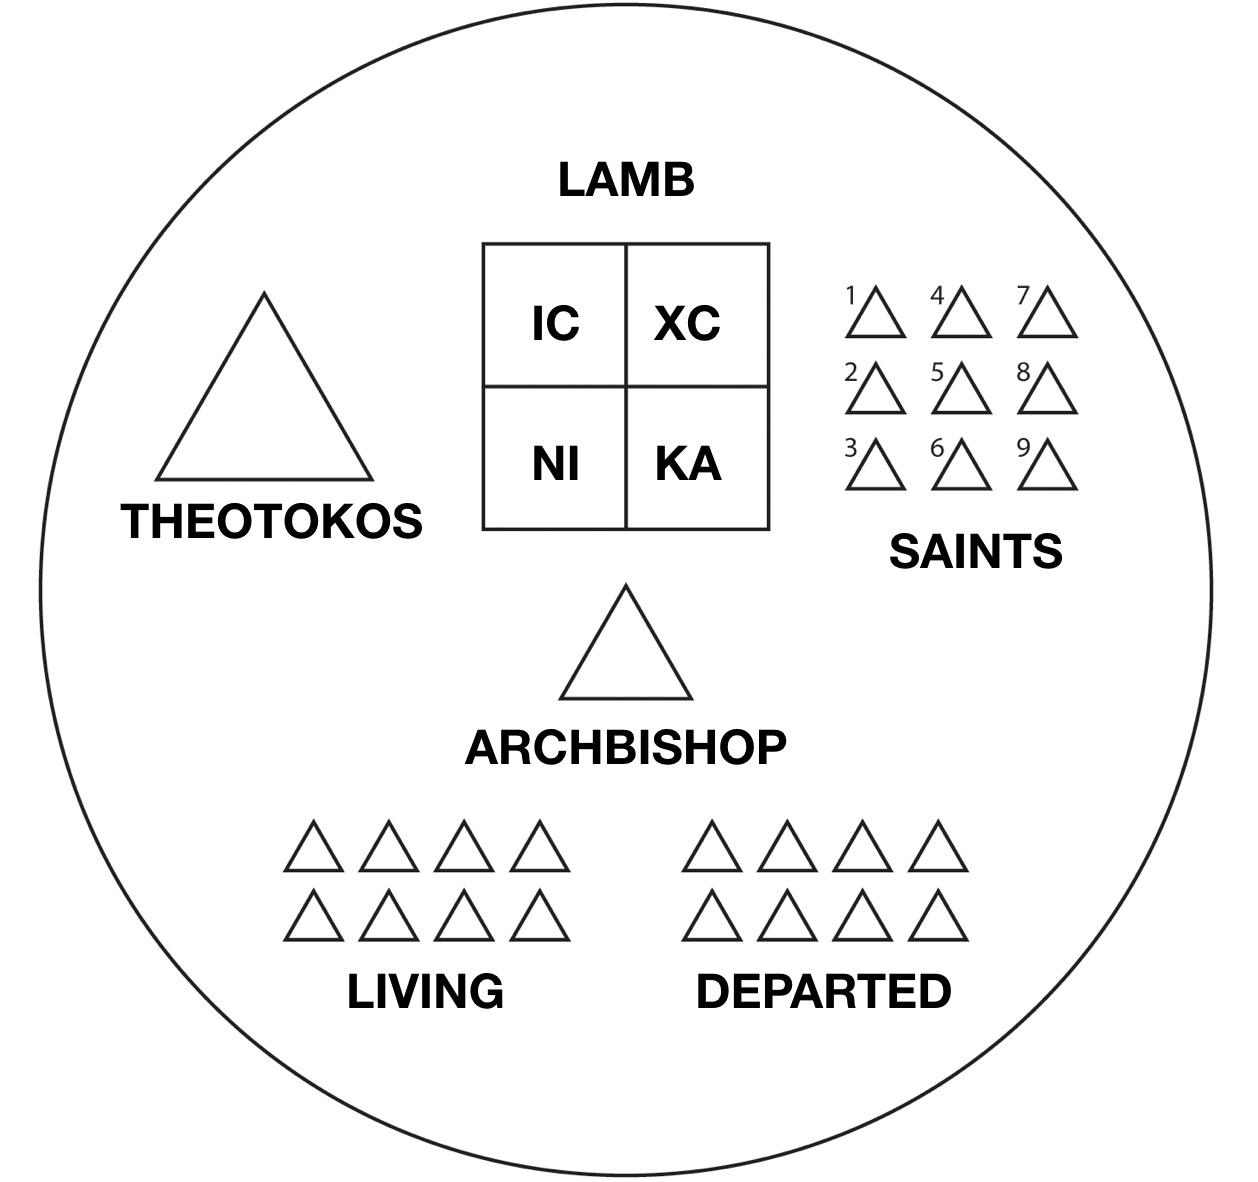
\includegraphics[scale=.15]{system/images/PriestDiagramEnglish.jpg}
\end{center}

\ltRubric{duplicates}{d1233}

\ltDialogRubricDialog{duplicates}{d0807}{duplicates}{name}{duplicates}{d0807b}

\ltRubric{duplicates}{d0984}

\ltDialogRubric{duplicates}{d0806}{duplicates}{name2}

\ltRubric{duplicates}{d0985}

\ltDialog{duplicates}{d0306}

\ltRubric{duplicates}{d1033}

\ltDialogRubric{duplicates}{d0806}{duplicates}{name2}

\ltRubric{duplicates}{d1234}

\ltDialog{duplicates}{d0118}

\ltRubric{duplicates}{d0556}

\ltRubric{duplicates}{d0284}

\ltDialog{duplicates}{d0805}

\ltRubric{duplicates}{d0888}

\ltDialog{duplicates}{d0602}

\ltRubric{duplicates}{d0916}

\ltDialog{duplicates}{d1236}

\ltActorDialog{actors}{Deacon}{duplicates}{d0593}

\ltRubric{duplicates}{d0922}

\ltDialog{duplicates}{d1237}

\ltActorDialog{actors}{Deacon}{duplicates}{d0594}

\ltRubric{duplicates}{d1238}

\ltDialog{duplicates}{d1239}

\ltActorDialog{actors}{Deacon}{duplicates}{d0247}

\ltRubric{duplicates}{d1240}


\ltDialog{duplicates}{d1179}

\ltActorDialog{actors}{Deacon}{duplicates}{d0828}

\ltRubric{duplicates}{d0924}

\ltDialog{duplicates}{d0827}

\ltRubric{duplicates}{d1008}

\ltDialog{duplicates}{d0200}

\ltRubric{duplicates}{d0267}

\ltDialog{duplicates}{d0097}

\ltRubric{duplicates}{d0137}

\ltRubric{duplicates}{d1241}

\ltDialog{duplicates}{d1242}

\ltRubric{duplicates}{d1243}

\ltSubSection{duplicates}{prayer.offertory.title}

\ltDialog{duplicates}{d0422}

\ltDialog{duplicates}{d0422b}

\ltRubric{duplicates}{d0055}

\vfill

\ltDialog{duplicates}{d0405}

\ltActorDialog{actors}{Deacon}{pub.priest.servicebook}{doxapatrikainyn}

\ltDialogRubricDialog{duplicates}{d0575}{rubrical}{Thrice}{prayers}{res13}

\ltRubricDialog{duplicates}{d0131b}{duplicates}{d0005}

\ltActorDialog{actors}{Deacon}{prayers}{res04}

\ltRubric{duplicates}{d0052}

\ltDialog{duplicates}{d1155}

\ltRubricDialog{duplicates}{d0109}{duplicates}{d1244}

\ltRubric{duplicates}{d0620}

\ltSubSection{duplicates}{li.preliminaries.title}

\ltRubric{duplicates}{d1115}

\ltRubricDialogRubric{duplicates}{leftParen}{duplicates}{d0461}{duplicates}{rightParen}

\ltRubric{duplicates}{d1029}

\ltDialogRubric{duplicates}{d0381}{rubrical}{Thrice}

\vfill

\ltDialogRubric{duplicates}{d1245}{rubrical}{Twice}

\ltRubric{duplicates}{d0877}

\ltDialog{duplicates}{d1246}{duplicates}{d1247}

\ltRubric{duplicates}{d0951}

\ltDialog{duplicates}{d0195}

\ltActorDialog{actors}{Deacon}{prayers}{res04}{duplicates}{d1248}

\ltActorDialog{actors}{Priest}{duplicates}{d1249}

\ltActorDialog{actors}{Deacon}{eu.lichrysbasil}{euLI.Key1122.text}

\ltActorDialog{actors}{Priest}{eu.lichrysbasil}{euLI.Key0106.text}

\ltActorDialog{actors}{Deacon}{prayers}{res04}

\ltRubric{duplicates}{d1005}

\vfill


%\ltChapter{pub.priest.servicebook}{li.liturgy.title}

\ltSection{pub.priest.servicebook}{li.liturgycatechumens.title}

\ltRubricDialog{pub.priest.servicebook}{li.rubric.liturgy.deacon.start}{pub.priest.servicebook}{li.bless}

\ltRubricDialog{pub.priest.servicebook}{li.rubric.beginliturgy}{prayers}{enarxis02}

\ltActorDialog{actors}{People}{prayers}{res04}

 \ltSubSection{pub.priest.servicebook}{li.litanypeace.title}

 \ltActorDialog{actors}{Deacon}{prayers}{pet01} 

 \ltActorDialogRubric{actors}{People}{prayers}{res01}
 {pub.priest.servicebook}{li.rubric.eachpetition} 

 \ltActorDialog{actors}{Deacon}{prayers}{pet02} 

\ltDialog{prayers}{pet03}

\ltDialog{prayers}{pet04}

\ltDialog{prayers}{pet06} 

\ltDialog{prayers}{pet07S}

\ltDialog{prayers}{pet08}

\ltDialog{prayers}{pet09}

\ltDialog{prayers}{pet10}

\ltDialog{prayers}{pet11}

\ltDialog{prayers}{pet12}

\ltDialog{prayers}{pet13}

\ltActorDialog{actors}{People}{prayers}{res03} 

\ltSubSection{pub.priest.servicebook}{li.prayerantifon1.title}

\ltActorDialogLowVoice{actors}{Priest}{eu.lichrysbasil}{euLI.Key0201.text} 

\ltDialogAloud{prayers}{exc01}

\ltActorDialog{actors}{People}{prayers}{res04} 

\ltSubSection{pub.priest.servicebook}{li.antifon1.title}

\ltRubric{pub.priest.servicebook}{li.rubric.iffeast}

\ltRubric{pub.priest.servicebook}{li.rubric.sundayantifon1} 

\ltDesignation{pub.priest.servicebook}{li.rubric.verseantifon1}

\ltStichos{misc}{vVerse1}{ps}{psa102.v1.text}{ps}{psa102.v1.number}

\ltActorHymn{actors}{People}{ho.s07}{hoLI.Antiphon1.text}

\ltStichos{misc}{vVerse2}{ps}{psa102.v2.text}{ps}{psa102.v2.number}

\ltActorHymn{actors}{People}{ho.s07}{hoLI.Antiphon1.text}

\ltStichos{misc}{vVerse3}{ps}{psa102.v19.text}{ps}{psa102.v19.number} 

\ltActorHymn{actors}{People}{ho.s07}{hoLI.Antiphon1.text} 

\ltStichos{misc}{vVerse4}{ps}{psa102.v22.text}{ps}{psa102.v22.number}

\ltDialog{prayers}{DoxaPatri.text}{prayers}{KaiNynKaiAei.text} 

\ltActorHymn{actors}{People}{ho.s07}{hoLI.Antiphon1.text}

\ltRubric{pub.priest.servicebook}{li.rubric.deaconpositionantifon1} 

\ltRubric{pub.priest.servicebook}{li.rubric.deaconlitany}

\ltSubSection{pub.priest.servicebook}{li.smalllitany.title}

\ltActorDialog{actors}{Deacon}{prayers}{pet14} 

\ltActorDialog{actors}{People}{prayers}{res01} 

\ltActorDialog{actors}{Deacon}{prayers}{pet12} 

\ltActorDialog{actors}{People}{prayers}{res01}

\ltActorDialog{actors}{Deacon}{prayers}{pet13} 

\ltActorDialog{actors}{People}{prayers}{res03} 

\ltSubSection{pub.priest.servicebook}{li.prayerantifon2.title}

\ltActorDialogLowVoice{actors}{Priest}{eu.lichrysbasil}{euLI.Key0301.text}

\ltDialogAloud{prayers}{exc02} 

\ltActorDialog{actors}{People}{prayers}{res04} 

\ltSubSection{pub.priest.servicebook}{li.antifon2.title}

\ltRubric{pub.priest.servicebook}{li.rubric.sundayantifon2} 

\ltRubric{pub.priest.servicebook}{li.rubric.verseantifon2} 

\ltAsterisksLine

\ltRubricHymn{pub.priest.servicebook}{li.rubric.notsunday}{me.m10.d28}{alt1.meLI.Antiphon2.text}

\ltAsterisksLine 

\ltStichos{misc}{vVerse1}{ps}{psa145.v1.text}{ps}{psa145.v2.text}{ps}{psa145.v1.number} 

\ltActorHymn{actors}{People}{ho.s07}{hoLI.Antiphon2.text} 

\ltStichos{misc}{vVerse2}{ps}{psa145.v5.text}{ps}{psa145.v5.number} 

\ltActorHymn{actors}{People}{ho.s07}{hoLI.Antiphon2.text} 

\ltStichos{misc}{vVerse3}{ps}{psa145.v6.text}{ps}{psa145.v6.number} 

\ltActorHymn{actors}{People}{ho.s07}{hoLI.Antiphon2.text} 

\ltStichos{misc}{vVerse4}{ps}{psa145.v10.text}{ps}{psa145.v10.number} 

\ltActorHymn{actors}{People}{ho.s07}{hoLI.Antiphon2.text} 

\ltDialog{prayers}{DoxaPatri.text}

\ltRubricDialog{pub.priest.servicebook}{li.rubric.alldays}{prayers}{KaiNynKaiAei.text}

\ltHymn{ho.s07}{hoLI.OnlyBegotten.text} 

\ltRubric{pub.priest.servicebook}{li.rubric.deaconpositionantifon2} 

\ltSubSection{pub.priest.servicebook}{li.smalllitany.title}

\ltActorDialog{actors}{Deacon}{prayers}{pet14} 

\ltActorDialog{actors}{People}{prayers}{res01} 

\ltActorDialog{actors}{Deacon}{prayers}{pet12} 

\ltActorDialog{actors}{People}{prayers}{res01} 

\ltActorDialog{actors}{Deacon}{prayers}{pet13} 

\ltActorDialog{actors}{People}{prayers}{res03} 

\ltSubSection{pub.priest.servicebook}{li.prayerantifon3.title}

\ltActorDialogLowVoice{actors}{Priest}{eu.lichrysbasil}{euLI.Key0401.text} 

\ltDialogAloud{prayers}{exc03}

\ltActorDialog{actors}{People}{prayers}{res04} 

\ltRubric{pub.priest.servicebook}{li.rubric.entersouth}

\ltSubSection{pub.priest.servicebook}{li.antifon3.title}

\ltRubric{pub.priest.servicebook}{li.rubric.sundayantifon3} 

\ltDesignation{pub.priest.servicebook}{li.rubric.verseantifon3}

\ltStichos{misc}{vVerse1}{ps}{psa117.v1.text}{ps}{psa117.v1.number} 

\ltRubric{pub.priest.servicebook}{li.rubric.resurrectionmode}

\ltStichos{misc}{vVerse2}{ps}{psa117.v4.text}{ps}{psa117.v4.number}

\ltRubric{pub.priest.servicebook}{li.rubric.resurrection} 

\ltStichos{misc}{vVerse3}{ps}{psa117.v24.text}{ps}{psa117.v24.number}

\ltRubric{pub.priest.servicebook}{li.rubric.resurrection} 

\ltRubric{pub.priest.servicebook}{li.rubric.smallentrance} 

\ltRubricDialog{pub.priest.servicebook}{li.rubric.deaconquietly}{prayers}{pet00}

\ltSubSection{pub.priest.servicebook}{li.prayerentrance.title}

\ltActorDialogLowVoice{actors}{Priest}{eu.lichrysbasil}{euLI.Key0501.text}

\ltDialog{prayers}{exc01}{prayers}{res04}

\ltRubricDialog{pub.priest.servicebook}{li.rubric.deaconquietly2}{eu.lichrysbasil}{euLI.Key0502.text} 

\ltRubricDialog{pub.priest.servicebook}{li.rubric.blessentrance}{eu.lichrysbasil}{euLI.Key0503.text}{prayers}{res04}

\ltRubricDialog{pub.priest.servicebook}{li.rubric.kissgospel}{prayers}{exc17}{prayers}{exc18}

\ltRubric{pub.priest.servicebook}{li.rubric.completeentrance} 

\ltRubric{pub.priest.servicebook}{li.rubric.entrancechant} 

\ltHymn{ho.s07}{hoLI.EntranceHymn.text}{ho.s07}{hoLI.Antiphon21.text}{ho.s07}{hoLI.Antiphon2s.text}{ho.s07}{hoLI.Antiphon22.text} 

\ltAsterisksLine 

\ltRubricHymn{pub.priest.servicebook}{li.rubric.notsunday}{me.m10.d28}{alt1.meLI.Antiphon2.text} 

\ltRubricHymn{pub.priest.servicebook}{li.rubric.sundaysofpascha}{ps}{psa67.v27.text}{ho.s07}{hoLI.Antiphon2.text}

\ltAsterisksLine

\ltRubric{pub.priest.servicebook}{li.rubric.kontakion1}

\ltRubric{prayers}{DoxaPatri.text}{prayers}{KaiNynKaiAei.text}

\ltRubric{pub.priest.servicebook}{li.rubric.kontakion2}

\ltRubric{pub.priest.servicebook}{li.rubric.theotokoskontakion} 

\ltHymn{ho.s07}{hoTY.Key0408.text} 

\ltRubricDialog{pub.priest.servicebook}{li.rubric.kontakion3}{prayers}{pet00}

\ltActorDialog{actors}{People}{prayers}{res01}

\ltSubSection{pub.priest.servicebook}{li.trisagionprayer.title}

\ltActorDialogLowVoice{actors}{Priest}{eu.lichrysbasil}{euLI.Key0601.text} 

\ltActorDialog{rubrical}{Aloud}{prayers}{exc05a} 

\ltRubricDialog{pub.priest.servicebook}{li.rubric.deaconkainyn}{prayers}{exc05b}

\ltActorDialog{actors}{People}{prayers}{res04} 

\ltHymn{ho.s07}{hoLI.TrisagiosHymn.text} 

\ltHymn{ho.s07}{hoLI.TrisagiosHymn.text} 

\ltHymn{ho.s07}{hoLI.TrisagiosHymn.text} 

\ltVerse{pub.priest.servicebook}{doxapatrikainyn} 

\ltHymnLastLine{ho.s07}{hoLI.TrisagiosHymn3.text}{ho.s07}{hoLI.TrisagiosHymn4.text} 

\ltActorDialog{actors}{Deacon}{eu.lichrysbasil}{euLI.Key0602.text} 

\ltActorHymn{actors}{People}{ho.s07}{hoLI.TrisagiosHymn.text} 

\ltRubric{pub.priest.servicebook}{li.rubric.trisagionclergy} 

\ltRubricDialog{pub.priest.servicebook}{li.rubric.command}{prayers}{KelefsonDespota} 

\ltRubricDialogLowVoice{pub.priest.servicebook}{li.rubric.approachthrone}{ps}{psa117.v26a.text} 

\ltActorDialogLowVoice{actors}{Deacon}{eu.lichrysbasil}{euLI.Key0605.text} 

\ltActorDialogLowVoice{actors}{Priest}{eu.lichrysbasil}{euLI.Key0606.text}

\ltSubSection{pub.priest.servicebook}{li.readings.title}

\ltActorDialog{actors}{PriestOrDeacon}{prayers}{exc19} 

\ltActorDialog{actors}{Priest}{prayers}{pet31}

\ltActorDialog{actors}{People}{prayers}{res05} 

\ltActorDialog{actors}{PriestOrDeacon}{prayers}{exc17}

\ltRubricDialog{pub.priest.servicebook}{li.rubric.prokimenontitle}{pub.priest.servicebook}{li.prokimenonmode}

\ltActorDialog{actors}{PriestOrDeacon}{prayers}{exc19}

\ltRubric{pub.priest.servicebook}{li.rubric.declaimprokimenon} 

\ltActorDialog{actors}{PriestOrDeacon}{prayers}{exc17}

\ltRubric{rubrical}{cl.eu.lichrysbasil.R009}

\ltActorDialog{actors}{PriestOrDeacon}{prayers}{exc19} 
\ltRubric{rubrical}{cl.eu.lichrysbasil.R010} 

\ltActorDialog{actors}{Priest}{prayers}{epi02} 

\ltActorDialogRubric{actors}{Chanters}{prayers}{Allilouia3.text}{pub.priest.servicebook}{li.rubric.withverses} 

\ltRubric{pub.priest.servicebook}{li.rubric.censeapostolos} 

\ltSubSection{pub.priest.servicebook}{li.gospelprayer.title}

\ltActorDialogLowVoice{actors}{Priest}{eu.lichrysbasil}{euLI.Key0704.text}

\ltRubricDialog{pub.priest.servicebook}{li.rubric.blessreader}{pub.priest.servicebook}{li.blessreader}

\ltRubricDialog{pub.priest.servicebook}{li.rubric.blessreader2}{pub.priest.servicebook}{li.blessreader2}

\ltRubricDialogRubric{pub.priest.servicebook}{li.rubric.givegospel}{prayers}{res04}{pub.priest.servicebook}{li.rubric.gospelambon} 

\ltSubSection{pub.priest.servicebook}{li.gospel.title}

\ltActorDialog{actors}{Priest}{prayers}{listen.to.holy.gospel}

\ltActorDialog{actors}{People}{prayers}{res05} 

\ltActorDialog{actors}{Deacon}{rubrical}{cl.eu.lichrysbasil.R011}

\ltActorDialog{actors}{People}{prayers}{DoxaSoiKyrie} 

\ltActorDialog{actors}{Priest}{prayers}{exc19}

\ltRubric{pub.priest.servicebook}{li.rubric.readgospel} 

\ltActorDialog{actors}{Priest}{prayers}{gos04} 

\ltActorDialog{actors}{People}{prayers}{DoxaSoiKyrie}

\ltRubric{pub.priest.servicebook}{li.rubric.blesswithgospel} 

\ltSubSection{pub.priest.servicebook}{li.kerygma.title}

\ltRubric{pub.priest.servicebook}{li.rubric.preach} 

\ltRubric{pub.priest.servicebook}{li.rubric.beginlitany}

\ltSubSection{pub.priest.servicebook}{li.greatlitany.title}

\ltActorDialog{actors}{Deacon}{prayers}{pet15}

\ltActorDialog{actors}{People}{prayers}{res01} 

\ltActorDialog{actors}{Deacon}{prayers}{pet16} 

\ltActorDialog{actors}{People}{prayers}{res01}

\ltActorDialog{actors}{Deacon}{prayers}{pet17} 

\ltActorDialogRubric{actors}{People}{prayers}{res01}{pub.priest.servicebook}{li.rubric.thriceeach}

\ltActorDialogRubricDialog{actors}{Deacon}{pub.priest.servicebook}{li.pet19lash.a}{rubrical}{name}{pub.priest.servicebook}{li.pet19lash.b}

\ltDialog{pub.priest.servicebook}{li.pet21lash} 

\ltDialog{pub.priest.servicebook}{li.pet22lash} 

\ltDialog{prayers}{pet23}

\ltActorDialog{actors}{People}{prayers}{res01} 

\ltSubSection{pub.priest.servicebook}{li.ekteniaprayer.title}

\ltActorDialogLowVoice{actors}{Priest}{eu.lichrysbasil}{euLI.Key0801.text} 

\ltDialogAloud{prayers}{exc11} 

\ltActorDialog{actors}{People}{prayers}{res04} 

\ltRubric{pub.priest.servicebook}{li.rubric.catechumens}

\ltRubricDialog{pub.priest.servicebook}{li.rubric.catechumens2}{prayers}{res01}

\ltActorDialog{actors}{PriestOrDeacon}{eu.lichrysbasil}{euLI.Key0901.text}

\ltDialog{eu.lichrysbasil}{euLI.Key0902.text} 

\ltDialog{eu.lichrysbasil}{euLI.Key0903.text} 

\ltDialog{eu.lichrysbasil}{euLI.Key0904.text} 

\ltDialog{eu.lichrysbasil}{euLI.Key0905.text} 

\ltDialog{eu.lichrysbasil}{euLI.Key0906.text} 

\ltDialog{eu.lichrysbasil}{euLI.Key0907.text} 

\ltDialog{eu.lichrysbasil}{euLI.Key0908.text} 

\ltActorDialog{actors}{People}{prayers}{res03}

\ltSubSection{pub.priest.servicebook}{li.prayercatechumens.title}

\ltDesignation{pub.priest.servicebook}{li.beforeantimension.title.doc} 

\ltActorDialogLowVoice{actors}{Priest}{eu.lichrysbasil}{euLI.Key0909.text}

\ltDialogAloud{eu.lichrysbasil}{euLI.Key0910.text} 

\ltActorDialog{actors}{People}{prayers}{res04} 

\ltRubric{pub.priest.servicebook}{li.rubric.unfoldantimension} 

\ltActorDialog{actors}{Deacon}{eu.lichrysbasil}{euLI.Key0911.text}

\ltSection{pub.priest.servicebook}{li.liturgyfaithful.title}

\ltActorDialog{actors}{PriestOrDeacon}{eu.lichrysbasil}{euLI.Key0912.text}{prayers}{pet14} 

\ltActorDialog{actors}{People}{prayers}{res01}

\ltActorDialog{actors}{PriestOrDeacon}{prayers}{pet12} 

\ltActorDialog{actors}{People}{prayers}{res01} 

\ltActorDialog{actors}{PriestOrDeacon}{prayers}{exc17} 

\ltSubSection{pub.priest.servicebook}{li.prayer1faithful.title}

\ltDesignation{pub.priest.servicebook}{li.afterantimension.title.doc} 

\ltActorDialogLowVoice{actors}{Priest}{eu.lichrysbasil}{euLI.Key1001.text}

\ltDialogAloud{prayers}{exc01} 

\ltActorDialog{actors}{People}{prayers}{res04}

\ltActorDialog{actors}{PriestOrDeacon}{prayers}{pet14} 

\ltActorDialog{actors}{People}{prayers}{res01} 

\ltActorDialog{actors}{PriestOrDeacon}{prayers}{pet12}

\ltActorDialog{actors}{People}{prayers}{res01} 

\ltActorDialog{actors}{PriestOrDeacon}{prayers}{exc17} 

\ltRubric{pub.priest.servicebook}{li.rubric.prayer2faithful}

\ltSubSection{pub.priest.servicebook}{li.prayer2faithful.title}

\ltActorDialogLowVoice{actors}{Priest}{eu.lichrysbasil}{euLI.Key1002.text}

\ltDialogAloud{eu.lichrysbasil}{euLI.Key1003.text}

\ltActorDialog{actors}{People}{prayers}{res04}

\ltSubSection{pub.priest.servicebook}{li.cherubic.title}

\ltRubric{pub.priest.servicebook}{li.rubric.cherubic} 

\ltHymn{eu.lichrysbasil}{euLI.Key1102.text} 

\ltRubric{pub.priest.servicebook}{li.rubric.prayercherubic} 

\ltSubSection{pub.priest.servicebook}{li.prayercherubic.title}

\ltDialog{eu.lichrysbasil}{euLI.Key1101.text.a}

\ltDialog{eu.lichrysbasil}{euLI.Key1101.text.b}

\ltDialog{eu.lichrysbasil}{euLI.Key1101.text.c}

\ltRubric{pub.priest.servicebook}{li.rubric.prayercherubicsecret} 

\ltActorDialog{actors}{Priest}{eu.lichrysbasil}{euLI.Key1102.text}

\ltActorDialog{actors}{PriestOrDeacon}{pub.priest.servicebook}{li.cherubic2} 

\ltRubric{pub.priest.servicebook}{li.rubric.censeatcherubikon} 

\ltRubric{pub.priest.servicebook}{li.rubric.anastasin}{ho.s03}{hoMA.SunPostGospel.text}{pub.priest.servicebook}{li.rubric.IfItIsSunday}

\ltRubric{pub.priest.servicebook}{li.rubric.IfItIsNotSunday}

\ltRubric{pub.priest.servicebook}{li.rubric.AfterPsalm50}

\ltRubricDialog{pub.priest.servicebook}{li.rubric.approachprothesis}{pub.priest.servicebook}{li.preparation.mercy}

\ltRubricDialog{pub.priest.servicebook}{li.rubric.eparon}{pub.priest.servicebook}{li.eparon} 

\ltRubricDialogRubric{pub.priest.servicebook}{li.rubric.wearaer}{ps.kenya.alt}{psa133.v2alt2.text}{pub.priest.servicebook}{li.rubric.psa133.v2.fullattribution}

\ltRubric{pub.priest.servicebook}{li.rubric.takegifts} 

\ltRubric{pub.priest.servicebook}{li.rubric.procession} 

\ltDialog{eu.lichrysbasil}{euLI.Key1110.text}

\ltActorDialog{actors}{Chanter}{prayers}{res04} 

\ltRubric{pub.priest.servicebook}{li.rubric.completehymn} 

\ltHymn{pub.priest.servicebook}{li.cherubic2} 

\ltRubric{pub.priest.servicebook}{li.rubric.enteraltar} 

\ltRubricDialogLowVoice{pub.priest.servicebook}{li.rubric.deaconright}{eu.lichrysbasil}{euLI.Key1114.text}

\ltRubricDialogLowVoice{pub.priest.servicebook}{li.rubric.priestresponse}{pub.priest.servicebook}{li.holydiaconate}

\ltRubricDialogLowVoice{pub.priest.servicebook}{li.rubric.placegiftsaltar}{pub.priest.servicebook}{li.noblejoseph}

\ltRubric{pub.priest.servicebook}{li.rubric.covergiftsaer} 

\ltDialog{eu.lichrysbasil}{euLI.Key1116.text} 

\ltActorDialogLowVoiceRubric{actors}{Priest}{ps}{psa50.v20.v21.a.and.b}{pub.priest.servicebook}{li.rubric.psa50.v20.v21.fullattribution} 

\ltRubricDialogLowVoice{pub.priest.servicebook}{li.rubric.rememberpriest}{eu.lichrysbasil}{euLI.Key1118.text}

\ltActorDialogLowVoice{actors}{Deacon}{eu.lichrysbasil}{euLI.Key1114.text}

\ltActorDialogLowVoice{actors}{Priest}{pub.priest.servicebook}{li.praypriest} 

\ltActorDialogLowVoice{actors}{Deacon}{eu.lichrysbasil}{euLI.Key1120.text}

\ltActorDialogLowVoice{actors}{Priest}{eu.lichrysbasil}{euLI.Key1121.text}

\ltRubricDialogLowVoice{pub.priest.servicebook}{li.rubric.rememberdeacon}{eu.lichrysbasil}{euLI.Key1122.text}

\ltActorDialogLowVoice{actors}{Priest}{eu.lichrysbasil}{euLI.Key0106.text}

\ltRubricDialogRubric{pub.priest.servicebook}{li.rubric.andsaying}{prayers}{res04}{pub.priest.servicebook}{li.rubric.beginlitanygifts}

\ltSubSection{pub.priest.servicebook}{li.litanygifts.title}

\ltActorDialog{actors}{PriestOrDeacon}{prayers}{pet24}

\ltActorDialogRubric{actors}{People}{prayers}{res01}{pub.priest.servicebook}{li.rubric.eachpetition2}

\ltActorDialog{actors}{PriestOrDeacon}{eu.lichrysbasil}{euLI.Key1201.text}

\ltDialog{prayers}{pet04}

\ltDialog{prayers}{pet11}

\ltDialog{prayers}{pet12}

\ltDialog{prayers}{pet25m}

\ltActorDialogRubric{actors}{People}{prayers}{res02}{pub.priest.servicebook}{li.rubric.eachpetition2}

\ltActorDialog{actors}{PriestOrDeacon}{prayers}{pet26} 

\ltDialog{prayers}{pet27}

\ltDialog{prayers}{pet28}

\ltDialog{prayers}{pet29}

\ltDialog{prayers}{pet30}

\ltDialog{prayers}{pet13}

\ltActorDialog{actors}{People}{prayers}{res03} 

\ltSubSection{eu.lichrysbasil}{euLI.Key1202.title}

\ltActorDialogLowVoice{actors}{Priest}{eu.lichrysbasil}{euLI.Key1202.text} 

\ltDialogAloud{eu.lichrysbasil}{euLI.Key1203.text}

\ltActorDialog{actors}{People}{prayers}{res04} 

\ltActorDialog{actors}{Priest}{prayers}{pet31} 

\ltActorDialog{actors}{People}{prayers}{res05} 

\ltActorDialog{actors}{Deacon}{eu.lichrysbasil}{euLI.Key1204.text}

\ltActorHymn{actors}{People}{eu.lichrysbasil}{euLI.Key1205.text}

\ltRubricDialog{pub.priest.servicebook}{li.rubric.agapwse}{ps}{psa17.v2.text}{ps}{psa17.v3a.text}

\ltRubric{pub.priest.servicebook}{li.rubric.kissofpeace}

\ltRubric{pub.priest.servicebook}{li.rubric.deaconkiss} 

\ltSubSection{pub.priest.servicebook}{li.creed.title}

\ltActorDialog{actors}{Deacon}{eu.lichrysbasil}{euLI.Key1208.text}
\ltActorReading{actors}{People}{prayers}{Pistevo.text.a} 
\ltReading{prayers}{Pistevo.text.b}

\ltReading{prayers}{Pistevo.text.c}

\ltReading{prayers}{Pistevo.text.d}

\ltRubric{pub.priest.servicebook}{li.rubric.waveaer}

\ltSubSection{eu.lichrysbasil}{euLI.Key1300.title}

\ltActorDialog{actors}{PriestOrDeacon}{eu.lichrysbasil}{euLI.Key1301.text}

\ltActorDialog{actors}{People}{eu.lichrysbasil}{euLI.Key1302.text}

\ltRubric{pub.priest.servicebook}{li.rubric.deaconreturn} 

\ltActorRubricDialog{actors}{Priest}{pub.priest.servicebook}{li.rubric.priestblessing}{eu.lichrysbasil}{euLI.Key1303.text}

\ltActorDialog{actors}{People}{eu.lichrysbasil}{euLI.Key1304.text}

\ltActorRubricDialog{actors}{Priest}{pub.priest.servicebook}{li.rubric.liftinghands}{eu.lichrysbasil}{euLI.Key1305.text} 

\ltActorDialog{actors}{People}{eu.lichrysbasil}{euLI.Key1306.text}

\ltActorDialog{actors}{Priest}{eu.lichrysbasil}{euLI.Key1307.text}

\ltActorDialog{actors}{People}{eu.lichrysbasil}{euLI.Key1308.text}

\ltActorDialogLowVoice{actors}{Priest}{eu.lichrysbasil}{euLI.Key1309.text}

\ltDialogAloud{eu.lichrysbasil}{euLI.Key1310.text} 

\ltActorHymn{actors}{People}{eu.lichrysbasil}{euLI.Key1311.text}

\ltRubric{pub.priest.servicebook}{li.rubric.removestar} 

\ltActorDialogLowVoice{actors}{Priest}{eu.lichrysbasil}{euLI.Key1312.text}

\ltDialogAloud{eu.lichrysbasil}{euLI.Key1313.text} 

\ltActorDialog{actors}{People}{prayers}{res04}

\ltActorDialogLowVoice{actors}{Priest}{eu.lichrysbasil}{euLI.Key1314.text}

\ltActorDialog{rubrical}{Aloud}{eu.lichrysbasil}{euLI.Key1315.text}

\ltActorDialog{actors}{People}{prayers}{res04}

\ltActorDialogLowVoice{actors}{Priest}{eu.lichrysbasil}{euLI.Key1316.text}

\ltRubric{pub.priest.servicebook}{li.rubric.exaltgifts} 

\ltActorDialogAloud{actors}{Priest}{pub.priest.servicebook}{li.tasa}

\ltActorHymn{actors}{People}{pub.priest.servicebook}{li.seimnumen}

\ltRubricDialogLowVoice{pub.priest.servicebook}{li.rubric.bowinghead}{eu.lichrysbasil}{euLI.Key1319.text}

\ltRubricDialogLowVoice{pub.priest.servicebook}{li.rubric.pointbread}{pub.priest.servicebook}{li.changebread}

\ltRubricDialog{pub.priest.servicebook}{li.rubric.changebread}{eu.lichrysbasil}{euLI.Key1321.text}

\ltActorDialogLowVoice{actors}{Deacon}{prayers}{res04}

\ltRubricDialogLowVoice{pub.priest.servicebook}{li.rubric.pointchalice}{pub.priest.servicebook}{li.changewine} 

\ltRubricDialog{pub.priest.servicebook}{li.rubric.blesschalice}{eu.lichrysbasil}{euLI.Key1323.text}

\ltActorDialogLowVoice{actors}{Deacon}{prayers}{res04} 

\ltRubricDialogLowVoice{pub.priest.servicebook}{li.rubric.blessboth}{pub.priest.servicebook}{li.blessboth}

\ltRubricDialog{pub.priest.servicebook}{li.rubric.epiclesis}{eu.lichrysbasil}{euLI.Key1325.text}

\ltActorDialogLowVoice{actors}{Deacon}{prayers}{res10}

\ltRubricDialogLowVoice{pub.priest.servicebook}{li.rubric.forvigilance}{eu.lichrysbasil}{euLI.Key1326.text}

\ltRubricDialog{pub.priest.servicebook}{li.rubric.censemegalynarion}{eu.lichrysbasil}{euLI.Key1327.text}

\ltActorHymn{actors}{Chanter}{prayers}{AxionEstin.text}

\ltAsterisksLine

\ltRubric{pub.priest.servicebook}{li.rubric.megalynarionfeast} 

\ltAsterisksLine

\ltRubric{pub.priest.servicebook}{li.rubric.censecommemmorate} 

\ltDialogLowVoice{eu.lichrysbasil}{euLI.Key1329.text.a}

\ltDialog{eu.lichrysbasil}{euLI.Key1329.text.b}

\ltDialog{eu.lichrysbasil}{euLI.Key1329.text.c}

\ltDialog{eu.lichrysbasil}{euLI.Key1329.text.d}

\ltActorDialogAloud{actors}{Clergy}{client}{euLI.Key1330.text}%

\ltRubricDialog{pub.priest.servicebook}{li.rubric.wote}{eu.lichrysbasil}{euLI.Key1331.text}

\ltActorDialog{actors}{People}{eu.lichrysbasil}{euLI.Key1332.text}

\ltActorDialogLowVoice{actors}{Priest}{eu.lichrysbasil}{euLI.Key1333.text}

\ltDialogAloud{eu.lichrysbasil}{euLI.Key1334.text} 

\ltActorDialog{actors}{People}{prayers}{res04}

\ltRubricDialog{pub.priest.servicebook}{li.rubric.blessmercy}{eu.lichrysbasil}{euLI.Key1335.text}

\ltActorDialog{actors}{People}{eu.lichrysbasil}{euLI.Key1336.text}

\ltSubSection{pub.priest.servicebook}{li.litanylordsprayer.title}

\ltRubric{pub.priest.servicebook}{li.rubric.litanylords} 

\ltActorDialog{actors}{PriestOrDeacon}{eu.lichrysbasil}{euLI.Key1401.text}

\ltActorDialogRubric{actors}{People}{prayers}{res01}{pub.priest.servicebook}{li.rubric.eachpetition} 

\ltActorDialog{actors}{PriestOrDeacon}{eu.lichrysbasil}{euLI.Key1402.text}

\ltDialog{eu.lichrysbasil}{euLI.Key1403.text}

\ltDialog{prayers}{pet11}

\ltDialog{prayers}{pet12}

\ltDialog{prayers}{pet25m}

\ltActorDialogRubric{actors}{People}{prayers}{res02}{pub.priest.servicebook}{li.rubric.eachpetition} 

\ltActorDialog{actors}{PriestOrDeacon}{prayers}{pet26}

\ltDialog{prayers}{pet27}

\ltDialog{prayers}{pet28} 

\ltDialog{prayers}{pet29}

\ltDialog{prayers}{pet30}

\ltDialog{eu.lichrysbasil}{euLI.Key1404.text} 

\ltActorDialog{actors}{People}{prayers}{res03} 

\ltActorDialogLowVoice{actors}{Priest}{eu.lichrysbasil}{euLI.Key1405.text}

\ltDialogAloud{eu.lichrysbasil}{euLI.Key1406.text} 

\ltSubSection{titles}{KyriakiProsefchi.title}

\ltActorReading{actors}{People}{prayers}{PaterImon.text} 

\ltActorDialogAloud{actors}{Priest}{prayers}{exc20}

\ltActorDialog{actors}{People}{prayers}{res04}

\ltActorDialog{actors}{Priest}{prayers}{pet31} 

\ltActorDialog{actors}{People}{prayers}{res05} 

\ltActorDialog{actors}{PriestOrDeacon}{prayers}{pet32} 

\ltActorDialog{actors}{People}{prayers}{res03} 

\ltActorDialogLowVoice{actors}{Priest}{eu.lichrysbasil}{euLI.Key1407.text}

\ltDialogAloud{prayers}{exc07a} 

\ltActorDialog{actors}{People}{prayers}{res04}

\ltSubSection{pub.priest.servicebook}{li.holycommunion.title}

\ltActorDialog{actors}{Priest}{eu.lichrysbasil}{euLI.Key1409.text}

\ltRubricDialogLowVoice{pub.priest.servicebook}{li.rubric.bowcommunion}{pub.priest.servicebook}{li.preparation.mercy}

\ltActorDialog{actors}{PriestOrDeacon}{prayers}{exc19}

\ltRubricDialog{pub.priest.servicebook}{li.rubric.holyforholy}{eu.lichrysbasil}{euLI.Key1410.text}

\ltActorHymn{actors}{People}{eu.lichrysbasil}{euLI.Key1411.text}

\ltRubric{pub.priest.servicebook}{li.rubric.communionhymn} 

\ltRubric{pub.priest.servicebook}{li.rubric.communionhymnsunday} 

\ltHymnRubric{ps}{psa148.v1.text}{titles}{Allilouia.title.doc}{pub.priest.servicebook}{li.rubric.communionhymnfullattribution}

\ltRubric{pub.priest.servicebook}{li.rubric.communionhymnotherdays} 

\ltRubricDialogLowVoice{pub.priest.servicebook}{li.rubric.crossorarion}{eu.lichrysbasil}{euLI.Key1501.text}

\ltRubricDialogLowVoice{pub.priest.servicebook}{li.rubric.breakbread}{eu.lichrysbasil}{euLI.Key1502.text}

\ltRubric{pub.priest.servicebook}{li.rubric.placecrosswise} 
\begin{center}
\begin{tabular}{ r c l }
   & IC &  \\
  NI &  & KA \\
   & XC &  \\
\end{tabular}
\end{center}
\ltRubricDialogLowVoice{pub.priest.servicebook}{li.rubric.fillchalice}{eu.lichrysbasil}{euLI.Key1503.text}

\ltRubricDialogLowVoice{pub.priest.servicebook}{li.rubric.ic}{pub.priest.servicebook}{li.pliroma}

\ltActorDialogLowVoice{actors}{Deacon}{prayers}{res04}

\ltRubricDialogLowVoice{pub.priest.servicebook}{li.rubric.takezeon}{eu.lichrysbasil}{euLI.Key1505.text}

\ltRubricDialogLowVoice{pub.priest.servicebook}{li.rubric.blesszeon}{eu.lichrysbasil}{euLI.Key1506.text}

\ltRubricDialogLowVoice{pub.priest.servicebook}{li.rubric.pourzeon}{pub.priest.servicebook}{li.zesis}

\ltRubricDialogLowVoice{pub.priest.servicebook}{li.rubric.approachbody}{eu.lichrysbasil}{euLI.Key1509.text}

\ltRubricDialogLowVoice{pub.priest.servicebook}{li.rubric.xc}{eu.lichrysbasil}{euLI.Key1510.text}

\ltRubricDialogLowVoice{pub.priest.servicebook}{li.rubric.wipehand}{pub.priest.servicebook}{li.deaconcommune}

\ltRubricDialogLowVoice{pub.priest.servicebook}{li.rubric.deaconcommune}{eu.lichrysbasil}{euLI.Key1512.text}

\ltRubricDialogLowVoice{pub.priest.servicebook}{li.rubric.deaconcommune2}{eu.lichrysbasil}{euLI.Key1513.text}

\ltRubric{pub.priest.servicebook}{li.rubric.deaconcommune3} 

\ltRubricDialogLowVoice{pub.priest.servicebook}{li.rubric.chaliceandcloth}{eu.lichrysbasil}{euLI.Key1515.text}

\ltRubricDialogLowVoice{pub.priest.servicebook}{li.rubric.drinkthrice}{eu.lichrysbasil}{euLI.Key1516.text}

\ltRubricDialogLowVoice{pub.priest.servicebook}{li.rubric.deaconcommune4}{pub.priest.servicebook}{li.deaconcommune2}

\ltRubricDialogLowVoice{pub.priest.servicebook}{li.rubric.deaconcommune5}{pub.priest.servicebook}{li.approachagain}{eu.lichrysbasil}{euLI.Key1518.text}

\ltRubricDialogLowVoice{pub.priest.servicebook}{li.rubric.chaliceandcloth}{pub.priest.servicebook}{li.etimetadidotai}

\ltRubricDialogLowVoice{pub.priest.servicebook}{li.rubric.deaconcommune6}{eu.lichrysbasil}{euLI.Key1520.text}

\ltRubric{pub.priest.servicebook}{li.rubric.nika} 

\ltSubSection{pub.priest.servicebook}{li.distribution.title}

\ltRubricDialog{pub.priest.servicebook}{li.rubric.approach}{eu.lichrysbasil}{euLI.Key1526.text}

\ltActorDialog{actors}{People}{pub.priest.servicebook}{li.godisthelord}

\ltRubricDialog{pub.priest.servicebook}{li.rubric.distributionprayer}{pub.priest.servicebook}{li.distributionprayershort} 

\ltRubricHymn{pub.priest.servicebook}{li.rubric.toudeipnou}{ho.s21}{hoPCPrayer.TouDeipnouSou.text}

\ltAsterisksLine

\ltRubricHymn{pub.priest.servicebook}{li.rubric.paschalcommunion}{pe.d00P}{pePA.CommunionHymn.text}{pub.priest.servicebook}{li.alleluia}

\ltAsterisksLine

\ltRubric{pub.priest.servicebook}{li.rubric.replacechalice} 

\ltRubricDialog{pub.priest.servicebook}{li.rubric.blesshand}{eu.lichrysbasil}{euLI.Key1529.text}

\ltActorHymn{actors}{People}{eu.lichrysbasil}{euLI.Key1530.text}

\ltAsterisksLine

\ltRubric{pub.priest.servicebook}{li.rubric.iflordsfeast}{pub.priest.servicebook}{li.rubric.paschal} 

\ltAsterisksLine

\ltRubricDialog{pub.priest.servicebook}{li.rubric.wipeparticles}{eu.lichrysbasil}{euLI.Key1525.text}

\ltRubricDialog{pub.priest.servicebook}{li.rubric.eparon.b}{eu.lichrysbasil}{euLI.Key1601.text}

\ltRubricDialog{pub.priest.servicebook}{li.rubric.censeexalt}{ps}{psa56.v6.text}

\ltRubric{pub.priest.servicebook}{li.rubric.showcoversstar} 

\ltRubricDialogRubricDialog{pub.priest.servicebook}{li.rubric.blessed}{prayers}{EvlogitosOTheosImon.text}{pub.priest.servicebook}{li.rubric.blessed2}{prayers}{PantoteNyn.text}

\ltActorDialog{actors}{People}{prayers}{res04}

\ltActorHymn{actors}{People}{eu.lichrysbasil}{euLI.Key1603.text}

\ltSubSection{pub.priest.servicebook}{li.thanksdismissal.title}

\ltRubric{pub.priest.servicebook}{li.rubric.foldantimension} 

\ltRubricDialog{pub.priest.servicebook}{li.rubric.havingpartaken}{eu.lichrysbasil}{euLI.Key1604.text}

\ltActorDialogRubricDialog{actors}{People}{prayers}{res01}{rubrical}{Or}{prayers}{DoxaSoiKyrie} 

\ltActorDialog{actors}{PriestOrDeacon}{prayers}{pet12}

\ltActorDialog{actors}{People}{prayers}{res01} 

\ltActorDialog{actors}{PriestOrDeacon}{eu.lichrysbasil}{euLI.Key1605.text}

\ltActorDialog{actors}{People}{prayers}{res03} 

\ltSubSection{eu.lichrysbasil}{euLI.Key1606.title}

\ltActorDialogLowVoice{actors}{Priest}{eu.lichrysbasil}{euLI.Key1606.text}

\ltRubricDialog{pub.priest.servicebook}{li.rubric.crossantimensiongospel}{prayers}{exc24} 

\ltActorDialog{actors}{People}{prayers}{res04}

\ltSubSection{eu.lichrysbasil}{euLI.Key1700.title}

\ltActorDialog{actors}{Priest}{eu.lichrysbasil}{euLI.Key1701.text}

\ltActorDialog{actors}{People}{pub.priest.servicebook}{li.lordsname}

\ltActorDialog{actors}{Deacon}{prayers}{pet00} 

\ltActorDialog{actors}{People}{prayers}{res01}

\ltRubric{pub.priest.servicebook}{li.rubric.ambonprayer}

\ltSubSection{pub.priest.servicebook}{li.ambonprayer.title}

\ltActorDialog{actors}{Priest}{eu.lichrysbasil}{euLI.Key1702.text}

\ltActorHymnHymnRubric{actors}{People}{prayers}{res04}{ps}{psa112.v2alt1.text}{rubrical}{Thrice} 

\ltRubricDialog{pub.priest.servicebook}{li.rubric.pliromanomou}{eu.lichrysbasil}{euLI.Key1704.text}

\ltActorDialog{actors}{PriestOrDeacon}{prayers}{pet00} 

\ltActorDialog{actors}{People}{prayers}{res01} 

\ltRubricDialog{pub.priest.servicebook}{li.rubric.evlogiakyriou}{prayers}{pet37} 

\ltActorDialog{actors}{People}{prayers}{res04} 

\ltActorDialog{actors}{Priest}{pub.priest.servicebook}{DoxaSoiOTheos2}

\ltActorDialog{actors}{Reader}{pub.priest.servicebook}{doxapatrikainyn}{prayers}{res06}{prayers}{res13} 



\ltActorDialogRubricDialog{actors}{Priest}{pub.priest.servicebook}{li.dis.oanastas}{pub.priest.servicebook}{li.rubric.sundaydismissal}{dismissals}{combo}

\ltDialog{prayers}{DiEfchonPateron.text} 

\ltActorDialog{actors}{People}{prayers}{res04}

\ltRubricDialog{pub.priest.servicebook}{li.rubric.finalblessing}{eu.lichrysbasil}{euLI.Key1707.text}

\ltActorHymn{actors}{People}{eu.lichrysbasil}{euLI.Key1706.text}

\ltRubricDialog{pub.priest.servicebook}{li.rubric.giveantidoron}{pub.priest.servicebook}{li.blessingmercy}

\ltDesignation{pub.priest.servicebook}{li.end.title.doc} 

\vfill
\pagebreak


% Basil prayers added to liturgy

% Presanctified

% Pentecost Kneeling service

%\ltChapter{duplicates}{apolytikia.title}

\ltSection{duplicates}{apolytikia.resur.title}

\ltDesignation{duplicates}{d0488}

\ltModeMelody{misc}{Mode1}

\ltHymn{duplicates}{d0965}

\ltModeMelody{misc}{Mode2}

\ltHymn{duplicates}{d0147}

\ltModeMelody{misc}{Mode3}

\ltHymn{duplicates}{d1158}

\ltModeMelody{misc}{Mode4}

\ltHymn{duplicates}{d1162}

\ltModeMelody{misc}{Mode5}

\ltHymn{duplicates}{d0965}

\ltModeMelody{misc}{Mode6}

\ltHymn{duplicates}{d0147}

\ltModeMelody{misc}{Mode7}

\ltHymn{duplicates}{d1158}

\ltModeMelody{misc}{Mode8}

\ltHymn{duplicates}{d1162}

\ltSection{duplicates}{apolytikia.feasts.title}

\ltRubric{duplicates}{d0825}

\ltModeMelody{misc}{Mode4}

\ltHymn{duplicates}{d1177}

\ltRubric{duplicates}{d0821}

\ltModeMelody{misc}{Mode1}

\ltHymn{duplicates}{d0591}

\ltRubric{duplicates}{d0648}

\ltModeMelody{misc}{Mode4}

\ltHymn{duplicates}{d1058}

\ltRubric{duplicates}{d0964}

\ltModeMelody{misc}{Mode2}

\ltHymn{duplicates}{d1164}

\ltRubric{duplicates}{d0963}

\ltModeMelody{misc}{Mode2}

\ltHymn{duplicates}{d0429}

\ltRubric{duplicates}{d0256}

\ltModeMelody{misc}{Mode4}

\ltHymn{duplicates}{d1173}

\ltRubric{duplicates}{d0522}

\ltModeMelody{misc}{Mode1}

\ltHymn{duplicates}{d0164}

\ltRubric{duplicates}{d0282}

\ltModeMelody{misc}{Mode1}

\ltHymn{duplicates}{d0433}

\ltRubric{duplicates}{d0597}

\ltModeMelody{misc}{Mode4}

\ltHymn{duplicates}{d1057}

\ltRubric{duplicates}{d0173}

\ltModeMelody{misc}{Mode7}

\ltHymn{duplicates}{d1170}

\ltRubric{duplicates}{d0172}

\ltModeMelody{misc}{Mode1}

\ltHymn{duplicates}{d0500}

\ltSection{duplicates}{apolytikia.triodion.title}

\ltRubric{duplicates}{d0367}

\ltModeMelody{misc}{Mode2}

\ltHymn{duplicates}{d1108}

\ltRubric{duplicates}{d0703}

\ltModeMelody{misc}{Mode8}

\ltHymn{duplicates}{d0730}

\ltRubric{duplicates}{d0704}

\ltModeMelody{misc}{Mode1}

\ltHymn{duplicates}{d0591}

\ltRubric{duplicates}{d0705}

\ltModeMelody{misc}{Mode8}

\ltHymn{duplicates}{d1154}

\ltRubric{duplicates}{d0706}

\ltModeMelody{misc}{Mode8}

\ltHymn{duplicates}{d0508}

\ltRubric{duplicates}{d0693}

\ltModeMelody{misc}{Mode1}

\ltHymn{duplicates}{d0165}

\ltRubric{duplicates}{d0150}

\ltModeMelody{misc}{Mode4}

\ltHymn{duplicates}{d0215}

\ltRubric{duplicates}{d0709}

\ltModeMelody{misc}{Mode5}

\ltHymn{duplicates}{d0231}

\ltRubric{duplicates}{d0709}

\ltModeMelody{misc}{Mode5}

\ltHymn{duplicates}{d0231}

\ltRubric{duplicates}{d0715}

\ltModeMelody{misc}{Mode7}

\ltHymn{duplicates}{d1129}

\ltRubric{duplicates}{d0979}

\ltHymn{duplicates}{d0866}

\ltRubric{duplicates}{d0721}

\ltModeMelody{misc}{Mode8}

\ltHymn{duplicates}{d0168}

\ltRubric{duplicates}{d0708}

\ltModeMelody{misc}{Mode4}

\ltHymn{duplicates}{d1169}

\ltRubric{duplicates}{d0716}

\ltModeMelody{misc}{Mode8}

\ltHymn{duplicates}{d1159}

\ltRubric{duplicates}{d0714}

\ltModeMelody{misc}{Mode8}

\ltHymn{duplicates}{d0186}

\ltRubric{duplicates}{d0713}

\ltModeMelody{misc}{Mode4}

\ltHymn{duplicates}{d0238}


%\ltChapter{duplicates}{kontakia.title}

\ltRubric{duplicates}{d0823}

\ltModeMelody{misc}{Mode4}{duplicates}{d0627}

\ltHymn{duplicates}{d0596}

\ltRubric{duplicates}{d0824}

\ltModeMelody{misc}{Mode3}

\ltHymn{duplicates}{d1079}

%\ltRubric

%\ltModeMelody{misc}{Mode4}

%\ltHymn


% Ordinations
%   Reader
%   Deacon
%   Priest
%   Archimandrite
%   ProtoPresbyter / Confessor

%\ltChapter{baptism}{p0001.title}

\ltSection{baptism}{p0002.title}

\ltSubSection{eu.baptism}{euBAP.Key0101.title}%

\ltRubric{eu.baptism}{euBap.Key0101r.text}%

\ltActorDialog{actors}{Priest}{eu.baptism}{euBap.Key0101.text}%
\vfill%

\ltSubSection{eu.baptism}{euBAP.Key0103.title}%

\ltActorDialog{actors}{Deacon}{duplicates}{d0551}

\ltActorDialog{actors}{People}{duplicates}{d0575}

\ltActorDialog{actors}{Priest}{baptism}{p0026}

\ltActorDialog{actors}{People}{prayers}{res04}

\vfill%
\ltSubSection{eu.baptism}{euBAP.Key0104.title}%

\ltActorDialog{actors}{Deacon}{duplicates}{d0551}

\ltActorDialog{actors}{People}{duplicates}{d0575}

\ltActorDialog{actors}{Priest}{baptism}{p0035}

\ltActorDialog{actors}{People}{prayers}{res04}
\vfill%
\ltSubSection{eu.baptism}{euBAP.Key0105.title}%

\ltActorDialog{actors}{Deacon}{duplicates}{d0551}

\ltActorDialog{actors}{People}{duplicates}{d0575}

\ltActorDialog{actors}{Priest}{baptism}{p0044}

\ltActorDialog{actors}{People}{prayers}{res04}

\ltActorDialog{actors}{Deacon}{duplicates}{d0551}

\ltActorDialog{actors}{People}{duplicates}{d0575}

\ltActorDialog{actors}{Priest}{baptism}{p0052}

\ltRubric{baptism}{p0053}

\ltRubricDialog{rubrical}{Aloud}{baptism}{p0057}

\ltActorDialog{actors}{People}{prayers}{res04}

\ltRubric{baptism}{p0060}

\ltDialog{baptism}{p0062}

\ltRubric{baptism}{p0063}


\ltDialog{baptism}{p0064}

\ltRubric{baptism}{p0065}


\ltDialog{baptism}{p0067}

\ltRubric{duplicates}{d0125}

\ltDialog{baptism}{p0069}

\ltRubric{baptism}{p0070}

\ltDialog{baptism}{p0072}

\ltRubric{baptism}{p0073}

\ltDialog{baptism}{p0075}

\ltRubric{baptism}{p0076}

\ltDialog{baptism}{p0077}

\ltRubric{baptism}{p0078}

\ltDialog{duplicates}{d0445}

\ltRubric{baptism}{p0081}

\ltDialog{duplicates}{d0227}

\ltRubric{baptism}{p0083}

\ltDialog{baptism}{p0085}

\ltRubric{baptism}{p0086}

\ltDialogRubric{baptism}{p0087}{baptism}{p0088}

\ltDialog{baptism}{p0089}

\ltDialog{baptism}{p0090}

\ltDialog{baptism}{p0091}

\ltRubricDialogRubric{baptism}{p0092a}{duplicates}{d0445}{baptism}{p0092c}%

\ltDialog{duplicates}{d0445}

\ltRubric{duplicates}{d0125}

\ltDialog{duplicates}{d0227}

\ltRubric{baptism}{p0097}

\ltDialog{baptism}{p0099}

\ltRubric{baptism}{p0100}

\ltDialog{baptism}{p0101}

\ltRubric{baptism}{p0102}

\ltDialog{baptism}{p0103}

\ltDialog{baptism}{p0104}

\ltActorDialog{actors}{Deacon}{duplicates}{d0551}

\ltActorDialog{actors}{People}{duplicates}{d0575}

\ltActorDialogRubricDialog{actors}{Priest}{baptism}{p0110a}{baptism}{p0110b}{baptism}{p0110c}

\ltActorDialog{actors}{People}{prayers}{res04}

\ltSection{baptism}{p0113.title}

\ltRubric{baptism}{p0114}

\ltRubricDialog{duplicates}{d0995b}{duplicates}{d0607}

\ltRubricDialog{duplicates}{d0780b}{duplicates}{d0203}

\ltActorDialog{actors}{People}{prayers}{res04}

\ltActorDialog{actors}{Deacon}{duplicates}{d0504}

\ltActorDialog{actors}{People}{duplicates}{d0585}

\ltActorDialog{actors}{Deacon}{duplicates}{d0318}

\ltDialog{duplicates}{d0319}

\ltDialog{duplicates}{d0326}

\ltDialog{baptism}{p0131}

\ltDialog{baptism}{p0132}

\ltDialog{baptism}{p0133}

\ltDialog{baptism}{p0134}

\ltDialog{baptism}{p0135}

\ltDialog{baptism}{p0136}

\ltDialog{baptism}{p0137}

\ltDialog{baptism}{p0138}

\ltDialog{baptism}{p0139}

\ltDialog{baptism}{p0140}

\ltDialog{baptism}{p0141}

\ltDialog{baptism}{p0142}

\ltDialog{duplicates}{d0304}

\ltDialog{duplicates}{d0463}

\ltDialog{duplicates}{d0246}

\ltActorDialog{actors}{People}{duplicates}{d1054}

%

%\ltActor{\ltSid{"actors"}{"Priest"}}

%\ltDialog{\ltSid{"duplicates"}{"d0551"}}

%

%\ltActor{\ltSid{"actors"}{"People"}}

%\ltDialog{\ltSid{"duplicates"}{"d0575"}}

\ltRubric{baptism}{p0148}

%\ltActor{\ltSid{"actors"}{"Priest"}}

\ltDialog{baptism}{p0154}

\ltRubricDialogRubric{baptism}{p0155a}{baptism}{p0155b}{baptism}{p0155c}

\ltDialogRubricDialog{baptism}{p0157}{duplicates}{dx3}{baptism}{p0161}

\ltRubric{baptism}{p0167}

\ltDialogRubric{eu.baptism}{euBap.Key0271.text}{duplicates}{dx3}

\ltDialog{baptism}{p0171}

\ltActorDialog{actors}{People}{prayers}{res04}

\ltActorDialog{actors}{Priest}{duplicates}{d0767}

\ltActorDialog{actors}{People}{duplicates}{d0142}

\ltActorDialog{actors}{Deacon}{duplicates}{d0541}

\ltActorDialog{actors}{People}{duplicates}{d1054}

\ltRubric{baptism}{p0182}

\ltActorDialog{actors}{Deacon}{duplicates}{d0551}

\ltActorDialog{actors}{People}{duplicates}{d0575}

\ltRubric{baptism}{p0187}

%\ltActor{\ltSid{"actors"}{"Priest"}}

\ltDialog{baptism}{p0193}

\ltActorDialog{actors}{People}{prayers}{res04}

\ltActorDialog{actors}{Deacon}{baptism}{p0198}

\ltRubric{baptism}{p0202c}

%\ltActor{\ltSid{"actors"}{"Priest"}}

\ltDialog{baptism}{p0202d}

\ltActorDialog{actors}{People}{prayers}{res04}

\ltRubric{baptism}{p0205}

%\ltActor{\ltSid{"actors"}{"Priest"}}


\ltRubric{baptism}{p0209a}

\ltDialog{baptism}{p0209b}

\ltRubric{baptism}{p0210a}

\ltDialog{baptism}{p0210b}

\ltRubric{baptism}{p0211a}

\ltDialog{baptism}{p0211b}

\ltRubric{baptism}{p0212a}

\ltDialog{baptism}{p0212b}

\ltRubric{baptism}{p0213}

%\ltActor{\ltSid{"actors"}{"Priest"}}


\ltRubric{baptism}{p0218}

\ltDialog{baptism}{p0219}


\ltRubric{baptism}{p0222}

%\ltActor{\ltSid{"actors"}{"Priest"}}


\ltRubric{baptism}{p0225}

\ltDialog{baptism}{p0226}


\ltActorDialog{actors}{People}{duplicates}{d0575}


%\ltActor{\ltSid{"actors"}{"Priest"}}

\ltDialog{baptism}{p0234}

%\ltActor{\ltSid{"actors"}{"Priest"}

\ltDialog{baptism}{p0236}

\ltActorDialog{actors}{People}{prayers}{res04}

\ltRubric{baptism}{p0239}

%\ltActor{\ltSid{"actors"}{"Priest"}}

\ltDialog{baptism}{p0241}

%In 0242b, it says "See Appendix" at the end


\ltRubric{baptism}{p0243}

\ltDialog{baptism}{p0245}

\ltDialog{baptism}{p0247a}

\ltDialog{baptism}{p0247b}

\ltDialog{duplicates}{d0385}

\ltDialog{duplicates}{d0206}

\ltDialog{baptism}{p0251}

%There are brackets starting infront of d0251 and ending at d1143

\ltDialog{baptism}{p0252}


\ltActorDialog{actors}{Priest}{duplicates}{d0767}

\ltActorDialog{actors}{Reader}{duplicates}{d0142}


\ltActorDialogRubricDialog{actors}{Reader}{baptism}{p0262a}{baptism}{p0262b}{baptism}{p0262c}

\ltDialog{baptism}{p0263}

\ltRubricDialog{duplicates}{d1101a}{duplicates}{d1101b}

\ltActorDialog{actors}{Deacon}{duplicates}{d1143}

%

%\ltActor{\ltSid{"actors"}{"Deacon"}}

%\ltDialog{\ltSid{"duplicates"}{"d1143"}}


%\ltActor{\ltSid{"actors"}{"Reader"}}

\ltDialog{baptism}{p0268}

\ltActorDialog{actors}{Deacon}{duplicates}{d0538}

\ltActorDialog{actors}{Reader}{baptism}{p0272}

\ltActorDialog{actors}{Priest}{duplicates}{d0770}

%

%\ltActor{\ltSid{"actors"}{"People"}}



\ltActorDialog{actors}{Deacon}{baptism}{p0281}

\ltActorDialog{actors}{Priest}{duplicates}{d0767}

\ltActorDialog{actors}{People}{duplicates}{d0142}

\ltActorDialog{actors}{Priest}{baptism}{p0287}

\ltActorDialog{actors}{People}{duplicates}{d0408}

\ltActorDialog{actors}{Deacon}{duplicates}{d0538}

\ltActorDialog{actors}{Priest}{baptism}{p0293}

\ltActorDialog{actors}{People}{duplicates}{d0408}

\ltRubric{baptism}{p0296}

\ltActorDialog{actors}{Deacon}{duplicates}{d0439}

\ltActorDialogRubric{actors}{People}{duplicates}{d0563}{duplicates}{dx3}

\ltActorDialogRubric{actors}{Deacon}{baptism}{p0302a}{baptism}{p0302b}


\ltDialog{baptism}{p0304}

\ltActorDialog{actors}{Priest}{duplicates}{d0348}

\ltActorDialog{actors}{People}{prayers}{res04}


\ltRubric{baptism}{p0310}

%\ltActor{\ltSid{"actors"}{"Priest"}}

%\ltDialog{\ltSid{"duplicates"}{"d0551"}}

%

%\ltActor{\ltSid{"actors"}{"People"}}

%\ltDialog{\ltSid{"duplicates"}{"d0575"}}

%

%\ltActor{\ltSid{"actors"}{"Priest"}}

\ltDialog{baptism}{p0316}

\ltActorDialog{actors}{People}{prayers}{res04}

\ltActorDialog{actors}{Deacon}{duplicates}{d0551}

\ltActorDialog{actors}{People}{duplicates}{d0575}

\ltActorDialog{actors}{Priest}{baptism}{p0324}

\ltActorDialog{actors}{People}{prayers}{res04}

\ltActorDialog{actors}{Priest}{duplicates}{d0767}

\ltActorDialog{actors}{People}{duplicates}{d0142}

\ltActorDialog{actors}{Deacon}{duplicates}{d0541}

\ltActorDialog{actors}{People}{duplicates}{d1054}

%\ltActor{\ltSid{"actors"}{"Priest"}}

%\ltDialog{\ltSid{"duplicates"}{"d0551"}}

%

%\ltActor{\ltSid{"actors"}{"People"}}

%\ltDialog{\ltSid{"duplicates"}{"d0566"}}

\ltActorDialog{actors}{Priest}{baptism}{p0340}

\ltActorDialog{actors}{People}{prayers}{res04}

\ltRubric{baptism}{p0343}

%\ltActor{\ltSid{"actors"}{"Priest"}}

\ltDialog{baptism}{p0345}

\ltRubric{baptism}{p0346}

%\ltActor{\ltSid{"actors"}{"Priest"}}

\ltDialog{baptism}{p0348}


\ltActorDialog{actors}{Deacon}{duplicates}{d0551}

\ltActorDialog{actors}{People}{duplicates}{d0575}

\ltActorDialogRubricDialog{actors}{Priest}{baptism}{p0355a}{baptism}{p0355b}{baptism}{p0355c}

\ltActorDialog{actors}{People}{prayers}{res04}

\ltActorDialog{actors}{Priest}{duplicates}{d0767}

\ltActorDialog{actors}{People}{duplicates}{d0142}

\ltActorDialog{actors}{Deacon}{duplicates}{d0541}

\ltActorDialog{actors}{People}{duplicates}{d1054}

%\ltActor{\ltSid{"actors"}{"Priest"}}

%\ltDialog{\ltSid{"duplicates"}{"d0551"}}

%

%\ltActor{\ltSid{"actors"}{"People"}}

%\ltDialog{\ltSid{"duplicates"}{"d0575"}}

\ltActorDialogRubricDialog{actors}{Priest}{baptism}{p0371a}{baptism}{p0371b}{baptism}{p0371c}

\ltActorDialog{actors}{People}{prayers}{res04}

\ltRubric{baptism}{p0374}

\ltActorDialogRubricDialog{actors}{Priest}{baptism}{p0376a}{baptism}{p0376b}{baptism}{p0376c}

\ltActorDialog{actors}{Deacon}{duplicates}{d0439}

\ltActorDialog{actors}{People}{duplicates}{d0586}


\ltActorDialog{actors}{Priest}{duplicates}{d0351}

\ltActorDialog{actors}{People}{prayers}{res04}


\ltActorDialog{actors}{Priest}{duplicates}{d0405}

\ltActorDialog{actors}{Reader}{baptism}{p0390}

\ltActorDialogRubric{actors}{Priest}{baptism}{p0392a}{baptism}{p0392b}





\ltDialog{baptism}{p0392k}

\ltDialog{baptism}{p0393}

%

%Problem: missing APPENDIX



%%name: Wedding
%description: The Mystery (Sacrament) of Marriage between a man and a woman.
%jurisdiction: Patriarchate of Alexandria and All Africa

%Problem: ? Lash site has introduction section

%

\ltChapter{wedding}{p0001.title}

\ltSection{wedding}{p0002.title}

\ltRubric{wedding}{p0003}


\ltRubric{wedding}{p0005}

\ltDialog{duplicates}{d0607}

\ltRubric{wedding}{p0007}

\ltDialog{duplicates}{d0199}

\ltActorDialog{duplicates}{d0829}{prayers}{res04}

\ltActorDialog{duplicates}{d0251}{duplicates}{d0504}

\ltActorDialogRubric{duplicates}{d0829}{duplicates}{d0566}{duplicates}{d1216}

\ltActorDialog{duplicates}{d0251}{duplicates}{d0318}

\ltDialog{duplicates}{d0319}

\ltDialog{duplicates}{d0326}



\ltDialog{wedding}{p0021}

\ltDialog{wedding}{p0022}

\ltDialog{wedding}{p0023}

\ltDialog{wedding}{p0024}

\ltDialog{wedding}{p0025}

\ltDialog{wedding}{p0026}

\ltDialog{duplicates}{d0304}

\ltDialog{duplicates}{d0463}

\ltDialog{duplicates}{d0246}

\ltActorDialog{duplicates}{d0829}{duplicates}{d1054}

\ltActorDialog{duplicates}{d0780}{duplicates}{d0331}

\ltActorDialog{duplicates}{d0829}{prayers}{res04}

\ltActorDialog{duplicates}{d0251}{duplicates}{d0551}

\ltActorDialog{duplicates}{d0829}{duplicates}{d0575}

\ltRubric{wedding}{p0040}

\ltDialog{wedding}{p0041}

\ltDialog{duplicates}{d0176}

\ltActorDialog{duplicates}{d0829}{prayers}{res04}

\ltActorDialog{duplicates}{d0779}{duplicates}{d0767}

\ltActorDialog{duplicates}{d0829}{duplicates}{d0142}

\ltActorDialog{duplicates}{d0251}{duplicates}{d0212}

\ltActorDialog{duplicates}{d0829}{duplicates}{d1054}

\ltRubric{duplicates}{d0937}

\ltDialog{duplicates}{d0590}

\ltDialog{duplicates}{d0331}

\ltActorDialog{duplicates}{d0829}{prayers}{res04}

\ltRubric{duplicates}{d1014}


\ltRubric{duplicates}{d1034}


\ltRubric{duplicates}{d0145}

\ltRubric{duplicates}{d0994}

\ltActorDialog{duplicates}{d0251}{duplicates}{d0551}

\ltActorDialog{duplicates}{d0829}{duplicates}{d0575}

\ltRubric{duplicates}{d0941}


\ltActorDialog{duplicates}{d0829}{prayers}{res04}

\ltRubric{wedding}{p0072}

\ltSection{wedding}{p0073.title}

\ltRubric{wedding}{p0076}

\ltRubric{wedding}{p0077}

\ltDialog{wedding}{p0078}

\ltRubric{wedding}{p0079}

\ltDialog{duplicates}{d0412}

\ltDialog{wedding}{p0081}

\ltDialog{duplicates}{d0412}

\ltDialog{wedding}{p0083}

\ltDialog{duplicates}{d0412}

\ltDialog{wedding}{p0085}

\ltDialog{duplicates}{d0412}

\ltDialog{wedding}{p0087}

\ltDialog{duplicates}{d0412}

\ltDialog{wedding}{p0089}

\ltDialog{duplicates}{d0412}

\ltDialog{wedding}{p0091}

\ltDialog{duplicates}{d0412}

\ltDialog{duplicates}{d0617}

\ltDialog{duplicates}{d0412}

\ltDialog{wedding}{p0095}

\ltDialog{duplicates}{d0412}

\ltActorDialog{duplicates}{d0251}{duplicates}{d0607}

\ltRubric{wedding}{p0099}

\ltDialog{duplicates}{d0203}

\ltActorDialog{duplicates}{d0829}{prayers}{res04}


\ltActorDialog{duplicates}{d0251}{duplicates}{d0504}

\ltActorDialogRubric{duplicates}{d0829}{duplicates}{d0575}{duplicates}{d1216}

\ltActorDialog{duplicates}{d0251}{duplicates}{d0318}

\ltDialog{duplicates}{d0319}

\ltDialog{duplicates}{d0326}



\ltDialog{wedding}{p0114}

\ltDialog{wedding}{p0115}

\ltDialog{wedding}{p0116}

\ltDialog{wedding}{p0117}

\ltDialog{wedding}{p0118}

\ltDialog{duplicates}{d0323}

\ltDialog{duplicates}{d0463}

\ltDialog{duplicates}{d0246}

\ltActorDialog{duplicates}{d0829}{duplicates}{d1054}

\ltActorDialog{duplicates}{d0780}{duplicates}{d0331}

\ltActorDialog{duplicates}{d0829}{prayers}{res04}

\ltActorDialog{duplicates}{d0251}{duplicates}{d0551}

\ltActorDialog{duplicates}{d0829}{duplicates}{d0575}

\ltRubric{duplicates}{d0940}

%Problem: ? line spacing not same as Lash

\ltDialog{wedding}{p0133a}

\ltDialog{wedding}{p0133b}

\ltDialog{wedding}{p0133c}

\ltDialog{wedding}{p0133d}

\ltDialog{wedding}{p0133e}

\ltDialog{wedding}{p0133f}

\ltDialog{wedding}{p0133g}

\ltDialog{wedding}{p0133h}

\ltDialog{wedding}{p0133i}


\ltDialog{wedding}{p0133m}

\ltDialog{wedding}{p0133n}

\ltDialog{wedding}{p0133o}

\ltDialog{wedding}{p0133p}

\ltDialog{wedding}{p0133q}

\ltActorDialog{duplicates}{d0829}{prayers}{res04}

\ltActorDialog{duplicates}{d0251}{duplicates}{d0551}

\ltActorDialog{duplicates}{d0829}{duplicates}{d0575}

\ltRubric{wedding}{p0140}

\ltDialog{wedding}{p0141a}

\ltDialog{wedding}{p0141b}

\ltDialog{wedding}{p0141c}

\ltDialog{wedding}{p0141d}

\ltDialog{wedding}{p0141e}

\ltDialog{wedding}{p0141f}

\ltDialog{wedding}{p0141g}

\ltDialog{wedding}{p0141h}

\ltDialog{wedding}{p0141i}

\ltDialog{wedding}{p0141j}

\ltDialog{wedding}{p0141k}

\ltDialog{wedding}{p0141l}

\ltDialog{wedding}{p0141m}

\ltDialog{wedding}{p0141n}

\ltDialog{wedding}{p0141o}

\ltDialog{wedding}{p0141p}



\ltDialog{wedding}{p0141t}

\ltDialog{wedding}{p0141u}

\ltDialog{wedding}{p0141v}

\ltActorDialog{duplicates}{d0829}{prayers}{res04}

\ltActorDialog{duplicates}{d0251}{duplicates}{d0551}

\ltActorDialog{duplicates}{d0829}{duplicates}{d0575}

\ltRubric{wedding}{p0148}


\ltActorDialog{duplicates}{d0773}{prayers}{res04}

\ltRubric{wedding}{p0152}

\ltRubric{wedding}{p0153}


\ltRubric{wedding}{p0155}

\ltRubric{wedding}{p0156}

\ltRubric{wedding}{p0157}


\ltRubric{wedding}{p0159}

\ltRubric{wedding}{p0160}

\ltRubric{wedding}{p0161}

\ltDialog{wedding}{p0162}

\ltActorDialog{duplicates}{d0251}{duplicates}{d0538}


\ltRubric{wedding}{p0166}

\ltDialog{wedding}{p0167}

\ltRubricDialog{wedding}{p0168a}{wedding}{p0168b}

\ltActorDialog{duplicates}{d0251}{duplicates}{d1143}



\ltActorDialog{duplicates}{d0251}{duplicates}{d0538}


\ltDialog{wedding}{p0176}

\ltActorDialog{duplicates}{d0779}{duplicates}{d0770}

\ltActorDialogRubricDialog{duplicates}{d0801}{wedding}{p0180a}{wedding}{p0180b}{wedding}{p0180c}

\ltRubricDialog{wedding}{p0181a}{wedding}{p0181b}

\ltActorDialog{duplicates}{d0251}{duplicates}{d1147}

\ltActorDialog{duplicates}{d0779}{duplicates}{d0767}

\ltActorDialog{duplicates}{d0829}{duplicates}{d0142}

\ltActorDialogRubricDialog{duplicates}{d0779}{wedding}{p0189a}{wedding}{p0189b}{wedding}{p0189c}

\ltActorDialog{duplicates}{d0829}{duplicates}{d0408}

\ltActorDialog{duplicates}{d0251}{duplicates}{d0538}


\ltDialog{wedding}{p0195}

\ltActorDialog{duplicates}{d0829}{duplicates}{d0408}

\ltActorDialog{duplicates}{d0251}{duplicates}{d0535}

\ltActorDialog{duplicates}{d0829}{duplicates}{d0575}

\ltActorDialog{duplicates}{d0251}{duplicates}{d0564}

\ltActorDialog{duplicates}{d0829}{duplicates}{d0575}

\ltActorDialog{duplicates}{d0251}{duplicates}{d0439}

\ltActorDialogRubric{duplicates}{d0829}{duplicates}{d0575}{duplicates}{d3t}


\ltActorDialogRubric{duplicates}{d0829}{duplicates}{d0575}{duplicates}{d3t}


\ltDialog{duplicates}{d0354}

\ltActorDialog{duplicates}{d0829}{prayers}{res04}

\ltActorDialog{duplicates}{d0251}{duplicates}{d0551}

\ltActorDialog{duplicates}{d0829}{duplicates}{d0575}

\ltRubric{wedding}{p0223}


\ltDialog{wedding}{p0225}

\ltActorDialog{duplicates}{d0829}{prayers}{res04}

\ltActorDialog{duplicates}{d0251}{duplicates}{d0462}

\ltActorDialog{duplicates}{d0829}{duplicates}{d0575}

\ltActorDialog{duplicates}{d0251}{duplicates}{d0856}

\ltActorDialog{duplicates}{d0829}{duplicates}{d0424}

\ltActorDialog{duplicates}{d0251}{duplicates}{d0107}

\ltDialog{duplicates}{d0760}

\ltDialog{duplicates}{d1044}

\ltDialog{duplicates}{d0858}

\ltDialog{duplicates}{d0041}

\ltActorDialog{duplicates}{d0829}{duplicates}{d1054}

\ltActorDialog{duplicates}{d0780}{wedding}{p0246}


\ltDialog{wedding}{p0248}

\ltActorDialog{duplicates}{d0780}{duplicates}{d0356}

\ltActorDialog{duplicates}{d0829}{prayers}{res04}

\ltActorDialog{duplicates}{d0779}{duplicates}{d0767}

\ltActorDialog{duplicates}{d0829}{duplicates}{d0142}

\ltActorDialog{duplicates}{d0251}{duplicates}{d0541}

\ltActorDialog{duplicates}{d0829}{duplicates}{d1054}

\ltRubric{wedding}{p0261}

\ltActorDialog{duplicates}{d0251}{duplicates}{d0551}

\ltActorDialog{duplicates}{d0829}{duplicates}{d0575}

\ltRubric{wedding}{p0266}

\ltDialog{wedding}{p0267}

\ltDialog{wedding}{p0268}

\ltActorDialog{duplicates}{d0829}{prayers}{res04}

\ltRubric{wedding}{p0271}

\ltDialog{wedding}{p0272}

\ltRubric{wedding}{p0273}

\ltRubric{wedding}{p0274}

\ltRubric{duplicates}{d1084}

\ltHymn{duplicates}{d0517}

\ltRubric{duplicates}{d1088}

\ltHymn{duplicates}{d0472}

\ltDialog{duplicates}{d0404}

\ltRubric{wedding}{p0280}

\ltRubric{wedding}{p0281}

\ltDialog{wedding}{p0282}

\ltRubric{wedding}{p0283}

\ltDialog{wedding}{p0284}

\ltActorDialog{duplicates}{d0251}{duplicates}{d0551}

\ltActorDialog{duplicates}{d0829}{duplicates}{d0575}

\ltRubric{duplicates}{d0131}


\ltActorDialog{duplicates}{d0829}{prayers}{res04}

\ltActorDialog{duplicates}{d0779}{duplicates}{d0767}

\ltActorDialog{duplicates}{d0829}{duplicates}{d0142}

\ltActorDialog{duplicates}{d0251}{duplicates}{d0212}

\ltActorDialog{duplicates}{d0829}{duplicates}{d1054}

\ltRubric{duplicates}{d0937}

\ltDialog{wedding}{p0302}

\ltActorDialog{duplicates}{d0829}{prayers}{res04}

\ltActorDialog{duplicates}{d0779}{duplicates}{d0405}

\ltActorDialog{duplicates}{d0801}{wedding}{p0308}

\ltDialog{wedding}{p0309}

\ltActorDialog{duplicates}{d0779}{wedding}{p0311}

\ltDialog{wedding}{p0312}

\ltActorDialog{duplicates}{d0829}{prayers}{res04}

\ltSection{wedding}{p0315.title}

\ltDialog{wedding}{p0317}

\ltActorDialog{duplicates}{d0801}{prayers}{res04}

\ltActorDialog{duplicates}{d0779}{duplicates}{d0767}

\ltActorDialog{duplicates}{d0801}{duplicates}{d0142}

\ltActorDialog{duplicates}{d0251}{duplicates}{d0212}

\ltActorDialog{duplicates}{d0801}{duplicates}{d1054}


\ltDialog{wedding}{p0329}

\ltActorDialog{duplicates}{d0801}{prayers}{res04}

\ltRubric{wedding}{p0332}

\ltSection{wedding}{p0333.title}

\ltDialog{wedding}{p0334}

\ltDialog{wedding}{p0335}

\ltDialog{wedding}{p0336}

\ltDialog{wedding}{p0337}

\ltSection{wedding}{p0338.title}

\ltRubric{wedding}{p0339}

\ltDialog{duplicates}{d0195}

\ltActorDialogRubric{duplicates}{d0801}{wedding}{p0342}{rubrical}{Thrice}

\ltDialog{duplicates}{d0398}

\ltDialog{duplicates}{d0071}

\ltDialog{duplicates}{d0398}

\ltDialog{duplicates}{d0736}

\ltActorDialog{duplicates}{d0779}{wedding}{p0348}

\ltActorDialog{duplicates}{d0801}{prayers}{res04}

\ltRubric{wedding}{p0351}

\ltActorDialog{duplicates}{d0251}{duplicates}{d0504}

\ltActorDialog{duplicates}{d0829}{duplicates}{d0585}

\ltActorDialog{duplicates}{d0251}{duplicates}{d0318}

\ltDialog{duplicates}{d0319}

\ltDialog{duplicates}{d0326}


\ltDialog{wedding}{p0361}

\ltDialog{duplicates}{d0463}

\ltDialog{duplicates}{d0246}

\ltActorDialog{duplicates}{d0829}{duplicates}{d1054}

\ltActorDialog{duplicates}{d0780}{duplicates}{d0331}

\ltActorDialog{duplicates}{d0829}{prayers}{res04}

\ltActorDialog{duplicates}{d0251}{duplicates}{d0551}

\ltActorDialog{duplicates}{d0829}{duplicates}{d0575}

\ltRubric{duplicates}{d0940}

\ltDialog{wedding}{p0375}

\ltDialog{duplicates}{d0176}

\ltActorDialog{duplicates}{d0829}{prayers}{res04}

\ltActorDialog{duplicates}{d0779}{duplicates}{d0767}

\ltActorDialog{duplicates}{d0829}{duplicates}{d0142}

\ltActorDialog{duplicates}{d0251}{duplicates}{d0212}

\ltActorDialog{duplicates}{d0829}{duplicates}{d1054}

\ltRubric{duplicates}{d0937}

\ltDialog{duplicates}{d0590}

\ltDialog{duplicates}{d0331}

\ltActorDialog{duplicates}{d0829}{prayers}{res04}

\ltRubric{duplicates}{d1014}


\ltRubric{duplicates}{d1034}


\ltRubric{duplicates}{d0145}

\ltRubric{duplicates}{d0994}

\ltActorDialog{duplicates}{d0251}{duplicates}{d0551}

\ltActorDialog{duplicates}{d0829}{duplicates}{d0575}



\ltDialog{wedding}{p0404}

\ltActorDialog{duplicates}{d0829}{prayers}{res04}

\ltActorDialog{duplicates}{d0779}{duplicates}{d0767}

\ltActorDialog{duplicates}{d0829}{duplicates}{d0142}

\ltActorDialog{duplicates}{d0251}{duplicates}{d0212}

\ltActorDialog{duplicates}{d0829}{duplicates}{d1054}


\ltDialog{wedding}{p0416}

\ltDialog{wedding}{p0417}

\ltActorDialog{duplicates}{d0829}{prayers}{res04}

\ltActorDialog{duplicates}{d0251}{duplicates}{d0551}

\ltActorDialog{duplicates}{d0829}{duplicates}{d0575}

\ltRubricDialog{wedding}{p0424a}{wedding}{p0424b}

\ltRubric{wedding}{p0425}

\ltSection{wedding}{p0426.title}

\ltActorDialog{duplicates}{d0251}{duplicates}{d0607}

\ltActorDialog{duplicates}{d0779}{duplicates}{d0199}

\ltActorDialog{duplicates}{d0773}{prayers}{res04}

\ltRubric{wedding}{p0434}

\ltDialog{duplicates}{d0407}

\ltDialog{wedding}{p0436}

\ltDialog{wedding}{p0437}

\ltDialog{wedding}{p0438}

\ltDialog{wedding}{p0439}

\ltDialog{duplicates}{d0617}

\ltDialog{wedding}{p0441}

\ltActorDialog{duplicates}{d0251}{duplicates}{d0504}

\ltActorDialog{duplicates}{d0829}{duplicates}{d0585}

\ltActorDialog{duplicates}{d0251}{duplicates}{d0318}

\ltDialog{duplicates}{d0319}



\ltDialog{wedding}{p0451}

\ltDialog{duplicates}{d0323}

\ltDialog{duplicates}{d0463}

\ltDialog{duplicates}{d0246}

\ltActorDialog{duplicates}{d0829}{duplicates}{d1054}

\ltActorDialog{duplicates}{d0780}{duplicates}{d0331}

\ltActorDialog{duplicates}{d0829}{prayers}{res04}

\ltActorDialog{duplicates}{d0251}{duplicates}{d0551}

\ltActorDialog{duplicates}{d0829}{duplicates}{d0575}

\ltRubric{wedding}{p0465}


\ltActorDialog{duplicates}{d0829}{prayers}{res04}

\ltRubric{wedding}{p0469}

\ltActorDialog{duplicates}{d0779}{duplicates}{d0405}

\ltActorDialog{duplicates}{d0801}{wedding}{p0473}

\ltActorDialog{duplicates}{d0779}{wedding}{p0475}

\ltDialog{duplicates}{d1052}

\ltActorDialog{duplicates}{d0773}{prayers}{res04}


%%name: Holy Unction
%description: The Mystery (Sacrament) of Holy Unction.  Prayers to God for a person who is sick.
%jurisdiction: Patriarchate of Alexandria and All Africa\ltChapter{blessingbuildingorbusiness}{p0001.title}
\ltChapter{holyunction}{p0001.title}

% original

%\ltDialog{\ltSid{"holyunction"}{"p0002a"}}

\ltRubric{holyunction}{p0002a.title.cover}

%Problem: not in lash

%\ltDialog{\ltSid{"holyunction"}{"p0002b"}}

\ltRubric{holyunction}{p0003}

%\ltActor{\ltSid{"duplicates"}{"d0779"}}

\ltDialog{duplicates}{d0197}

\ltRubric{holyunction}{p0005a}

%\ltActor{\ltSid{"duplicates"}{"d0801"}}


\ltDialog{duplicates}{d0398}

\ltDialog{duplicates}{d0071}

\ltDialog{duplicates}{d0398}

\ltDialog{duplicates}{d0736}

\ltActorDialog{duplicates}{d0779}{duplicates}{d0358}

\ltActorDialog{duplicates}{d0801}{prayers}{res04}


\ltDialog{duplicates}{d0243}

\ltDialog{holyunction}{p0018}

\ltDialog{duplicates}{d0239}

\ltRubric{duplicates}{d0789}

\ltDialog{holyunction}{p0021}

\ltRubric{holyunction}{p0022}

\ltActorDialog{duplicates}{d0251}{duplicates}{d0442}

\ltDialog{holyunction}{p0025}

\ltActorDialog{duplicates}{d0779}{duplicates}{d0352}

\ltActorDialog{duplicates}{d0801}{prayers}{res04}

\ltRubricDialogRubric{holyunction}{p0030a}{holyunction}{p0030b}{holyunction}{p0030c}

%\ltActor{\ltSid{"duplicates"}{"d0228"}}

%\ltDialog{\ltSid{"duplicates"}{"d0073"}}

\ltRubricDialog{holyunction}{p0033a}{holyunction}{p0033b}

\ltRubricDialog{holyunction}{p0034a}{holyunction}{p0034b}

\ltRubric{holyunction}{p0035}

\ltDialog{holyunction}{p0036}

%\ltDialog{\ltSid{"duplicates"}{"d0390"}}

\ltDialog{duplicates}{d0390b}

\ltDialog{holyunction}{p0038}


\ltDialog{holyunction}{p0040}

\ltRubric{duplicates}{d0797}

\ltDialog{holyunction}{p0042}

\ltRubric{holyunction}{p0043}

\ltDialog{holyunction}{p0044}

\ltRubric{holyunction}{p0045}

%\ltActor{\ltSid{"duplicates"}{"d0228"}}

\ltDialog{holyunction}{p0047}

\ltRubric{holyunction}{p0048}

\ltDialog{holyunction}{p0049}

\ltDialog{holyunction}{p0050}

\ltDialog{holyunction}{p0051}

\ltRubric{duplicates}{d1039}

\ltDialog{holyunction}{p0053}

\ltRubric{holyunction}{p0054}

\ltDialog{holyunction}{p0055}

\ltDialog{holyunction}{p0056}

\ltDialog{holyunction}{p0057}

\ltRubric{duplicates}{d1039}

\ltDialog{holyunction}{p0059}

\ltRubric{holyunction}{p0060}

\ltDialog{holyunction}{p0061}

\ltRubric{holyunction}{p0062}

\ltDialog{holyunction}{p0063}

%p0064 doesn't agree with the greek or Father Seraphim

\ltRubric{holyunction}{p0064}

\ltDialog{holyunction}{p0065}

\ltDialog{holyunction}{p0066}

\ltDialog{holyunction}{p0067}

\ltRubric{duplicates}{d1039}

\ltDialog{holyunction}{p0069}

\ltRubric{holyunction}{p0070}

\ltDialog{holyunction}{p0071}

\ltDialog{holyunction}{p0072}

\ltDialog{holyunction}{p0073}

\ltRubric{duplicates}{d1039}

\ltDialog{holyunction}{p0075}

\ltRubric{holyunction}{p0076}

\ltDialog{holyunction}{p0077}

\ltDialog{holyunction}{p0078}

\ltDialog{holyunction}{p0079}

\ltRubric{duplicates}{d1039}

\ltDialog{holyunction}{p0081}

\ltRubric{holyunction}{p0082}

\ltDialog{holyunction}{p0083}

\ltRubric{holyunction}{p0084}

\ltDialog{holyunction}{p0085}

\ltDialog{holyunction}{p0086}

\ltDialog{holyunction}{p0087}

\ltRubric{duplicates}{d1039}

\ltDialog{holyunction}{p0089}

\ltRubric{holyunction}{p0090}

\ltDialog{holyunction}{p0091}

\ltDialog{holyunction}{p0092}

\ltDialog{holyunction}{p0093}

\ltRubric{duplicates}{d1039}

\ltDialog{holyunction}{p0095}

\ltRubric{holyunction}{p0096}

\ltDialog{holyunction}{p0097}

\ltDialog{holyunction}{p0098}

\ltDialog{holyunction}{p0099}

\ltRubric{duplicates}{d1039}

\ltDialog{holyunction}{p0101}

\ltDialog{holyunction}{p0102}

\ltRubric{holyunction}{p0103}

\ltDialog{holyunction}{p0104}

\ltRubric{holyunction}{p0105}


\ltDialog{holyunction}{p0107}

\ltDialog{holyunction}{p0108}


\ltDialog{holyunction}{p0110}

%\ltActor{\ltSid{"duplicates"}{"d0801"}}


\ltDialog{duplicates}{d0398}

\ltDialog{duplicates}{d0071}

\ltDialog{duplicates}{d0398}

\ltDialog{duplicates}{d0736}

\ltActorDialog{duplicates}{d0779}{duplicates}{d0358}

\ltActorDialog{duplicates}{d0801}{prayers}{res04}

\ltRubric{holyunction}{p0121}

%\ltActor{\ltSid{"duplicates"}{"d0228"}}

\ltDialog{holyunction}{p0123}

\ltRubric{duplicates}{d0559}

%\ltActor{\ltSid{"duplicates"}{"d0779"}}

\ltDialog{duplicates}{d0504}

\ltActorDialogRubric{duplicates}{d0773}{duplicates}{d0563}{duplicates}{d1216}

\ltDialog{duplicates}{d0318}

\ltDialog{duplicates}{d0319}

\ltDialog{duplicates}{d0326}

\ltDialog{duplicates}{d0291}


\ltDialog{duplicates}{d0303}

\ltDialog{duplicates}{d0325}

\ltDialog{duplicates}{d0293}

\ltDialog{duplicates}{d0327}

\ltDialog{duplicates}{d0304}

\ltDialog{duplicates}{d0463}

\ltDialog{duplicates}{d0246}

\ltActorDialog{duplicates}{d0773}{duplicates}{d1054}

\ltActorDialog{duplicates}{d0779}{duplicates}{d0331}

\ltActorDialog{duplicates}{d0773}{prayers}{res04}

\ltRubric{holyunction}{p0147}

\ltRubric{holyunction}{p0148}

\ltActorDialog{duplicates}{d0251}{duplicates}{d0551}

\ltActorDialog{duplicates}{d0801}{duplicates}{d0575}

\ltActorDialog{duplicates}{d0779}{holyunction}{p0154}

\ltActorDialog{duplicates}{d0801}{prayers}{res04}

\ltRubric{holyunction}{p0157}

\ltRubric{duplicates}{d1082}

%\ltActor{\ltSid{"duplicates"}{"d0228"}}

\ltDialog{holyunction}{p0160}

\ltRubric{holyunction}{p0161}

\ltDialog{holyunction}{p0162}

\ltRubric{holyunction}{p0163}

\ltDialog{holyunction}{p0164}

\ltRubric{duplicates}{d1090}

\ltDialog{holyunction}{p0166}

\ltRubric{duplicates}{d1081}

\ltDialog{holyunction}{p0168}

\ltRubric{duplicates}{d1079}

\ltDialog{holyunction}{p0170}

\ltRubric{holyunction}{p0171}

\ltDialog{holyunction}{p0172}

\ltRubric{duplicates}{d1077}

\ltDialog{holyunction}{p0174}

\ltRubric{duplicates}{d1090}

\ltDialog{holyunction}{p0176}

\ltRubric{holyunction}{p0177}

\ltDialog{holyunction}{p0178}

\ltRubric{duplicates}{d1072}

\ltDialog{holyunction}{p0180}

\ltRubric{holyunction}{p0182a}

\ltRubric{holyunction}{p0183}

%\ltActor{\ltSid{"duplicates"}{"d0801"}}

\ltDialog{holyunction}{p0185}

\ltRubricDialog{holyunction}{p0186a}{holyunction}{p0186b}

%\ltActor{\ltSid{"duplicates"}{"d0251"}}

%\ltDialog{\ltSid{"duplicates"}{"d1136"}}

%\ltActor{\ltSid{"duplicates"}{"d0801"}}


%\ltActor{\ltSid{"duplicates"}{"d0801"}}

\ltDialog{holyunction}{p0194}

\ltRubric{holyunction}{p0196}

%\ltActor{\ltSid{"duplicates"}{"d0801"}}

\ltRubricDialog{holyunction}{p0198a}{holyunction}{p0198b}

%\ltActor{\ltSid{"duplicates"}{"d0251"}}


%\ltActor{\ltSid{"duplicates"}{"d0779"}}

\ltDialog{holyunction}{p0202}

%\ltActor{\ltSid{"duplicates"}{"d0228"}}

%\ltDialog{\ltSid{"holyunction"}{"p0204"}}

\ltActorDialog{duplicates}{d0251}{duplicates}{d0442}

\ltDialog{duplicates}{d0065}

\ltActorDialog{duplicates}{d0779}{duplicates}{d0352}

\ltActorDialog{duplicates}{d0801}{prayers}{res04}

\ltActorDialog{duplicates}{d0251}{duplicates}{d0551}

\ltActorDialog{duplicates}{d0801}{duplicates}{d0575}


%\ltActor{\ltSid{"duplicates"}{"d0779"}}

\ltDialog{holyunction}{p0218}

\ltRubricDialogRubric{holyunction}{p0219a}{holyunction}{p0219b}{holyunction}{p0219c}

\ltDialog{holyunction}{p0220}

\ltDialog{duplicates}{d0361}

\ltActorDialog{duplicates}{d0801}{prayers}{res04}

\ltRubric{holyunction}{p0224}

%\ltActor{\ltSid{"duplicates"}{"d0779"}}

\ltDialog{holyunction}{p0226}

\ltDialog{holyunction}{p0227}

\ltActorDialog{duplicates}{d0801}{prayers}{res04}

\ltRubric{holyunction}{p0230}

%\ltActor{\ltSid{"duplicates"}{"d0251"}}

%\ltDialog{\ltSid{"duplicates"}{"d0539"}}

\ltRubric{holyunction}{p0233}

%\ltActor{\ltSid{"duplicates"}{"d0801"}}

\ltDialog{holyunction}{p0235}

\ltRubricDialog{holyunction}{p0236a}{holyunction}{p0236b}

%\ltActor{\ltSid{"duplicates"}{"d0251"}}

%\ltDialog{\ltSid{"duplicates"}{"d1136"}}

%\ltActor{\ltSid{"duplicates"}{"d0801"}}


%\ltActor{\ltSid{"duplicates"}{"d0251"}}

%\ltDialog{\ltSid{"duplicates"}{"d1139"}}

%\ltActor{\ltSid{"duplicates"}{"d0801"}}

\ltDialog{holyunction}{p0244}

%\ltActor{\ltSid{"duplicates"}{"d0779"}}

%\ltDialog{\ltSid{"holyunction"}{"p0246"}}

%

%\ltActor{\ltSid{"duplicates"}{"d0228"}}

\ltRubric{holyunction}{p0248}

%

%\ltActor{\ltSid{"duplicates"}{"d0251"}}

%\ltDialog{\ltSid{"duplicates"}{"d1137"}}

%

%\ltActor{\ltSid{"duplicates"}{"d0779"}}

%\ltDialog{\ltSid{"duplicates"}{"d0764"}}

\ltRubricDialog{holyunction}{p0249a}{holyunction}{p0249b}

%\ltActor{\ltSid{"duplicates"}{"d0251"}}


%\ltActor{\ltSid{"duplicates"}{"d0779"}}

\ltDialog{holyunction}{p0257}

%\ltActor{\ltSid{"duplicates"}{"d0228"}}

%\ltDialog{\ltSid{"duplicates"}{"d0413"}}

\ltActorDialog{duplicates}{d0251}{duplicates}{d0442}

\ltDialog{duplicates}{d0065}

\ltActorDialog{duplicates}{d0779}{duplicates}{d0352}

\ltActorDialog{duplicates}{d0801}{prayers}{res04}

\ltActorDialog{duplicates}{d0251}{duplicates}{d0551}

\ltActorDialog{duplicates}{d0801}{duplicates}{d0575}


%\ltActor{\ltSid{"duplicates"}{"d0779"}}

\ltDialog{holyunction}{p0273}

\ltDialog{holyunction}{p0274}

%

%\ltActor{\ltSid{"duplicates"}{"d0251"}}

%\ltDialog{\ltSid{"duplicates"}{"d0540"}}

\ltActorDialog{duplicates}{d0801}{prayers}{res04}

\ltRubric{holyunction}{p0279}

%\ltActor{\ltSid{"duplicates"}{"d0801"}}

\ltDialog{holyunction}{p0281}

\ltRubricDialog{holyunction}{p0282a}{holyunction}{p0282b}

%\ltActor{\ltSid{"duplicates"}{"d0801"}}


%\ltActor{\ltSid{"duplicates"}{"d0251"}}

%\ltDialog{\ltSid{"duplicates"}{"d1138"}}

%\ltActor{\ltSid{"duplicates"}{"d0801"}}

\ltDialog{holyunction}{p0290}

%\ltActor{\ltSid{"duplicates"}{"d0779"}}

%\ltActor{\ltSid{"duplicates"}{"d0769"}}

%\ltActor{\ltSid{"duplicates"}{"d0228"}}

\ltRubric{holyunction}{p0294}

%\ltActor{\ltSid{"duplicates"}{"d0801"}}

%

%\ltActor{\ltSid{"duplicates"}{"d0779"}}

%\ltDialog{\ltSid{"duplicates"}{"d0764"}}

\ltRubricDialog{holyunction}{p0296a}{holyunction}{p0296b}

%\ltActor{\ltSid{"duplicates"}{"d0251"}}


%\ltActor{\ltSid{"duplicates"}{"d0779"}}

\ltDialog{holyunction}{p0302}

%\ltActor{\ltSid{"duplicates"}{"d0228"}}

%\ltDialog{\ltSid{"duplicates"}{"d0413"}}

\ltActorDialog{duplicates}{d0251}{duplicates}{d0442}

\ltDialog{duplicates}{d0065}

\ltActorDialog{duplicates}{d0779}{duplicates}{d0352}

\ltActorDialog{duplicates}{d0801}{prayers}{res04}

\ltActorDialog{duplicates}{d0251}{duplicates}{d0551}

\ltActorDialog{duplicates}{d0801}{duplicates}{d0575}

\ltRubric{duplicates}{d0130}

\ltDialog{holyunction}{p0317}

\ltDialog{duplicates}{d0361}

%

%\ltActor{\ltSid{"duplicates"}{"d0251"}}

%\ltDialog{\ltSid{"duplicates"}{"d0537"}}

\ltActorDialog{duplicates}{d0801}{prayers}{res04}

\ltRubric{holyunction}{p0323}

%\ltActor{\ltSid{"duplicates"}{"d0801"}}

\ltDialog{holyunction}{p0325}

\ltRubricDialog{holyunction}{p0326a}{holyunction}{p0326b}

%\ltActor{\ltSid{"duplicates"}{"d0801"}}

%

%\ltActor{\ltSid{"duplicates"}{"d0779"}}

%\ltDialog{\ltSid{"duplicates"}{"d1139"}}


%\ltActor{\ltSid{"duplicates"}{"d0801"}}

\ltDialog{holyunction}{p0332}

%\ltActor{\ltSid{"duplicates"}{"d0779"}}

%\ltActor{\ltSid{"duplicates"}{"d0768"}}

%\ltActor{\ltSid{"duplicates"}{"d0228"}}

\ltRubric{holyunction}{p0336}

%

%\ltActor{\ltSid{"duplicates"}{"d0251"}}

%\ltDialog{\ltSid{"duplicates"}{"d1137"}}

%

%\ltActor{\ltSid{"duplicates"}{"d0779"}}

%\ltDialog{\ltSid{"duplicates"}{"d0764"}}

\ltRubricDialog{holyunction}{p0337a}{holyunction}{p0337b}

%\ltActor{\ltSid{"duplicates"}{"d0251"}}

%

%\ltActor{\ltSid{"duplicates"}{"d0779"}}

%\ltDialog{\ltSid{"duplicates"}{"d1139"}}


%\ltActor{\ltSid{"duplicates"}{"d0779"}}

\ltDialog{holyunction}{p0347}

%\ltActor{\ltSid{"duplicates"}{"d0228"}}

%\ltDialog{\ltSid{"duplicates"}{"d0414"}}

\ltActorDialog{duplicates}{d0251}{duplicates}{d0442}

\ltDialog{duplicates}{d0065}

\ltActorDialog{duplicates}{d0779}{duplicates}{d0352}

\ltActorDialog{duplicates}{d0801}{prayers}{res04}

\ltActorDialog{duplicates}{d0251}{duplicates}{d0551}

\ltActorDialog{duplicates}{d0801}{duplicates}{d0575}

\ltRubric{duplicates}{d0130}

%\ltActor{\ltSid{"duplicates"}{"d0779"}}

\ltDialog{holyunction}{p0363}

\ltDialog{duplicates}{d0361}

%

%\ltActor{\ltSid{"duplicates"}{"d0251"}}

%\ltDialog{\ltSid{"duplicates"}{"d0537"}}

\ltActorDialog{duplicates}{d0801}{prayers}{res04}

\ltRubric{holyunction}{p0369}

\ltDialog{holyunction}{p0370}

\ltRubricDialog{holyunction}{p0371a}{holyunction}{p0371b}

%\ltActor{\ltSid{"duplicates"}{"d0801"}}

%

%\ltActor{\ltSid{"duplicates"}{"d0251"}}

%\ltDialog{\ltSid{"duplicates"}{"d0537"}}


%\ltActor{\ltSid{"duplicates"}{"d0801"}}

\ltDialog{holyunction}{p0377}

%\ltActor{\ltSid{"duplicates"}{"d0228"}}

\ltRubric{holyunction}{p0379}

%

%\ltActor{\ltSid{"duplicates"}{"d0251"}}

%\ltDialog{\ltSid{"duplicates"}{"d1137"}}

%

%\ltActor{\ltSid{"duplicates"}{"d0779"}}

%\ltDialog{\ltSid{"duplicates"}{"d0764"}}

\ltRubricDialog{holyunction}{p0380a}{holyunction}{p0380b}

%\ltActor{\ltSid{"duplicates"}{"d0251"}}


%\ltActor{\ltSid{"duplicates"}{"d0779"}}

\ltDialog{holyunction}{p0388}

%\ltActor{\ltSid{"duplicates"}{"d0228"}}

%\ltDialog{\ltSid{"holyunction"}{"p0390"}}

\ltActorDialog{duplicates}{d0251}{duplicates}{d0442}

\ltDialog{duplicates}{d0065}

\ltActorDialog{duplicates}{d0779}{duplicates}{d0352}

\ltActorDialog{duplicates}{d0801}{prayers}{res04}

\ltActorDialog{duplicates}{d0251}{duplicates}{d0551}

\ltActorDialog{duplicates}{d0801}{duplicates}{d0575}

\ltRubric{duplicates}{d0130}

%\ltActor{\ltSid{"duplicates"}{"d0779"}}

\ltDialog{holyunction}{p0404}

%

%\ltActor{\ltSid{"duplicates"}{"d0251"}}

%\ltDialog{\ltSid{"duplicates"}{"d0540"}}

\ltActorDialog{duplicates}{d0801}{prayers}{res04}

\ltRubric{holyunction}{p0409}

%\ltActor{\ltSid{"duplicates"}{"d0801"}}

\ltDialog{holyunction}{p0411}

%

%\ltActor{\ltSid{"duplicates"}{"d0251"}}

%\ltDialog{\ltSid{"duplicates"}{"d1136"}}

\ltRubricDialog{holyunction}{p0412a}{holyunction}{p0412b}

%\ltActor{\ltSid{"duplicates"}{"d0801"}}

%

%\ltActor{\ltSid{"duplicates"}{"d0779"}}

%\ltDialog{\ltSid{"duplicates"}{"d1139"}}


%\ltActor{\ltSid{"duplicates"}{"d0251"}}

\ltDialog{holyunction}{p0420}

%\ltActor{\ltSid{"duplicates"}{"d0779"}}

%\ltActor{\ltSid{"duplicates"}{"d0769"}}

%\ltActor{\ltSid{"duplicates"}{"d0228"}}

\ltRubric{holyunction}{p0424}

%\ltActor{\ltSid{"duplicates"}{"d0801"}}

%

%\ltActor{\ltSid{"duplicates"}{"d0251"}}

%\ltDialog{\ltSid{"duplicates"}{"d1137"}}

%

%\ltActor{\ltSid{"duplicates"}{"d0779"}}

%\ltDialog{\ltSid{"duplicates"}{"d0764"}}

\ltRubricDialog{holyunction}{p0426a}{holyunction}{p0426b}

%\ltActor{\ltSid{"duplicates"}{"d0251"}}


%\ltActor{\ltSid{"duplicates"}{"d0779"}}

%

%\ltActor{\ltSid{"duplicates"}{"d0228"}}

%\ltDialog{\ltSid{"duplicates"}{"d0414"}}

\ltDialog{holyunction}{p0434}

\ltActorDialog{duplicates}{d0251}{duplicates}{d0442}

\ltDialog{duplicates}{d0065}

\ltActorDialog{duplicates}{d0779}{duplicates}{d0352}

\ltActorDialog{duplicates}{d0801}{prayers}{res04}

\ltActorDialog{duplicates}{d0251}{duplicates}{d0551}

\ltActorDialog{duplicates}{d0801}{duplicates}{d0575}

\ltRubric{duplicates}{d0130}

%\ltActor{\ltSid{"duplicates"}{"d0779"}}

\ltDialog{holyunction}{p0450}

\ltDialog{holyunction}{p0451}

%

%\ltActor{\ltSid{"duplicates"}{"d0251"}}

%\ltDialog{\ltSid{"duplicates"}{"d0540"}}

\ltActorDialog{duplicates}{d0801}{prayers}{res04}

\ltRubric{holyunction}{p0456}

%\ltActor{\ltSid{"duplicates"}{"d0801"}}

\ltDialog{holyunction}{p0458}

%

%\ltActor{\ltSid{"duplicates"}{"d0251"}}

%\ltDialog{\ltSid{"duplicates"}{"d1136"}}

\ltRubricDialog{holyunction}{p0459a}{holyunction}{p0459b}

%\ltActor{\ltSid{"duplicates"}{"d0801"}}

%

%\ltActor{\ltSid{"duplicates"}{"d0251"}}

%\ltDialog{\ltSid{"duplicates"}{"d0537"}}


%\ltActor{\ltSid{"duplicates"}{"d0801"}}

\ltDialog{holyunction}{p0467}

%\ltActor{\ltSid{"duplicates"}{"d0228"}}

\ltRubric{holyunction}{p0469}

%

%\ltActor{\ltSid{"duplicates"}{"d0251"}}

%\ltDialog{\ltSid{"duplicates"}{"d1137"}}

%

%\ltActor{\ltSid{"duplicates"}{"d0779"}}

%\ltDialog{\ltSid{"duplicates"}{"d0764"}}

\ltRubricDialog{holyunction}{p0470a}{holyunction}{p0470b}

%\ltActor{\ltSid{"duplicates"}{"d0251"}}


%\ltActor{\ltSid{"duplicates"}{"d0779"}}

\ltDialog{holyunction}{p0478}

%\ltActor{\ltSid{"duplicates"}{"d0228"}}

%\ltDialog{\ltSid{"holyunction"}{"p0480"}}

\ltActorDialog{duplicates}{d0251}{duplicates}{d0442}

\ltDialog{duplicates}{d0065}

\ltActorDialog{duplicates}{d0779}{duplicates}{d0352}

\ltActorDialog{duplicates}{d0801}{prayers}{res04}

\ltActorDialog{duplicates}{d0251}{duplicates}{d0551}

\ltActorDialog{duplicates}{d0801}{duplicates}{d0575}

\ltRubric{duplicates}{d0130}

\ltDialog{holyunction}{p0493}

\ltDialog{holyunction}{p0494}

\ltActorDialog{duplicates}{d0801}{prayers}{res04}

\ltRubric{holyunction}{p0497}

\ltActorDialog{duplicates}{d0251}{duplicates}{d0551}

\ltActorDialog{duplicates}{d0801}{duplicates}{d0575}

\ltActorDialog{duplicates}{d0779}{holyunction}{p0503}

\ltRubric{holyunction}{p0504}

\ltActorDialog{duplicates}{d0251}{duplicates}{d0442}

\ltDialog{duplicates}{d0065}

\ltActorDialog{duplicates}{d0779}{duplicates}{d0352}

\ltActorDialog{duplicates}{d0801}{prayers}{res04}

\ltRubric{holyunction}{p0512}

\ltDialog{duplicates}{d0390b}

\ltDialog{holyunction}{p0514}


\ltDialog{holyunction}{p0516}

\ltRubric{duplicates}{d0108}

\ltRubric{holyunction}{p0518}


\ltRubric{holyunction}{p0520}


% Visitation of the Sick

% Confession

%\ltChapter{childbirth}{p0001.title}

\ltSection{childbirth}{p0002.title}

\ltActorDialog{duplicates}{d0779}{childbirth}{p0004}

\ltActorDialog{actors}{mother}{duplicates}{d0100}


\ltDialog{duplicates}{d0384}

\ltDialog{childbirth}{p0007}

\ltDialog{duplicates}{d0606}

\ltDialog{duplicates}{d0574}

\ltDialog{childbirth}{p0010}

\ltDialog{duplicates}{d0733}

\ltActorDialog{duplicates}{d0779}{childbirth}{p0013}

\ltActorDialog{actors}{mother}{duplicates}{d0100}

\ltActorDialog{duplicates}{d0779}{duplicates}{d0551}

\ltActorDialog{actors}{mother}{duplicates}{d0575}

\ltActorDialogRubricDialog{duplicates}{d0779}{childbirth}{p0019a}{duplicates}{dN}{childbirth}{p0019b}

\ltActorDialog{actors}{mother}{duplicates}{d0100}

\ltActorDialog{duplicates}{d0779}{duplicates}{d0551}

\ltActorDialog{actors}{mother}{duplicates}{d0575}

\ltActorDialog{duplicates}{d0779}{childbirth}{p0025}


\ltActorDialog{actors}{mother}{duplicates}{d0100}

%"childbirth"}{"p0002

% duplicates d0127

\ltSection{duplicates}{d0127.title}

\ltActorDialog{duplicates}{d0779}{childbirth}{p0030}

\ltDialog{childbirth}{p0031}

\ltDialog{childbirth}{p0032}

\ltActorDialog{actors}{mother}{childbirth}{p0033}

%\ltDialog{\ltSid{"childbirth"}{"p0034"}}

\ltSection{childbirth}{p0034.title}

\ltActorDialog{duplicates}{d0779}{duplicates}{d0198}

\ltActorDialog{actors}{mother}{duplicates}{d0100}

%\ltDialog{\ltSid{"childbirth"}{"p0038b"}}


\ltDialog{duplicates}{d0384}

\ltDialog{duplicates}{d0067}

\ltDialog{duplicates}{d0606}

\ltDialog{duplicates}{d0574}

\ltDialog{duplicates}{d0384}

\ltDialog{duplicates}{d0733}

\ltActorDialog{duplicates}{d0779}{duplicates}{d0324}

\ltActorDialog{actors}{mother}{duplicates}{d0100}

\ltRubric{childbirth}{p0048}

\ltDialog{childbirth}{p0049}

\ltRubric{childbirth}{p0050}

\ltActorDialog{duplicates}{d0779}{duplicates}{d0551}

\ltActorDialog{actors}{mother}{duplicates}{d0575}


\ltDialog{childbirth}{p0056}

\ltActorDialog{actors}{mother}{duplicates}{d0100}

\ltRubric{childbirth}{p0058}

\ltDialog{childbirth}{p0059}

\ltDialog{childbirth}{p0060}

\ltActorDialog{actors}{mother}{duplicates}{d0100}

%\ltDialog{\ltSid{"childbirth"}{"p0062"}}

\ltSection{childbirth}{p0062.title}

\ltActorDialog{duplicates}{d0779}{duplicates}{d0198}

\ltActorDialog{actors}{mother}{duplicates}{d0100}


\ltDialog{duplicates}{d0384}

\ltDialog{childbirth}{p0068}

\ltDialog{duplicates}{d0606}

\ltDialog{childbirth}{p0070}

\ltDialog{childbirth}{p0071}

\ltDialog{duplicates}{d0733}

\ltActorDialog{duplicates}{d0779}{childbirth}{p0074}

\ltActorDialog{actors}{mother}{duplicates}{d0100}

\ltActorDialog{duplicates}{d0779}{duplicates}{d0551}

\ltActorDialog{actors}{mother}{duplicates}{d0575}

\ltActorDialogRubricDialog{duplicates}{d0779}{childbirth}{p0080a}{duplicates}{dN}{childbirth}{p0080b}

\ltDialog{childbirth}{p0081}

\ltActorDialog{actors}{mother}{duplicates}{d0100}

\ltRubric{childbirth}{p0083}


\ltActorDialog{actors}{mother}{duplicates}{d0100}

%\ltDialog{\ltSid{"childbirth"}{"p0087"}}

\ltSection{childbirth}{p0087.title}

\ltActorDialog{duplicates}{d0779}{duplicates}{d0765}

\ltActorDialog{actors}{mother}{duplicates}{d0146}

\ltActorDialog{duplicates}{d0779}{duplicates}{d0541}

\ltActorDialog{actors}{mother}{duplicates}{d1054}

\ltActorDialog{duplicates}{d0779}{duplicates}{d0551}

\ltActorDialog{actors}{mother}{duplicates}{d0575}

\ltActorDialogRubricDialog{duplicates}{d0779}{childbirth}{p0098a}{duplicates}{dN}{childbirth}{p0098b}

\ltActorDialog{actors}{mother}{duplicates}{d0100}

\ltRubric{childbirth}{p0100}


\ltDialog{childbirth}{p0103}

\ltActorDialog{actors}{mother}{duplicates}{d0100}

%\ltDialog{\ltSid{"childbirth"}{"p0105"}}

\ltSection{childbirth}{p0105.title}

\ltActorDialog{duplicates}{d0779}{duplicates}{d0765}

\ltActorDialog{actors}{mother}{duplicates}{d0146}

\ltActorDialog{duplicates}{d0779}{duplicates}{d0541}

\ltActorDialog{actors}{mother}{duplicates}{d1054}

\ltActorDialog{duplicates}{d0779}{duplicates}{d0551}

\ltActorDialog{actors}{mother}{duplicates}{d0575}


\ltDialog{childbirth}{p0117}

\ltActorDialog{actors}{mother}{duplicates}{d0100}

\ltRubric{childbirth}{p0119}


\ltRubric{childbirth}{p0121}


\ltDialog{duplicates}{d0100}

\ltRubric{childbirth}{p0124}

\ltDialog{childbirth}{p0125a}


\ltRubric{childbirth}{p0126}

\ltDialog{childbirth}{p0127}

%\ltRubric{\ltSid{"duplicates"}{"d0895"}}

\ltSection{duplicates}{d0895.title}

\ltActorDialog{duplicates}{d0779}{childbirth}{p0130}

\ltDialog{duplicates}{d1050}

\ltActorDialog{duplicates}{d0228}{duplicates}{d0100}

%\ltDialog{\ltSid{"childbirth"}{"p0134"}}

\ltSection{childbirth}{p0134.title}

\ltActorDialog{duplicates}{d0779}{duplicates}{d0194}

\ltActorDialogRubric{actors}{Woman}{childbirth}{p0137}{duplicates}{dx3}

\ltDialog{duplicates}{d0384}

\ltDialog{duplicates}{d0067}

\ltDialog{childbirth}{p0140}

\ltDialog{duplicates}{d0574}

\ltDialog{childbirth}{p0142}

\ltDialog{duplicates}{d0733}

\ltActorDialog{duplicates}{d0779}{duplicates}{d0324}

\ltActorDialog{actors}{Woman}{duplicates}{d0100}

\ltActorDialog{duplicates}{d0779}{duplicates}{d0551}

\ltActorDialog{actors}{Woman}{childbirth}{p0149}


\ltActorDialog{actors}{Woman}{duplicates}{d0100}

%\ltRubric{\ltSid{"childbirth"}{"p0153"}}

\ltSection{childbirth}{p0153.title}

\ltDialog{childbirth}{p0154}

%\ltDialog{\ltSid{"childbirth"}{"p0155"}}

\ltSection{childbirth}{p0155.title}

\ltRubric{childbirth}{p0156}

\ltActorDialog{duplicates}{d0779}{duplicates}{d0198}

\ltActorDialogRubric{duplicates}{d0773}{childbirth}{p0160}{duplicates}{dx3}

\ltDialog{duplicates}{d0384}

\ltDialog{childbirth}{p0162}

\ltDialog{duplicates}{d0574}

\ltDialog{duplicates}{d0383}

\ltDialog{duplicates}{d0733}

\ltActorDialog{duplicates}{d0779}{childbirth}{p0167}

\ltDialog{childbirth}{p0168}

\ltActorDialog{duplicates}{d0773}{duplicates}{d0100}

\ltRubric{childbirth}{p0171}

\ltActorDialog{duplicates}{d0779}{duplicates}{d0551}

\ltActorDialog{duplicates}{d0773}{duplicates}{d0575}


\ltDialog{childbirth}{p0178}

\ltActorDialog{duplicates}{d0773}{duplicates}{d0100}

\ltActorDialog{duplicates}{d0779}{duplicates}{d0765}

\ltActorDialog{duplicates}{d0773}{duplicates}{d0146}

\ltActorDialog{duplicates}{d0779}{duplicates}{d0541}

\ltActorDialog{duplicates}{d0773}{duplicates}{d1054}

\ltActorDialog{duplicates}{d0779}{childbirth}{p0190}

\ltActorDialog{duplicates}{d0773}{duplicates}{d0100}

\ltActorDialogRubricDialog{actors}{Parents}{childbirth}{p0193a}{childbirth}{p0193b}{childbirth}{p0193c}

\ltRubric{childbirth}{p0194}

\ltActorDialog{duplicates}{d0779}{duplicates}{d1050}

\ltActorDialog{duplicates}{d0773}{duplicates}{d0100}

\ltRubric{childbirth}{p0199}



% Funeral Service

%\ltChapter{trisagion}{p0001.title}

%Problem: this first section is in parenthesis

\ltActorDialog{duplicates}{d0779}{duplicates}{d0199}

\ltActorDialogRubric{duplicates}{d0801}{duplicates}{d0103a}{duplicates}{d3t}

\ltDialog{duplicates}{d0389}

\ltDialog{duplicates}{d0070}


\ltDialog{duplicates}{d0389}

\ltDialog{trisagion}{p0010}

\ltActorDialog{duplicates}{d0779}{duplicates}{d0356}

\ltActorDialog{duplicates}{d0801}{duplicates}{d0100}

%\ltDialog{\ltSid{"trisagion"}{"p0015"}}

\ltSection{trisagion}{p0015.title}

\ltRubric{trisagion}{p0016}

\ltDialog{duplicates}{d0189}

\ltDialog{duplicates}{d0967}

\ltDialog{duplicates}{d0189}

\ltDialog{duplicates}{d0476}

\ltDialog{duplicates}{d0187}

\ltDialog{duplicates}{d0680}

\ltDialog{duplicates}{d0187}



\ltDialog{duplicates}{d0545}


\ltDialog{duplicates}{d0434}


\ltRubric{trisagion}{p0029d}


\ltRubric{trisagion}{p0031}



\ltDialog{duplicates}{d0390}


\ltDialog{trisagion}{p0036}


%Problem: starting here an asteric is used before deacon

\ltActorDialog{duplicates}{d0251}{duplicates}{d0439}

\ltActorDialog{duplicates}{d0773}{duplicates}{d0586}

\ltRubric{trisagion}{p0038}


\ltActorDialog{duplicates}{d0773}{duplicates}{d0586}

%p0048 Adds things in after the first sentance.

\ltActorDialog{duplicates}{d0251}{trisagion}{p0048a}

\ltActorDialog{duplicates}{d0773}{duplicates}{d0586}

\ltActorDialog{duplicates}{d0251}{trisagion}{p0048b}

%Problem: For Two or more people ommited

\ltActorDialog{duplicates}{d0773}{duplicates}{d0423}

\ltActorDialog{duplicates}{d0251}{duplicates}{d0551}

\ltActorDialog{duplicates}{d0773}{duplicates}{d0575}



\ltActorDialog{duplicates}{d0773}{duplicates}{d0100}

%Problem: follow section in parenthesis down to loves mankind

\ltActorDialog{duplicates}{d0779}{duplicates}{d0405}


\ltRubric{duplicates}{d0931}

%\ltActor{\ltSid{"duplicates"}{"d0779"}}



\ltActorDialogRubricDialog{duplicates}{d0228}{trisagion}{p0071a}{duplicates}{d3t}{trisagion}{p0071b}

\ltActorDialog{duplicates}{d0779}{trisagion}{p0073}

%Problem: switched from people to choir

\ltActorDialog{duplicates}{d0228}{duplicates}{d0100}

\ltRubric{duplicates}{d0712}

\ltActorDialog{duplicates}{d0251}{trisagion}{p0078}

\ltActorDialog{duplicates}{d0773}{duplicates}{d0586}

\ltActorDialog{duplicates}{d0251}{duplicates}{d0090}

\ltActorDialog{duplicates}{d0773}{trisagion}{p0084}

\ltActorDialog{duplicates}{d0251}{duplicates}{d0855}

\ltActorDialog{duplicates}{d0773}{duplicates}{d0586}

\ltActorDialog{duplicates}{d0251}{duplicates}{d0972}

\ltActorDialog{duplicates}{d0773}{duplicates}{d0423}

\ltActorDialog{duplicates}{d0251}{duplicates}{d0551}

\ltActorDialog{duplicates}{d0773}{duplicates}{d0575}



%%name: Dedication of Church at Vespers
%description: Prayers to God for the dedication of a church during a Vespers Service.
%jurisdiction: Patriarchate of Alexandria and All

\ltChapter{churchdedicationatvespers}{p0001.title}


\ltRubric{churchdedicationatvespers}{p0003}

\ltDialog{churchdedicationatvespers}{p0004}

\ltRubric{churchdedicationatvespers}{p0005}

\ltDialog{churchdedicationatvespers}{p0006}

\ltRubric{duplicates}{d0980}

\ltDialog{churchdedicationatvespers}{p0008}

\ltRubric{churchdedicationatvespers}{p0009}

\ltDialog{duplicates}{d0161}



\ltDialog{churchdedicationatvespers}{p0013}

\ltRubric{churchdedicationatvespers}{p0014}

%\ltRubric{\ltSid{"churchdedicationatvespers"}{"p0015c"}}


\ltDialog{churchdedicationatvespers}{p0016}


\ltDialog{churchdedicationatvespers}{p0018}


\ltDialog{churchdedicationatvespers}{p0020}

%Problem: start quote

\ltRubricDialog{churchdedicationatvespers}{p0021a}{churchdedicationatvespers}{p0021b}

\ltRubric{churchdedicationatvespers}{p0022}

\ltRubric{duplicates}{d1069}

\ltDialog{churchdedicationatvespers}{p0024}

\ltRubricDialogRubric{churchdedicationatvespers}{p0025a}{churchdedicationatvespers}{p0025b}{churchdedicationatvespers}{p0025c}

\ltRubric{duplicates}{d0980}

\ltDialog{churchdedicationatvespers}{p0027}

\ltRubricDialogRubric{churchdedicationatvespers}{p0028a}{churchdedicationatvespers}{p0028b}{churchdedicationatvespers}{p0028c}

\ltRubric{churchdedicationatvespers}{p0029}

\ltDialog{churchdedicationatvespers}{p0030}

%\ltDialog{\ltSid{"duplicates"}{"d0396"}}



\ltDialog{churchdedicationatvespers}{p0033}

\ltRubricDialogRubricDialog{churchdedicationatvespers}{p0034a}{churchdedicationatvespers}{p0034b}{churchdedicationatvespers}{p0034c}{churchdedicationatvespers}{p0034d}

\ltRubric{duplicates}{d0152}

\ltDialog{churchdedicationatvespers}{p0036}

%\ltDialog{\ltSid{"duplicates"}{"d0396"}}



\ltRubric{churchdedicationatvespers}{p0039}

\ltRubric{duplicates}{d0895}

\ltActorDialog{actors}{Celebrant}{churchdedicationatvespers}{p0041}

\ltActorDialog{duplicates}{d0801}{duplicates}{d0184}

\ltActorDialog{actors}{Celebrant}{churchdedicationatvespers}{p0044}

\ltActorDialog{duplicates}{d0801}{churchdedicationatvespers}{p0046}

\ltActorDialog{actors}{Celebrant}{churchdedicationatvespers}{p0047}

\ltActorDialog{duplicates}{d0801}{churchdedicationatvespers}{p0049}

\ltActorDialog{actors}{Celebrant}{churchdedicationatvespers}{p0050}

\ltActorDialog{duplicates}{d0801}{churchdedicationatvespers}{p0052}

\ltRubric{churchdedicationatvespers}{p0052a}


\ltActorDialog{actors}{Bishop}{churchdedicationatvespers}{p0054}

\ltActorDialog{duplicates}{d0801}{churchdedicationatvespers}{p0056}

% More church dedication.  The Rite, Orthros.

% Adoration of the Cross

% Elevation of the Cross

% Great Blessing of water

% Blessing of homes at Epiphany

%\ltChapter{blessingbuildingorbusiness}{p0001.title}

%\ltDialog{\ltSid{"blessingbuildingorbusiness"}{"p0002"}}

\ltSection{blessingbuildingorbusiness}{p0002.title}

\ltRubric{blessingbuildingorbusiness}{p0003}

\ltActorDialog{duplicates}{d0779}{duplicates}{d0194}

\ltActorDialogRubric{duplicates}{d0773}{prayers}{res04}{duplicates}{d0101b}

\ltDialog{blessingbuildingorbusiness}{p0008}

\ltDialog{duplicates}{d0384}

\ltDialog{duplicates}{d0072}


\ltDialog{duplicates}{d0384}

\ltDialog{duplicates}{d0471}

\ltActorDialog{duplicates}{d0779}{duplicates}{d0265}

\ltActorDialog{duplicates}{d0773}{blessingbuildingorbusiness}{p0017}

\ltActorDialog{duplicates}{d0801}{duplicates}{d0008}

\ltDialog{blessingbuildingorbusiness}{p0020}

\ltActorDialog{duplicates}{d0779}{duplicates}{d0540}

\ltActorDialog{duplicates}{d0801}{blessingbuildingorbusiness}{p0024}

\ltActorDialog{duplicates}{d0779}{duplicates}{d1143}


\ltActorDialog{duplicates}{d0779}{duplicates}{d0540}

\ltActorDialog{duplicates}{d0801}{blessingbuildingorbusiness}{p0032}

\ltActorDialog{duplicates}{d0779}{duplicates}{d0766}

\ltActorDialog{duplicates}{d0773}{prayers}{Allilouia3.text}

\ltActorDialog{duplicates}{d0779}{blessingbuildingorbusiness}{p0038}

\ltDialog{blessingbuildingorbusiness}{p0039}

\ltActorDialog{duplicates}{d0773}{duplicates}{d0146}


\ltActorDialog{duplicates}{d0773}{duplicates}{d0411}

\ltActorDialog{duplicates}{d0779}{duplicates}{d0538}

\ltDialog{blessingbuildingorbusiness}{p0048}

\ltActorDialog{duplicates}{d0773}{duplicates}{d0411}

\ltActorDialog{duplicates}{d0779}{duplicates}{d0503}

\ltActorDialogRubric{duplicates}{d0773}{duplicates}{d0575}{duplicates}{d0576b}

\ltDialog{blessingbuildingorbusiness}{p0055}

\ltDialog{blessingbuildingorbusiness}{p0056}


\ltDialog{duplicates}{d0857}

\ltDialog{blessingbuildingorbusiness}{p0059}

\ltDialog{blessingbuildingorbusiness}{p0060}

\ltDialog{blessingbuildingorbusiness}{p0061}

\ltDialog{duplicates}{d0462}

\ltDialog{duplicates}{d0808}

\ltActorDialog{duplicates}{d0773}{duplicates}{d1054}

\ltActorDialog{duplicates}{d0779}{duplicates}{d0329}

\ltActorDialog{duplicates}{d0773}{prayers}{res04}

\ltActorDialog{duplicates}{d0779}{duplicates}{d0765}

\ltActorDialog{duplicates}{d0773}{duplicates}{d0146}

\ltActorDialog{duplicates}{d0779}{duplicates}{d0541}

\ltActorDialog{duplicates}{d0773}{duplicates}{d1054}

\ltActorDialog{duplicates}{d0779}{duplicates}{d0513}

\ltDialog{duplicates}{d0346}

\ltActorDialog{duplicates}{d0773}{prayers}{res04}

\ltRubric{blessingbuildingorbusiness}{p0083}

\ltActorDialog{duplicates}{d0779}{blessingbuildingorbusiness}{p0085}

\ltRubric{blessingbuildingorbusiness}{p0086}

\ltActorDialog{duplicates}{d0779}{duplicates}{d0595}

\ltActorDialog{duplicates}{d0779}{duplicates}{d0551}

\ltActorDialog{duplicates}{d0773}{duplicates}{d0575}

\ltActorDialog{duplicates}{d0779}{blessingbuildingorbusiness}{p0094}

\ltActorDialog{duplicates}{d0773}{prayers}{res04}

\ltRubric{blessingbuildingorbusiness}{p0097}

\ltActorDialog{duplicates}{d0779}{blessingbuildingorbusiness}{p0099}

\ltRubric{blessingbuildingorbusiness}{p0100}

\ltRubric{blessingbuildingorbusiness}{p0101}

\ltActorDialog{duplicates}{d0779}{blessingbuildingorbusiness}{p0103}

\ltActorDialog{duplicates}{d0779}{blessingbuildingorbusiness}{p0105}

\ltDialog{blessingbuildingorbusiness}{p0106}

\ltDialog{duplicates}{d1050}

\ltActorDialog{duplicates}{d0773}{prayers}{res04}

%\ltDialog{\ltSid{"blessingbuildingorbusiness"}{"p0110"}}

\ltSection{blessingbuildingorbusiness}{p0110.title}

\ltActorDialog{duplicates}{d0779}{duplicates}{d0194}

\ltActorDialogRubric{duplicates}{d0773}{blessingbuildingorbusiness}{p0114a}{blessingbuildingorbusiness}{p0114b}

\ltDialog{duplicates}{d0072}


\ltDialog{duplicates}{d0383}

\ltDialog{duplicates}{d0471}

\ltActorDialog{duplicates}{d0779}{duplicates}{d0265}

\ltActorDialog{duplicates}{d0773}{blessingbuildingorbusiness}{p0122}

\ltActorDialog{duplicates}{d0801}{duplicates}{d0008}

\ltDialog{blessingbuildingorbusiness}{p0125}

\ltActorDialog{duplicates}{d0779}{duplicates}{d0540}

\ltActorDialog{duplicates}{d0801}{blessingbuildingorbusiness}{p0129}

\ltActorDialog{duplicates}{d0779}{duplicates}{d1143}


\ltActorDialog{duplicates}{d0779}{blessingbuildingorbusiness}{p0135}

\ltActorDialog{duplicates}{d0801}{blessingbuildingorbusiness}{p0137}

\ltDialog{blessingbuildingorbusiness}{p0138}

\ltActorDialog{duplicates}{d0779}{duplicates}{d0766}

\ltActorDialog{duplicates}{d0773}{prayers}{Allilouia3.text}


\ltActorDialog{duplicates}{d0773}{duplicates}{d0146}


\ltActorDialog{duplicates}{d0773}{duplicates}{d0411}

\ltActorDialog{duplicates}{d0779}{blessingbuildingorbusiness}{p0153}

\ltActorDialog{duplicates}{d0773}{duplicates}{d0411}

\ltActorDialog{duplicates}{d0779}{duplicates}{d0503}

\ltActorDialogRubric{duplicates}{d0773}{duplicates}{d0575}{duplicates}{d0576b}

\ltActorDialog{duplicates}{d0779}{duplicates}{d0316}

\ltDialog{blessingbuildingorbusiness}{p0162}


\ltDialog{duplicates}{d0857}

\ltDialog{blessingbuildingorbusiness}{p0165}

\ltDialog{blessingbuildingorbusiness}{p0166}

\ltDialog{duplicates}{d0305}

\ltDialog{duplicates}{d0462}

\ltDialog{blessingbuildingorbusiness}{p0169}

\ltActorDialog{duplicates}{d0773}{duplicates}{d1054}

\ltActorDialog{duplicates}{d0779}{duplicates}{d0329}

\ltActorDialog{duplicates}{d0773}{prayers}{res04}

\ltActorDialog{duplicates}{d0779}{duplicates}{d0765}

\ltActorDialog{duplicates}{d0773}{duplicates}{d0146}

\ltActorDialog{duplicates}{d0779}{duplicates}{d0541}

\ltActorDialog{duplicates}{d0773}{duplicates}{d1054}

\ltActorDialog{duplicates}{d0779}{duplicates}{d0513}

\ltDialog{duplicates}{d0346}

\ltActorDialog{duplicates}{d0773}{prayers}{res04}

%Problem: same as in groundbreaking but with a period instead of a colon. Should both be same.

\ltRubric{blessingbuildingorbusiness}{p0189}

\ltActorDialog{duplicates}{d0779}{blessingbuildingorbusiness}{p0191}

\ltRubric{blessingbuildingorbusiness}{p0192}

\ltActorDialog{duplicates}{d0779}{duplicates}{d0595}

\ltActorDialog{duplicates}{d0779}{duplicates}{d0551}

\ltActorDialog{duplicates}{d0773}{duplicates}{d0575}

\ltActorDialog{duplicates}{d0779}{blessingbuildingorbusiness}{p0200}

\ltDialog{blessingbuildingorbusiness}{p0201}

\ltActorDialog{duplicates}{d0773}{prayers}{res04}

\ltActorDialog{duplicates}{d0779}{duplicates}{d0438}

\ltActorDialogRubric{duplicates}{d0773}{blessingbuildingorbusiness}{p0207a}{blessingbuildingorbusiness}{p0207b}

\ltActorDialog{duplicates}{d0779}{duplicates}{d0060}



\ltDialog{duplicates}{d0336}

\ltActorDialog{duplicates}{d0773}{prayers}{res04}

\ltActorDialog{duplicates}{d0779}{duplicates}{d0006}


\ltDialog{duplicates}{d1050}

\ltActorDialog{duplicates}{d0773}{prayers}{res04}

%\ltDialog{\ltSid{"blessingbuildingorbusiness"}{"p0221"}}

\ltSection{blessingbuildingorbusiness}{p0221.title}

\ltRubric{blessingbuildingorbusiness}{p0222}

\ltActorDialog{duplicates}{d0779}{duplicates}{d0194}

\ltActorDialogRubric{duplicates}{d0773}{prayers}{res04}{duplicates}{d0101b}

\ltDialog{blessingbuildingorbusiness}{p0227}

\ltDialog{duplicates}{d0384}

\ltDialog{blessingbuildingorbusiness}{p0229}


\ltDialog{duplicates}{d0384}

\ltDialog{duplicates}{d0471}

\ltActorDialog{duplicates}{d0779}{duplicates}{d0265}

\ltActorDialog{duplicates}{d0773}{blessingbuildingorbusiness}{p0236}

\ltActorDialog{duplicates}{d0801}{duplicates}{d0008}

\ltDialog{blessingbuildingorbusiness}{p0239}

\ltActorDialog{duplicates}{d0779}{duplicates}{d0540}

\ltActorDialog{duplicates}{d0801}{blessingbuildingorbusiness}{p0243}

\ltActorDialog{duplicates}{d0779}{duplicates}{d1143}


\ltActorDialog{duplicates}{d0779}{duplicates}{d0540}

\ltActorDialog{duplicates}{d0801}{blessingbuildingorbusiness}{p0251}

\ltActorDialog{duplicates}{d0779}{duplicates}{d0766}

\ltActorDialog{duplicates}{d0773}{prayers}{Allilouia3.text}

\ltActorDialog{duplicates}{d0779}{duplicates}{d1148}

\ltActorDialog{duplicates}{d0773}{duplicates}{d0146}


\ltActorDialog{duplicates}{d0773}{duplicates}{d0411}

\ltActorDialog{duplicates}{d0779}{duplicates}{d0538}

\ltDialog{blessingbuildingorbusiness}{p0266}

\ltActorDialog{duplicates}{d0773}{duplicates}{d0411}

\ltActorDialog{duplicates}{d0779}{duplicates}{d0503}

\ltActorDialogRubric{duplicates}{d0773}{duplicates}{d0575}{duplicates}{d0576b}

\ltActorDialog{duplicates}{d0779}{duplicates}{d0316}

\ltDialog{blessingbuildingorbusiness}{p0275}


\ltDialog{duplicates}{d0857}

\ltDialog{blessingbuildingorbusiness}{p0278}

\ltDialog{blessingbuildingorbusiness}{p0279}

\ltDialog{duplicates}{d0305}

\ltDialog{duplicates}{d0463}

\ltDialog{duplicates}{d0808}

\ltActorDialog{duplicates}{d0773}{duplicates}{d1054}

\ltActorDialog{duplicates}{d0779}{duplicates}{d0329}

\ltActorDialog{duplicates}{d0773}{prayers}{res04}

\ltActorDialog{duplicates}{d0779}{duplicates}{d0765}

\ltActorDialog{duplicates}{d0773}{duplicates}{d0146}

\ltActorDialog{duplicates}{d0779}{duplicates}{d0541}

\ltActorDialog{duplicates}{d0773}{duplicates}{d1054}

\ltActorDialog{duplicates}{d0779}{duplicates}{d0513}

\ltDialog{duplicates}{d0346}

\ltActorDialog{duplicates}{d0773}{prayers}{res04}

%Problem: third time with slight, unimportant punctuation changes. They should all be the same

\ltRubric{blessingbuildingorbusiness}{p0302}

\ltActorDialog{duplicates}{d0779}{blessingbuildingorbusiness}{p0304}

\ltRubric{blessingbuildingorbusiness}{p0305}

\ltActorDialog{duplicates}{d0779}{blessingbuildingorbusiness}{p0307}

\ltActorDialog{duplicates}{d0779}{duplicates}{d0551}

\ltActorDialog{duplicates}{d0773}{duplicates}{d0575}

\ltActorDialogRubricDialog{duplicates}{d0779}{blessingbuildingorbusiness}{p0313a}{duplicates}{dN}{blessingbuildingorbusiness}{p0313d}

\ltDialog{blessingbuildingorbusiness}{p0314}

\ltActorDialog{duplicates}{d0773}{prayers}{res04}

\ltActorDialog{duplicates}{d0779}{duplicates}{d0006}

\ltDialog{blessingbuildingorbusiness}{p0319}


\ltDialog{duplicates}{d1050}

\ltActorDialog{duplicates}{d0773}{prayers}{res04}


% Blessing of new homes

% Various Prayers
%     Blessing of Palms
%     Blessing of Eggs
%     Blessing for Vehicle
%     Blessing of Animals by St. Modestos

\vfill

\pagebreak
%\end{multicols}
\end{document}
